\documentclass[review,12pt]{elsarticle}
\usepackage{lineno}
\journal{Chemical Engineering Journal}

\usepackage{amsmath,amssymb}
\usepackage{bm}
%\usepackage[numbers,sort&compress]{natbib}
\usepackage{graphicx}
\usepackage{color}
\usepackage{tabularx}
\usepackage{leftidx}

\newcommand{\beq}{\begin{equation}}
\newcommand{\feq}{\end{equation}}
\newcommand{\beqstar}{\begin{equation*}}
\newcommand{\feqstar}{\end{equation*}}                                     
\newcommand{\beqal}{\begin{equation}\begin{aligned}}
\newcommand{\feqal}{\end{aligned}\end{equation}}
\newcommand{\beqalstar}{\begin{equation*}\begin{aligned}}
\newcommand{\feqalstar}{\end{aligned}\end{equation*}}
\newcommand{\kl}{k_L}
\newcommand{\vol}{k_L\,a}
\newcommand{\lbubble}{L_{\mathrm{bubble}}}
\newcommand{\lunit}{L_{\mathrm{unit}}}
\newcommand{\lslug}{L_{\mathrm{slug}}}
\newcommand{\lfilm}{L_{\mathrm{film}}}
\newcommand{\ububble}{U_{\mathrm{bubble}}}
\newcommand{\uliq}{U_{\mathrm{liq}}}
\newcommand{\ugas}{U_{\mathrm{gas}}}
\newcommand{\uoutlet}{U_{\mathrm{outlet}}}
\newcommand{\uinoutlet}{U_{\mathrm{in/outlet}}}
\newcommand{\cbubble}{C_{\mathrm{bubble}}}
\newcommand{\cinlet}{C_{\mathrm{inlet}}}
\newcommand{\coutlet}{C_{\mathrm{outlet}}}
\newcommand{\cinoutlet}{C_{\mathrm{in/outlet}}}
\newcommand{\coverall}{C_{\mathrm{overall}}}
\newcommand{\cstar}{C^{*}}
\newcommand{\cmedium}{C_{\mathrm{medium}}}
\newcommand{\volnondim}{\vol \frac{\lunit}{\ububble+\ugas}}
\newcommand{\omegaplus}{\omega_{+}}
\newcommand{\omegaminus}{\omega_{-}}
\newcommand{\holdup}{\varepsilon_{\mathrm{gas}}}

\begin{document}
\begin{frontmatter}
\title{Lattice Boltzmann study of mass transfer for two-dimensional Bretherton/Taylor bubble train flow}
\author[uofa]{A.~Kuzmin\corref{cor1}}
\cortext[cor1]{Corresponding author, Telephone: +1(438)824-3695}
\ead{kuzmin@ualberta.ca}
\author[us,google]{M.~Januszewski}
\ead{michalj@gmail.com}
\author[schlum]{D.~Eskin}
\ead{deskin@slb.com}
\author[schlum]{F.~Mostowfi}
\ead{fmostowfi@slb.com}
\author[uofa]{J.J.~Derksen}
\ead{jos@ualberta.ca}
\address[uofa]{Chemical and Materials Engineering, University of Alberta\\ 7th Floor, ECERF, 9107
116 St, Edmonton, Alberta, T6G
2V4 Canada}
\address[us]{Insitute of Physics, University of Silesia, 40-007 Katowice, Poland}
\address[schlum]{Schlumberger DBR Technology Center\\ 9450 17 Ave NW, Edmonton, Alberta, T6N 1M9
Canada}
\address[google]{Google Switzerland GmbH, Brandschenkestrasse 110, 8002 Zurich, Switzerland}
\begin{abstract}
This work presents a procedure for the determination of the volumetric mass transfer
coefficient in the context of lattice Boltzmann simulations for the Bretherton/Taylor bubble train
flow for capillary numbers $0.1 < Ca < 1.0$. We address the case where the hydrodynamic pattern changes from having a
vortex in a slug ($Ca<0.7$) to not having it ($Ca>0.7$) \cite{giavedoni-numerical}.  In the latter case
the bubble shape is asymmetric and cannot be approximated through flat surfaces and circular circumferences as
is often done in the literature \cite{vanbaten-circular,kreutzer-overview}.  When the vortex is present
in the slug, the scalar concentration is well mixed and it is common to use periodic boundary conditions and the inlet/outlet-averaged concentration
% Do we really want equation references in the abstract?
as the characteristic concentration. %, Eq. \ref{eq:main:definition}.
The latter is not valid for flows where the tracer is not well mixed, i.e. $Ca>0.7$.  We therefore
examine various boundary conditions (periodic, open, open with more than 1 unit cell) and definitions of the characteristic concentration to estimate mass transfer coefficients  for the range of capillary numbers $0.1<Ca<1.0$.
We show that the time-dependent volume averaged concentration taken as the characteristic concentration produces the most robust results and
that all strategies presented in the literature are extreme limits of one unified equation. %,
% Same question applies.
%Eq. \ref{main:main:main}. 
Finally, we show good agreement of simulation results for different Peclet numbers
with analytical predictions of \citet{vanbaten-circular}. %The work is of use to people performing mass transfer numerical simulations for bubble train flow in microchannels within the lattice Boltzmann context.
\end{abstract}
\begin{keyword}
Mass Transfer \sep Taylor/Bretherton bubble train flow \sep Multiphase flow \sep Lattice Boltzmann
method
\sep Binary liquid model \sep Flow in microchannels with parallel plates 
%% keywords here, in the form: keyword \sep keyword

%% MSC codes here, in the form: \MSC code \sep code
%% or \MSC[2008] code \sep code (2000 is the default)
\end{keyword}

\end{frontmatter}
\linenumbers

\section{Introduction}
\label{intro}
Monolith reactors have recently been getting more attention as a promising alternative to slurry
reactors and trickle bed reactors \cite{kreutzer-overview,bercic-mass}.  These reactors usually operate in
 the Bretherton-Taylor regime \cite{bretherton,taylor} which is a flow
 of equally sized, long air bubbles through a liquid medium, see
Fig. \ref{fig:benchmark:hydro}. This flow regime
is characterized by the dominance of surface tension over inertia and viscous effects, and by
comparatively small gas flow velocities \cite{yue-mass}. Due to the dominance of surface tension, the flow exhibits advantageous
 properties which cannot be achieved
in its macroscopic counterparts: liquid thin films \cite{bretherton} between bubbles and walls strongly enhance mass
transfer from gas and walls to liquid; the plug flow regime occurring in monolith reactors allows to perform chemical reactions in slugs only \cite{kreutzer-overview}.
 Moreover, the low slip velocity between gas and liquid is utilized in experiments to measure liquid velocity \cite{taylor}:  bubbles
 travelling with approximately the same velocity as liquid can be captured with a camera. These properties explain why nowadays one can find a large number of applications
of the Bretherton-Taylor bubble train flow: continuous flow analyzers to measure liquid velocity, chemical reactors for hydrogenation of nitroaromatics, 2-ethyl-hexenal, Fischer-Tropsch synthesis, etc. The extensive reviews of \citet{kreutzer-overview,
gupta-review,yue-mass} cover a significant number of applications.

This work is focused on  gas to liquid mass transfer  for the two-dimensional Bretherton/Taylor flow. A good understanding of mass transfer and how it depends on 
parameters such as the capillary number, the Reynolds number, and slug and bubble lengths allows to properly
manufacture a microchannel with properties necessary to ensure that chemical
reactions are performed in the best possible manner. The mass transfer coefficient is defined as the flux from the 
gas-liquid interface divided by the difference of the imposed concentration and the characteristic concentration in the domain.
 The  concentration distribution in the domain is prescribed by underlying hydrodynamics fields. 
 For example, experimental studies \cite{yue-mass,bercic-mass} show a complex dependency of the mass transfer coefficient on flow parameters:
 bubble and slug lengths, and bubble velocity, which  in turn relate to the capillary number $Ca$ and the Reynolds number $Re$. 
\citet{yue-mass} established an experimental correlation for the volumetric mass transfer coefficient for a bubble train as
a function of the diffusion coefficient, slug and bubble lengths, and bubble velocity: 
\begin{equation}
\vol =\frac{2}{d_h} \Bigl(\frac{D
\ububble}{\lbubble+\lslug}\Bigr)^{0.5}
\Bigl(\frac{\lbubble}{\lbubble+\lslug}\Bigr)^{0.3},
\end{equation}
where $\vol$ is the volumetric mass transfer coefficient, $d_h$ is the hydraulic
diameter, $\lbubble$ is the bubble length, $\lslug$ is the slug distance (between bubbles),
$\ububble$ is the bubble velocity, and $D$ is the diffusion coefficient. 
%This correlation is within $10\%$ accuracy for experimental
%results for the microchannels with rectangular/square crosssections for the following range of
%parameters: bubble velocity $0.4\,\mathrm{m/s}<\ububble<2\,\mathrm{m/s}$, bubble length
%$1.4<\frac{\lbubble}{d_h}<6.3$, slug length $1<\frac{\lslug}{d_h}<3.2$,
%hydrodynamic diameter $d_h = 400 \mathrm{\mu m}$.

The understanding of mass transfer for the bubble train flow is not possible without knowledge of hydrodynamic patterns.
There are several works studying the hydrodynamic properties of the bubble train flow, both
experimental \cite{kreutzer-pressure-drop,cerro-space,cerro-bubble-train} and numerical \cite{wang-non-circular,kuzmin-binary3d,giavedoni-numerical,heil-threedim}.
 For the flow of long bubbles between parallel plates chosen here as the study case, it is indicated that  there exists a vortex 
in the liquid slug for $Ca<0.7$, %see Fig. \ref{fig:streamlines:tweaked:velocity}, 
and that the bubble shape is symmetric for low capillary 
numbers ($Ca<0.1$ \cite{cerro-bubble-train}) with the capillary number defined as:
 \beq
 Ca=\frac{\mu_{\mathrm{liq}} \ububble}{\gamma},
 \feq
 where $\mu_{\mathrm{liq}}$ is the liquid viscosity, $\ububble$ is the bubble velocity, and $\gamma$ is the interfacial tension.
 The fact that the bubble shape for $Ca<0.1$ can be represented as two hemicircles and two planar interfaces with the vortex existing in the liquid slug has been 
utilized for analytical estimations of mass transfer properties.

% TODO: move this later so that there is no forward reference to eq.4? It's ok to have it here
Since the mass transfer coefficient is defined in terms of a mass flux through a certain area, Eq. \ref{eq:main:definition},
analytical estimates \cite{kreutzer-overview,irandoust} are based on a decomposition of the bubble surface in parts. The mass
 transfer coefficient is calculated through two separate contributions from two planar films and two hemicircles. For both 
contributions the Higbie penetration theory \cite{higbie} is utilized, which states that the mass transfer coefficient
 for a simple flow geometry depends on the average time a liquid packet interacts with a geometrical feature. It 
can be calculated as $\sqrt{\frac{\pi D}{t_{\mathrm{char}}}}$, where $t_{\mathrm{char}}$ is the interaction 
time. As an example of the application of the Higbie penetration theory,
 the mass  transfer coefficient 
for the flow of bubbles between parallel plates  is calculated as (similar to the work of \citet{vanbaten-circular}):
\beq
k_L=2 \sqrt{\frac{\pi D}{t_{\mathrm{film}}}}+2 \sqrt{\frac{\pi D}{t_{\mathrm{circle}}}},
\feq
where $t_{\mathrm{film}}=\frac{\lfilm}{\ububble}$ stands for the interaction time of liquid traveling next to the planar part
 of the bubble, and $t_{\mathrm{circle}}=\frac{\pi R_{\mathrm{circle}}}{\ububble}$ is the time during which the liquid in the slug travels the distance of half the bubble cap circumference. 

Despite their simplicity, such analytical expressions work well for flows with low
capillary numbers $Ca<0.1$ \cite{bercic-mass} where the bubble shape is
symmetrical and can be approximated with good precision. Moreover, because of the
hydrodynamic pattern in the slug (i.e. presence of a vortex in slug), one can
estimate the time for a fluid batch to travel the whole circumference.   However,
with the increase of the capillary number the situation changes significantly -- the
symmetrical bubble shape is lost and the bubble resembles a bullet \cite{kuzmin-binary2d}.
For flows with $Ca>0.7$ there is also no vortex in the liquid slug. In this case the Higbie theory fails
to estimate the contribution from bubble caps, which explains the need to turn to numerical simulations where all
hydrodynamic fields as well as complex bubble shapes are taken into account.

Typical numerical studies of mass transfer
\cite{kreutzer-overview,vanbaten-circular} do not consider the simulation of
bubble shapes for $Ca>0.1$. The usual simulation of mass transfer is performed as
follows: 
\begin{description}
 \item[I] The bubble shape is calculated either
through analytical correlations \cite{bretherton} or experimental correlations
\cite{cerro-bubble-train} without directly resolving bubble shapes through
multiphase simulations.  The expressions for bubble shapes are available only
for flows with capillary number $Ca<0.1$.
  \item[II] Hydrodynamic fields
are then obtained by performing simulations of one-component flow around the
bubble by imposing the bubble velocity on the channel walls. Thus, the simulations are
performed in the reference frame moving with the bubble. A stress-free
condition is imposed at the bubble surface.
  \item[III]  The mass transfer
simulations are performed in the reference frame moving with the bubble. The
saturation concentration is imposed at the bubble surface. Only one unit cell
containing a single bubble is used for simulations. Periodic concentration boundary conditions are
utilized to determine the volumetric mass transfer coefficient, which is
calculated through the following equation \cite{vanbaten-circular}:
\begin{equation} \label{main:simulation:equation}
\vol=\frac{\mathrm{\overline{Flux}}}{\cbubble-\langle\cinoutlet\rangle}
\frac{\mathrm{bubble\ surface\ area}}{\mathrm{unit\ cell\ volume}},
\end{equation}
 where $\langle\cinoutlet(t)\rangle=\int{C \uinoutlet
\mathrm{d}A}/\int{\uinoutlet\mathrm{d}A}$ is the space-averaged inlet/outlet (periodic boundary conditions)
concentration as a function of time. Therefore, in terms of the mass transfer definition, $\langle\cinoutlet(t)\rangle$ plays the role of the 
characteristic concentration.
%This is the characteristic concentration in the definition, Eq. \ref{eq:main:definition}.  
The time-averaged
concentration flux ($\mathrm{\overline{Flux}}$) is calculated as the difference
between the overall average concentration in the whole domain
($\langle\coverall\rangle=\int_{V} C \mathrm{d}V /V$) at time $t_1$ and at time
$t_2$ divided by the time difference $t_2-t_1$. The agreement between numerical
simulations \cite{vanbaten-circular} and experimental correlations of \citet{bercic-mass}
% TODO: was good where?
was good. 
 \end{description}

The presented numerical approaches \cite{vanbaten-circular,kreutzer-overview}
can be criticized on a number of points. They mainly
relate to the bubble shape approximation, which is taken to be symmetrical, i.e.
consisting of two hemispheres and film for the case of flow in circular
capillaries. This is valid  for small capillary numbers only ($Ca<0.1$). As previously
discussed, for such capillary numbers the tracer is well mixed in the slug and 
the choice of the characteristic concentration needed for the mass transfer
coefficient, Eq. \ref{eq:main:definition}, is obvious. With minimal
differences in the results, it can either be the averaged concentration in the liquid slug
or the inlet/outlet space-averaged concentration. The latter is used in the formulation
of \citet{vanbaten-circular} presented above. 

While it is clear that periodic boundary conditions can be employed for the calculation
 of hydrodynamic fields, the same does not apply to the mass transfer coefficient
simulations. Experimental correlations \cite{bercic-mass} show that the
concentration in a bubble train along the streamwise direction changes exponentially with distance.
Mass transfer simulations however, are made only for one unit cell
using periodic boundary conditions with the same concentration at the inlet
and at the outlet. The question is how single unit cell simulation corresponds to
experimental measurements arises where concentration difference is measured at
the distances of at least a few unit cells \cite{bercic-mass}. In
other words, one needs to understand how the discrete one unit cell simulation
corresponds to the continuous picture in experiments where one does not
distinguish discrete bubbles but takes measurements of concentration at different
locations.

Addressing situations for a rich number of hydrodynamic patterns, shapes, and
effects of bubble lengths, etc for bubble train flows, we feel that there is a need to examine 
carefully the strategies and assumptions behind the numerical calculations
of the mass transfer coefficient. We aim at establishing clear
procedures as to how properly obtain the mass transfer coefficient via a study
of different boundary conditions and different definitions of the characteristic concentration.
The case we want to examine is a two-dimensional bubble train flow between parallel plates.
We address the following issues:
 \begin{description}
 \item[I] Applicability of periodic boundary
conditions to determine the mass transfer coefficient when the vortex in the slug
disappears, i.e. when $Ca>0.7$.
 \item[II] Validity of the inlet/outlet-averaged or domain-averaged concentrations as
characteristic concentrations in the definition of the mass transfer
coefficient.
 \item[III] Translation of the continuous experimental picture to
numerical simulations of a few unit cells, the issue of correspondence
between space averages (simulations \cite{vanbaten-circular}) and time averages (experiment).
% \item[IV] Influence of the hydrodynamic pattern in flows with $Ca>0.7$ on the mass transfer.
\end{description}
In addition, at the end of the manuscript we present results of the dependence of the volumetric
mass transfer coefficient on the Peclet number that we compare with analytical \cite{irandoust} and experimental correlations
\cite{yue-mass}.  The thorough determination of the mass transfer coefficient and associated Sherwood number as a
function of other non-dimensional parameters such as gas holdup, bubble/slug
lenghts, and the capillary number is left for future studies.
\begin{figure}[htb!]
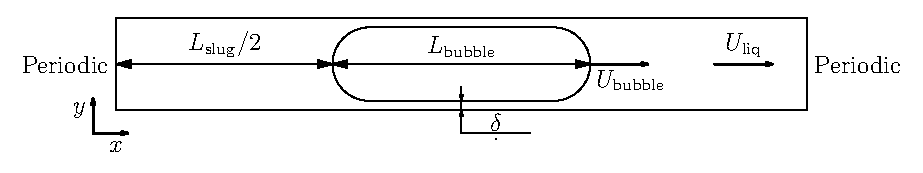
\includegraphics[width=\textwidth]{benchmark_hydro.eps}
\caption{Simplified sketch of the bubble motion. Using periodic
conditions for the velocity field is natural, but needs evaluation for mass
transfer.
\label{fig:benchmark:hydro}}
\end{figure}

To establish numerical procedures we performed multiphase simulations
to extract bubble shapes
\cite{kuzmin-binary2d,kuzmin-binary3d} for the range of capillary numbers
$Ca=0.1\div 1.0$. For this range of capillary numbers
we were able to capture the bubble shape change and the change of hydrodynamic
patterns. The mass transfer simulations presented here were performed with various boundary
conditions (open, periodic) and with a few unit cells ($1$ to $10$ unit cells).
As our numerical approach we take the lattice Boltzmann method, a relatively
new CFD competitor developed during last $20$ years
\cite{frisch,mcnamara,HJ,HSB}. This method was successfully applied to simulate
not only single phase hydrodynamic problems \cite{yu}, but also multiphase
flows \cite{Shan-chen:extended,swift,gunstensen}, heat transfer
\cite{yuan-thermal,zhang-thermal}, and ferrofluids \cite{dellar-ferro,kuzmin-aniso}.

Mass transfer problems in the lattice Boltzmann framework were mainly
addressed in a series of works of Ginzburg and co-authors
\cite{ginzburg-main,ginzburg-boundary-conditions,ginzburg-saturated-flow}.
In contrast to these works whose focus was on simulating the
advection-diffusion equation via the lattice Boltzmann framework, we concentrate
on the application side.  One should also mention the work of \citet{inamuro-scalar-boundary}
about heat and mass transfers in porous media and the work of
\citet{jos-mass} simulating lateral mixing in cross-channel flow.  The last two
works are focused on problems of homogeneous nature and do not provide
guidance as to how to obtain the mass transfer coefficient for heterogeneous cases.

The paper is organized as follows. We start with definitions of the volumetric mass transfer coefficient and apply them 
to the bubble train flow to derive expressions to connect the space- and time-averages.  Then, the lattice
Boltzmann model used to simulate mass transfer is presented, followed by benchmarks. Finally,
numerical simulations of various boundary conditions and simulations spanning a few unit cells for
different hydrodynamic patterns are presented to establish the procedure to determine the
volumetric mass transfer coefficient. The comparison with analytical correlations is also presented.

\section{Mass transfer definitions}
By definition, the mass transfer coefficient from a surface with an imposed constant
concentration $\cbubble$ is:
\beqal
\label{eq:main:definition}
&k_L=\frac{\dot{m}}{P \Delta C},\ \Delta C= \cbubble - \cmedium,
\feqal
where $\dot{m}$ is the mass flux $\Bigl[\frac{kg}{s}\Bigr]$, $P$ is the area of the surface
$\Bigl[m^2\Bigr]$, and $\Delta C$ is the concentration difference between the surface and the surrounding medium
$\Bigl[\frac{kg}{m^3}\Bigr]$. Therefore, $k_L$ has a dimension of 
$\Bigl[\frac{m}{s}\Bigr]$. Usually, the surrounding medium concentration is taken at an infinite distance
from the bubble. However, in the case of complicated geometries and non-homogeneous concentrations, 
the medium concentration can be the average concentration in the domain or the flux-averaged
concentration at the inlet or outlet, etc. Thus, one needs to establish a clear definition of  $\Delta C$ to determine the volumetric
mass transfer coefficient in the case of complex geometries and non-trivial hydrodynamic velocity patterns.

%There exist a number of methods to estimate the mass transfer coefficient $k_L$. 
We first examine the
 definitions of mass transfer in the case of point  sources.
\subsection{Point mass sources}
In what follows we will present three approaches to calculate point  mass transfer
coefficients (by point source we assume the source to have an infinitesimally small surface area $P$):
\begin{enumerate}
\item
Let us look at the infinitesimally small domain of volume $A \Delta x$, not
moving and containing a point source.  The concentration difference is $\Delta C =
\cstar -
C(t)$, where $\cstar$ is the imposed point source concentration, and $C(t)$ is
the time-dependent concentration, which does not depend on the location due to the assumption of
homogeneity. One can therefore write a time-dependent ordinary differential equation for the
concentration in the domain:
\beq
\dot{m}= A \Delta x \frac{\mathrm{d}C}{\mathrm{d} t} = k_L P (\cstar-C(t)), 
\feq
with the initial condition $C(0)=0$.
The solution can be found as:
\beq
C(t)= \cstar (1-\exp(-\vol t )), 
\feq
where $\vol$ is the volumetric mass transfer coefficient defined as:
\beq
\vol=k_L \frac{P}{A \Delta x}=k_L \frac{P}{V},
\feq
where $P$ is the source surface, $V$ is the unit cell volume.
\item
Let us predict mass transfer in a liquid moving with the velocity
$U$, see Fig. \ref{fig:moving:frame}. 
\begin{figure}[htb!]
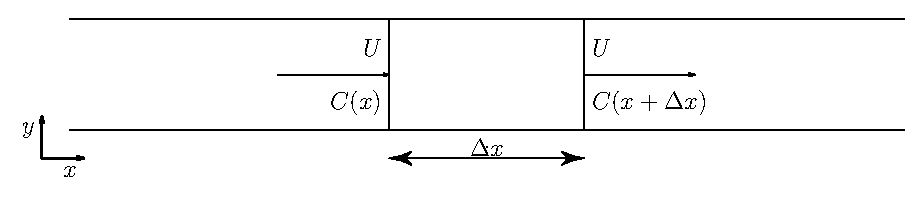
\includegraphics[width=\textwidth]{mass_transfer.eps}
\caption{The mass transfer in a moving liquid. \label{fig:moving:frame}}
\end{figure}

If one can assume that the point mass sources are distributed in the whole
medium, the mass accumulated in the volume $V=A \Delta x$ can be
calculated as the difference of mass fluxes entering and leaving the domain $U
\bigl(C(x+\Delta x)-C(x)\bigr)$. The accumulated mass should be proportional to
the mass transfer coefficient:
\beq
U \bigl(C(x+\Delta x)-C(x)\bigr)=k_L P \bigl(\cstar-C(x)\bigr), 
\feq 
giving the same solution but only in the spatial domain:
\beq
%\label{concentration:domain:coordinate}
C(x)= \cstar \Bigl(1-\exp\bigl(-k_L a \frac{x}{U} \bigr)\Bigr).
\label{main:mass:transfer:expression} 
\feq
Note that the concentration $C(x)$ does not depend on time. 

\item If one transfers to the frame moving with the liquid velocity $U$, the situation will be
the same as in the first case. One can connect  time and space with the
velocity $U$ ($t=\frac{x}{U}$) to obtain the same equation as in the case 2.
\end{enumerate}

\subsection{Bubble train}
In the application to the bubble train flow it is useful to think of one bubble as a point
source to be able to use the calculations presented above. For example, the expression
(\ref{main:mass:transfer:expression}) was used in experiments by
\citet{bercic-mass}. However, one should be accurate with the definition of velocities because two
different phases co-exist in the bubble train flow. Usually, one can take the velocity $U$ to be
a bulk velocity or $U=\ugas+\uliq$, where $\ugas$ and $\uliq$ are liquid and gas
superficial velocities, respectively. 

With experimental measurements of concentration at different locations, the calculation
of the mass transfer coefficient using the logarithmic function is straightforward.
However, if one wants to analytically or numerically calculate the mass transfer coefficients, the
situation is much more complicated because of the presence of two phases and complex bubble
geometry. As was mentioned before, depending on the capillary
number the velocity pattern and thus scalar mixing is different. Analytical approaches
\cite{irandoust,vanbaten-circular} assume that the
contributions from film and bubble caps can be calculated separately. Therefore no tracer from the film influences bubble caps diffusion.   However, this assumption overpredicts mass transfer for a number of experiments \cite{irandoust}. This happens since some tracer
concentration from the film is mixed with the slug and increases the overall concentration in the slug, thereby decreasing
the mass transfer from the bubble caps.
Therefore, the analytical estimates for the mass transfer coefficient calculation  do not account for mutual mass
transfer from neighbouring bubbles.

%Another issue is that if the bubble is long enough then the film saturates with the tracer
%concentration and its influence on mass transfer can be negligible \cite{vanbaten-circular}.
Overall, mixing patterns of the film and liquid slugs are of great importance for the 
estimation of mass transfer \cite{yue-mass}. However, the assumptions usually taken for 
mass transfer calculations are small capillary numbers and certain mixing patterns such as to help to
estimate the mass transfer using the penetration theory of \citet{higbie}.

In comparison with analytical calculations and simplifications, the numerical approach can take into
account the complex mixing patterns and geometries. However, there are challenges as  how to
mimic the continuous picture where the medium is moving with bulk velocity $U=\ugas+\uliq$  as it is done in
experiments. Thus, the questions indicated in Section \ref{intro} arise.  The next section gives more
 details about numerical simulations.
 
\subsection{Numerical simulations}
\label{section:cases}
Ideally one wants to mimic the continuous picture as it is seen in experiments.
Thus, mass transfer simulations for a number of unit cells each containing a bubble are needed. As was
indicated above, there are two approaches towards it -- either to simulate the
bubble train and then to measure concentration along the pipe, Eq.~\ref{main:mass:transfer:expression},
or to transfer to the reference frame moving with the bulk
velocity $U$ and conduct the same measurements. However, both methods require tracking of
moving bubbles which is complicated from the numerical point of view. Therefore, one needs to come
up with a simple and smaller domain for calculations of the mass transfer coefficient, which closely mimics the
continuous picture of a large number of  separated bubbles. 

To avoid complications with moving grids, our
approach is to simulate mass transfer in a reference frame moving with the bubble. Therefore, one
needs to examine  Eq.~\ref{main:mass:transfer:expression} more closely. 

We perform simulations in the frame co-moving with the bubble
in which the bubble position stays constant. The bubble velocity $\ububble$ is
different from the bulk velocity $U=\ugas+\uliq$, and one thus needs to perform a $x$ coordinate
variable change:
\beqal
\label{theor:average:concentration:time}
&x(t)=\ububble t\\
&\overline{C(x)}=\cstar \Bigl(1-\exp\bigl(-\vol \frac{x}{\ugas+\uliq}\bigr)\Bigr)\\
&\langle C(t)\rangle=\cstar \Bigl(1-\exp\bigl(-\vol\, t \frac{\ububble}{\ugas+\uliq}\bigr)\Bigr),
\feqal
where $\langle C(t)\rangle$ is the space-averaged characteristic concentration,
and $\overline{C(x)}$ is the time-averaged concentration at location $x$. 
%The geometry is not one-dimensional and one needs the characteristic concentration
%to be only as a function of time. 
One can make different choices for
$\langle C(t) \rangle$ such as the concentration averaged over the whole domain or inlet/outlet space-averaged
concentrations used in works \cite{vanbaten-circular,kreutzer-overview}.  
%Note that $C(x)$ is not averaged in time as $\overline{C(x)}$ since $C(x)$
%ideally should not depend on time. 
The volumetric mass transfer coefficient can be obtained through the space-averaged concentration:
\beqal
\label{theor:one:concentration:time}
&\vol\, t \frac{\ububble}{\ugas+\uliq}=\ln \frac{\cstar}{\cstar-\langle C(t)\rangle}\\
&\volnondim=\frac{\lunit}{\ububble t}\ln \frac{\cstar}{\cstar-\langle C(t) \rangle},
\feqal
where the parameter $\vol \frac{\lunit}{\ugas+\uliq}$ is non-dimensional. One can also measure the
volumetric mass transfer coefficient from concentrations given at times $t_1$ and $t_2$:
\beq
\label{theor:continuous:mass:transfer}
\volnondim=\frac{\lunit}{\ububble
(t_2-t_1)}\ln\frac{C^{*}-\langle C(t_1) \rangle}{C^{*}-\langle C(t_2) \rangle}.
\feq
Expressions (\ref{theor:average:concentration:time} - \ref{theor:continuous:mass:transfer}) are the
cornerstones of the present work . Four possible scenarios of numerical simulations have been examined: 
\begin{enumerate}
\item % The bubble train multiphase simulations are conducted by applying periodic boundary
%conditions \cite{kuzmin-binary2d,kuzmin-binary3d}. 
%One
%can make an assumption of same boundary
%conditions applied to the tracer concentration to simulate mass transfer. 
One unit
cell is simulated with
periodic boundary conditions, see Fig. \ref{fig:benchmark}. In this case no tracer leaves the
domain similarly to the plug flow. 
%From the physical point of view this case resembles the mass transfer for small Capillary numbers
%$Ca<0.1$.  The liquid slug is well mixed and one have a homogeneous concentration in the unit
%cell, i.e. the outlet and the inlet concentrations are close. 
Though easier to implement, it gives rise to the criticism
that the inlet concentration is equal to the outlet one. As was
discussed, in experiments there is a concentration difference between the
inlet and the outlet, even for one unit cell.

In this case, the volumetric mass transfer coefficient is calculated by Eq. \ref{theor:one:concentration:time}.
The
characteristic concentration $\langle C(t) \rangle$ required for the volumetric mass
transfer coefficient is taken as the average concentration in the domain:
\beq
\label{average:concentration:definition}
C(t)=\frac{\int_{liquid}{C \mathrm{d}V}}{\int{\mathrm{d}V}}.
\feq
\begin{figure}[htb!]
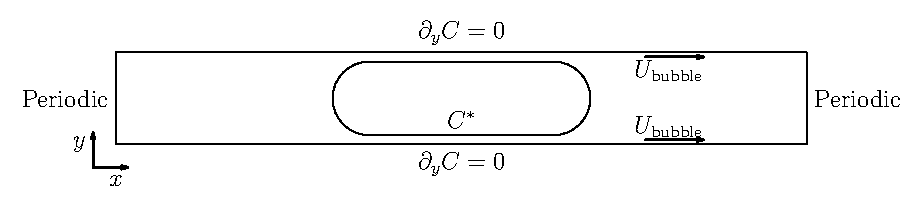
\includegraphics[width=\textwidth]{benchmark_middle.eps}\\
\caption{The two-dimensional benchmarks for the  the mass transfer
coefficient (bottom) for the bubble located near the entrance (top) and at the middle of the domain
(bottom). \label{fig:benchmark}}
\end{figure}
\item Periodic boundary conditions are applied as in the first case but the characteristic concentration is taken as the inlet/outlet flux-averaged
concentration \cite{vanbaten-circular}:
\beqal
&\langle \cinlet(t) \rangle=\frac{\int{U(y) C(0,y,t) \mathrm{d}y}}{\int{U(0,y) \mathrm{d}y}}\\
&\langle \coutlet(t) \rangle=\frac{\int{U(y) C(\lunit,y,t) \mathrm{d}y}}{\int{U(\lunit,y)
\mathrm{d}y}}\\
&\cinlet(\bm{x},t)=\coutlet(\bm{x},t),\,\text{due to periodicity}.
\feqal
The assumptions of this approach are
that the concentration difference between the inlet/outlet- and the space-averaged over the whole unit cell is not significant. Thus, the tracer is assumed to be well mixed in the slug.
\item
The approach of \citet{vanbaten-circular}, where periodic boundary conditions are used and
the mass transfer coefficient is calculated as the gain of the mass in the system
divided by the concentration difference
multiplied by the surface area:
\beq
\label{eq:vanbaten:formulation}
\vol=\frac{\dot{m}}{P \Delta C}\frac{P}{V}=\frac{\dot{m}}{V (\cstar-\langle C(t) \rangle)},
\feq
where the mass flux in the domain can be calculated as:
\beq
\dot{m}=\frac{m_2-m_1}{t_2-t_1}=\frac{\int_{liq}{C(\bm{x},t_2)\mathrm{d}\bm{x}}-\int_{liq}{
C(\bm{x},t_1)\mathrm { d } \bm{x}} } {
t_2-t_1 }.
\feq
In the approach of \citeauthor{vanbaten-circular} the inlet/outlet flux-averaged concentrations were taken as the
characteristic concentration $\langle C(t) \rangle $.

%\item 
%The approach of the opened boundaries was examined, see Fig. \ref{fig:benchmark:jos}. At the inlet
%and outlet boundaries the diffusion flux was imposed to be zero, $\frac{\partial C}{\partial x}=0$.
%The characteristic concentration was taken as the average concentration in the whole domain.
%\begin{figure}
%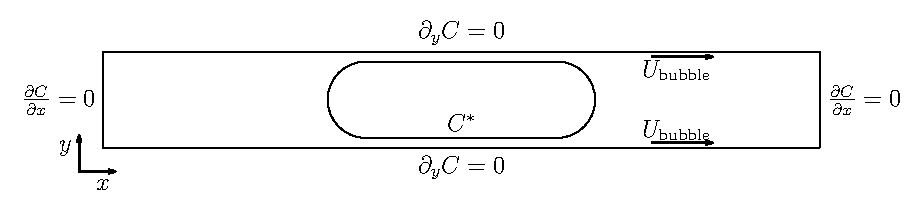
\includegraphics[width=\textwidth]{Figures/benchmark_jos.eps}
%\caption{The numerical mass transfer benchmark with open boundaries. The mass transfer is
%calculated according to Eq. \ref{theor:average:concentration:time} with the characteristic
%concentration accoring to Eq. \ref{average:concentration:definition}. \label{fig:benchmark:jos}}
%\end{figure}
\item 
Simulation of several unit cells, see Fig. \ref{fig:benchmark:alot}. This situation corresponds to the head of the
bubble train, after injection in the pipe and travelling along the channel. One can see that this
situation best resembles the experimental picture, but also requires larger computational
resources. By simulating a certain number of 
bubbles in the train head, the influence of the boundaries can be
reduced. For example, left and right boundary conditions in this case are taken as open boundaries, i.e. $\partial C/ \partial x = 0 $.  There is no ambiguity in the choice of the
characteristic concentration. The average concentration of any unit cell far away from boundaries will be governed
by Eq.
\ref{theor:continuous:mass:transfer}. 
\begin{figure}[htb!]
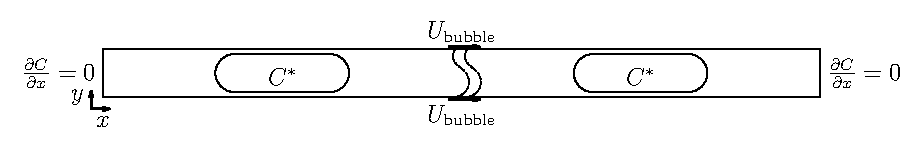
\includegraphics[width=\textwidth]{benchmark_alot.eps}\\
\caption{Benchmark for multiple unit cells. \label{fig:benchmark:alot}}
\end{figure}
\end{enumerate} 

One can notice that all examined cases are the extreme limits of one equation:
\beq
\label{main:main:main}
\vol=\frac{\dot{m}-\int{\coutlet(t) u(\lunit,y)\mathrm{d}y}+\int{\cinlet(t) u(0,y)\mathrm{d}y}}{V
\Delta C}, 
\feq
where $\Delta C=\cstar-\langle C(t) \rangle$ with $\langle C(t) \rangle$ taken to be
the average concentration in the whole liquid domain, $\dot{m}$ is the mass gain in
the domain,$\int{\cinlet u(0,y) \mathrm{d}y}$ and $\int{\coutlet
u(\lunit,y)\mathrm{d}y}$ are inlet/outlet mass fluxes. Eq. \ref{main:main:main}
describes the mass balance: whatever was generated by the bubble surface equals
 the domain mass change minus whatever left the domain plus whatever entered it.

Periodic boundary conditions are the extreme
limiting case of Eq. \ref{main:main:main}: 
\beqstar
\int{\coutlet(t)
u(\lunit,y)\mathrm{d}y}=\int{\cinlet(t) u(0,y)\mathrm{d}y}. 
\feqstar
%Then the mass change in the domain arises only because of the bubble
%surface. However, to calculate the mass transfer coefficient one needs to have
%the characteristic concentration  $\langle C(t) \rangle$ and the mass gain $\dot{m}$
%which do require the storage of both temporal and spatial information.
Another limiting case (will be shown later) is when the mass accumulation rate equals zero, i.e. $\dot{m}=0$. 
This situation corresponds to a simulation of a few unit cells with open boundary for flows with
$Ca>0.7$.   
%One
%can use only spatial information to calculate the mass transfer coefficient,
%i.e. $\int{\cinlet(t) u(0,y) \mathrm{d}y}$ and $\int{\coutlet(t)
%u(\lunit,y)\mathrm{d}y}$ require only space information. 

Before we examine all the test cases above, some lattice Boltzmann mass transfer
benchmarks will be presented. 

\section{Validation}
As was discussed earlier, analytical correlations for the mass transfer coefficient
have been derived for a Taylor bubble train flow  as two separate contributions: the mass transfer from two
half circles and the mass transfer from the film. We will examine these
mass transfer cases closely with the help of the lattice Boltzmann method and compare them
against analytical
solutions. The next sections will give a short introduction to the lattice Boltzmann method and present benchmark results.

\subsection{TRT $D2Q9$ model}
The lattice Boltzmann equation (LBE) operates on a square/cubic grid representing the
physical domain. It utilizes
probability distribution functions (also known as particle populations)
containing information about
macroscopic variables, such as fluid density and momentum. LBE consists of
two parts: a local collision step, and a propagation step which transports
information from one node to another along  
directions specified by a discrete velocity set.
The LBE is typically implemented as follows:
\begin{equation}
\label{standard:implementation}
\begin{aligned}
&f_i^{*}(\bm{x},t)= f_i(\bm{x},t)-\omega \bigl(f_i(\bm{x},t)-eq_i(\bm{x},t)\bigr),&&\text{
collision step}\\
&f_i(\bm{x}+\bm{c_i},t+1)=f_i^{*}(\bm{x},t),&&\text{ propagation step}, 
\end{aligned}
\end{equation}
where $f_i$ is the probability distribution function in the direction $\bm{c_i}$,
 $eq_i$ is the equilibrium probability distribution function, and $\omega$ is the
relaxation parameter. The term $-\omega \bigl(f_i- eq_i\bigr)$ is the so-called BGK
collision operator \cite{bgk}. However, the approach used here is the TRT
(two-relaxation-times) collision operator \cite{ginzburg-main,ginzburg-saturated-flow}. In
comparison with the widely used BGK collision operator, the TRT collision operator has better accuracy
for diffusion and convection fluxes, as well as a larger range of parameters where the scheme is stable.

The TRT collision operator \cite{ginzburg-boundary-main}
decomposes the populations and the equilibrium
distribution into a symmetric and an antisymmetric part:
\begin{equation}
\label{trtdecomp}
f^{\pm}_i=\frac{f_i\pm f_{\bar{i}}}{2}\;,\; 
{eq_i}^{\pm}=\frac{eq_i\pm eq_{\bar{i}}}{2}\;,
\end{equation}
where $\bar{i}$ is the opposite direction to the $i$-th direction.
The collision is performed with two independent relaxation rates for 
symmetric and antisymmetric modes:
\begin{equation}
\label{trt}
\begin{aligned}
&f_i^{*}(\bm{x},t)=f_i(\bm{x},t)-\omegaplus (f_i^{+} - eq_i^+)-\omegaminus
(f_i^{-} -
eq_i^-)\\
&f_i(\bm{x}+\bm{c_i},t+1)=f_i^{*}(\bm{x},t).
\end{aligned}
\end{equation}
Note that the TRT collision operator reduces to the BGK operator if
$\omegaplus=\omegaminus$. In comparison with the BGK collision operator,
the TRT collision operator has one additional degree of freedom. The TRT operator 
introduces
the following free parameter
$\Lambda=\Bigl(\frac{1}{\omegaplus}-\frac{1}{2}\Bigr)\Bigl(\frac{1}{\omegaminus}-\frac{1}{2}
\Bigr)$. 
This free parameter controls the effective location of  bounce-back
walls \cite{ginzburg-multireflection}, second-order accuracy of
boundary \cite{ginzburg-boundary-main} and interface schemes \cite{ginzburg-discontinious}, 
spatial accuracy \cite{ginzburg-recurrence,servan-trt-stability},
consistency \cite{ginzburg-brinkman} and, to some extent,
stability \cite{kuzmin-stability-optimal,kuzmin-d1q3,servan-trt-stability}.
In particular, $\Lambda=\frac{1}{4}$ achieves the optimal stability for the
isotropic advection-diffusion equation \cite{kuzmin-stability-optimal}. 

The parameters $\omegaplus$, $\omegaminus$ and $eq_i$ fully define the lattice Boltzmann
procedure. The two-dimensional, nine-velocity LBM $D2Q9$ we used in this work is defined on the set
of lattice
velocities with components:
\beqal
&c_{ix}=\{0,1,0,-1,0,1,-1,-1,1\},\text{ for } i=0\dots8\\
&c_{iy}=\{0,0,1,0,-1,1,1,-1,-1\},\text{ for } i=0\dots8\,.
\feqal

The equilibrium functions for the $D2Q9$ TRT model are represented as \cite{kuzmin-stability-optimal}:
\begin{equation}
\begin{aligned}
&eq_i^{+}=eq_i^{(m)}+g^{(u)} eq_i^{(u)}\\
&eq_i^{(m)}=t_i^{(m)} c_e+ eq_i^{(a)}\\
&eq_i^{(u)}=t_i^{(u)} \frac{u_x^2+u_y^2}{2}+\frac{u_x^2-u_y^2}{4} p_i^{(xx)}+g_{xy}^{(u)}\frac{u_x
u_y}{4} p_i^{xy}\\
&eq_i^{(a)}=\frac{K_{xx}-K_{yy}}{4} p_i^{xx}+\frac{K_{xy}}{4} p_i^{(xy)}\\
&eq_i^{-}=t_i^{(a)}  u_{\alpha} c_{i\alpha},
\end{aligned}
\end{equation}
where $K_{xx,yy,xy}$ are proportional to components of the diffusion tensor,
$c_e=\frac{K_{xx}+K_{yy}}{2}$, parameters $g^{(u)}$ and $g^{u}_{xy}$ are either zero or one (see
below), the tensor $p_i^{(xx)}=c_{ix}^2-c_{iy}^2$, the tensor $p_i^{(xy)}=c_{ix} c_{iy}$, the
weights
$t_i^{(u,m,a)}$ can be chosen based on stability criteria. The most commonly used set of weights, the so-called
``hydrodynamic`` weights, were chosen:
\begin{equation}
t_i^{(u)}=t_i^{(m)}=t_i^{(a)}=\Bigl\{0,\frac{1}{3},\frac{1}{3},\frac{1}{3},\frac{1}{3},\frac{1}{12},
\frac {1}{12},\frac{1}{12},\frac{1}{12}\Bigr\}
\end{equation}
 
It can be shown through the Chapman-Enskog procedure \cite{chapman}, that the simple update rule
with the equilibrium function presented above restores the anisotropic
advection-diffusion equation:
\beq
\partial_t C+ \partial_{\alpha} C u_{\alpha}=\partial_{\alpha\beta} D_{\alpha\beta} C,
\feq
where the concentration $C=\sum_i{f_i}$, and $D_{\alpha\beta}=\Bigl(\frac{1}{\omegaminus}-\frac{1}{2}\Bigr)K_{\alpha\beta}$ is the
following diffusion tensor:
\begin{equation}
D_{\alpha\beta}=
\begin{pmatrix}
D_{xx} + \Bigl(\frac{1}{\omegaminus}-\frac{1}{2}\Bigr)(g^{(u)}-1) u_x^2 &
D_{xy}+\Bigl(\frac{1}{\omegaminus}-\frac{1}{2}\Bigr)(g_{xy}^{(u)}-1)u_x u_y\\
D_{xy} + \Bigl(\frac{1}{\omegaminus}-\frac{1}{2}\Bigr)(g_{xy}^{(u)}-1) u_x u_y&
D_{yy}+\Bigl(\frac{1}{\omegaminus}-\frac{1}{2}\Bigr)(g^{(u)}-1) u_y^2. 
\end{pmatrix}
\end{equation}
We want to resolve the isotropic advection-diffusion equation, $D=D_{xx}=D_{yy}$ or
$K=K_{xx}=K_{yy}$, with the non-diagonal diffusion tensor components set to zero ($D_{xy}=0$). In
contrast to the $D2Q5$ model, with $D2Q9$ it is
possible to cancel the numerical diffusion by the proper choice
of the equilibrium functions, i.e. $g_{xy}^{(u)}=g^{(u)}=1$.  The particular choice of parameters
used in simulations is $c_e=\frac{1}{3}$, $\Lambda=\frac{1}{4}$. Thus, the diffusion coefficient $D$
is matched through $\omegaminus$, i.e. $D=c_e
\Bigl(\frac{1}{\omegaminus}-\frac{1}{2}\Bigr)=\frac{1}{3}(\frac{1}{\omegaminus}-\frac{1}{2}\Bigr)$.
For the particular choice $\Lambda=\frac{1}{4}$, $\omegaplus$ can be found easily as
 $\omegaplus=2-\omegaminus$.  

%Fig. \ref{stability:d2q9} shows the stability limits for the $D2Q9$
% model $c_e$ against $U^2=u_x^2+u_y^2$ for two particular choices.
% \begin{figure}[htb!]
% 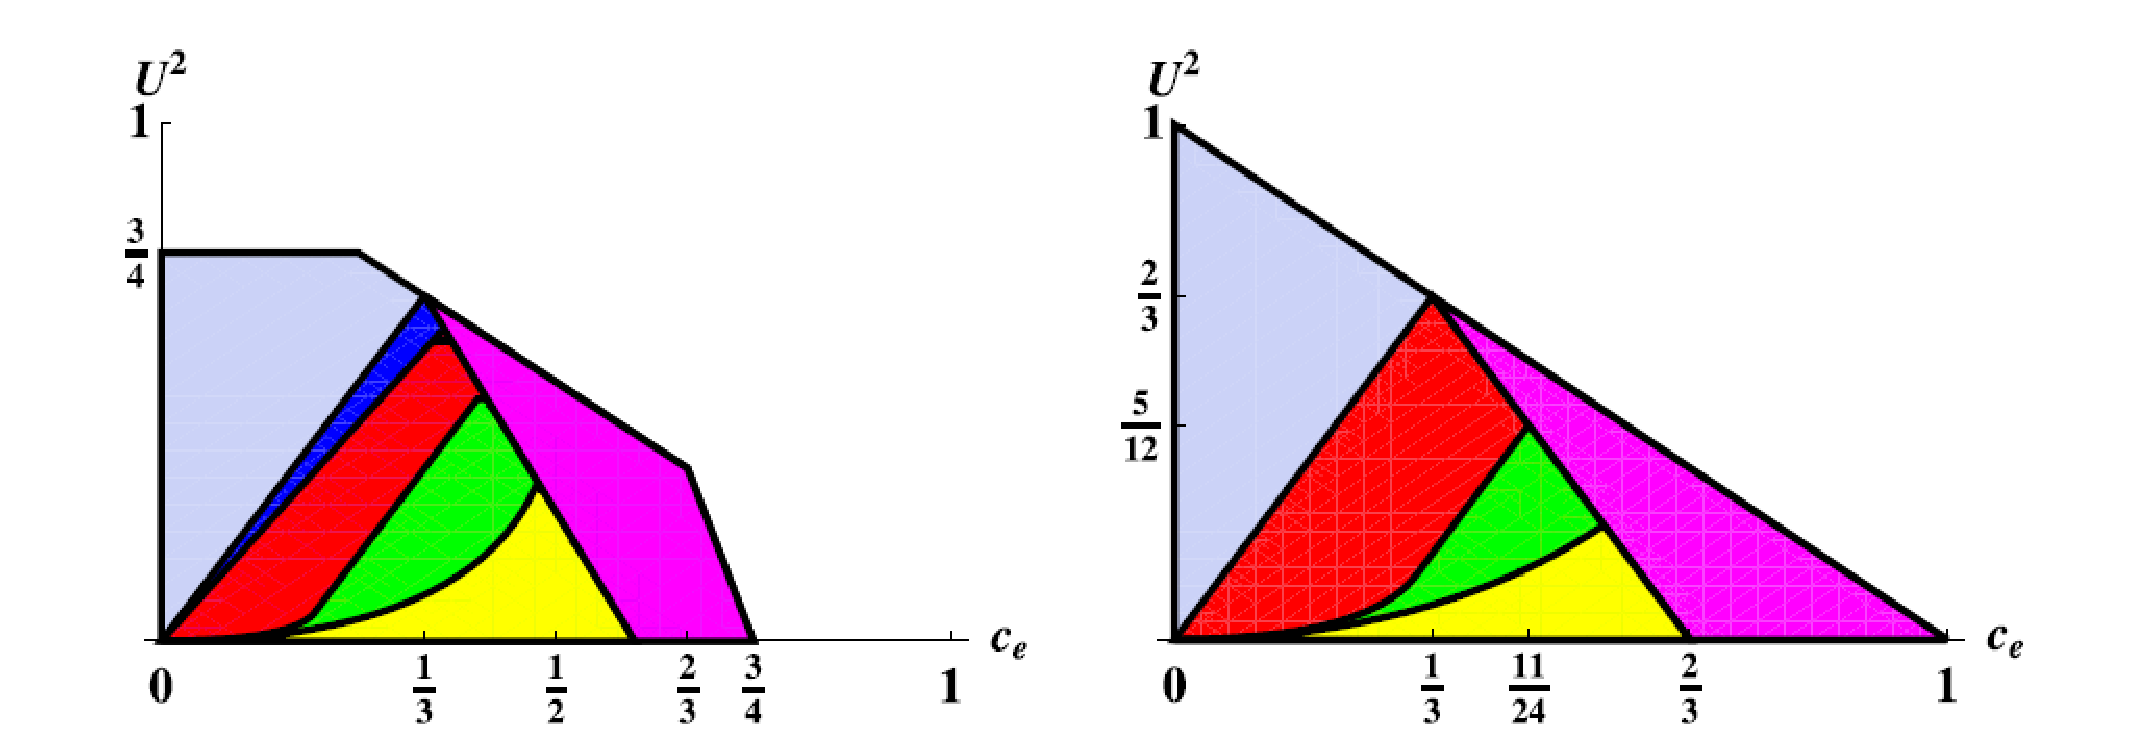
\includegraphics[width=\textwidth]{Figures/d2q9_stability.eps}
% \caption{The stable sub-domains of the $D2Q9$ schemes ($\Lambda=\frac{1}{4}$)
% are plotted for standard (hydrodynamic) weights (left) and uniform weights (right, not mentioned
%here) when the
% numerical diffusion is removed, partially or completely. For particular choice used in this work
%(hydrodynamic weights, $c_e=\frac{1}{3}$, left picture), the achieved stable velocity is
%$u_x^2+u_y^2\leq\frac{2}{3}$. The non-negativity of populations (green+yellow) is for BGK
%stability. One can see that the achieved maximum stable velocity is twice smaller $u_x^2+u_y^2\leq
%\frac{1}{3}$ for the BGK collision operator.The proper choice of weights can
% allow to obtain  total triangle $0 \leq u_x^2+u_y^2 \leq 1- c_e$ (the
% uniform weights only).
% \label{stability:d2q9}}
% \end{figure}

%Boundary conditions for the mass transfer used in this work are all of Dirichlet type. 
We validated
two types of boundary conditions: Inamuro boundary conditions \cite{inamuro-scalar-boundary} and
pressure anti bounce-back boundary conditions \cite{ginzburg-multireflection}. However, the
simulation results  are presented only for pressure anti bounce-back due to their ability
to handle complex boundaries in a simple way:
\beq
\label{antibb}
f^{*}_{B,i}=-f^{*}_{F,\bar{i}} + 2 eq^+(\cstar,\bm{u}),
\feq
where $\cstar$ is the concentration to be imposed at the surface, $\bm{u}$ is the surface velocity,
$i$ is the direction number pointing to the domain located at the boundary surface $B$,
$\bar{i}$ is the direction number opposite to $i$ and is located at the fluid node $F$ specifically
so that node $B$ is located at the location $F+\bm{c_i}$. 

Note that the parameters of the lattice
Boltzmann scheme are connected with  physical parameters only through  non-dimensional
numbers governing the physics of the problem. In our case, this number is the Peclet number, $Pe=\frac{\ububble L}{D}$.
Therefore, one can choose any quantity, for example 
$\ububble$ in the lattice Boltzmann units as long as the
Peclet number is  matched in physical space and numerical simulations. The fact that $\ububble$
can be varied in certain ranges  is extremely useful in the context of numerical simulations. This allows to 
increase the time step and decrease the computational demand (by an order of magnitude). 
% while still obtaining meaningful results. 
This point will be used in simulations and covered later. 

% TODO: I'm not sure I understand this sentence.  Does it say that we use the cap + film simplification
% for the simulations, or that the simulation results are compared to results obtained via this simplification?
The next section will cover LBM benchmarks that resemble the mass transfer from a bubble 
(mass transfer to the liquid with the parabolic velocity profile  and mass transfer from a cylinder).

\subsection{The radial case}
The case to be examined  is the mass transfer from a circle with radius $a$, with the circle approximated as a stair-case. It
can be described by the following system of equations:
\beq
\begin{aligned}
&\partial_t C(r,t)=\frac{1}{r}\partial_r r \partial_r C(r,t)\\
&C(a,t)=C_0,\,C(r,0)=C_{init}
\end{aligned}
\feq 
The analytical solution is \cite{chemical-correlations}:
\beq
\frac{C(r,t)-C_{0}}{C_{init}-C_{0}}=\sum_{n=1}^{\infty}{\frac{2}{\mu_n
J_1(\mu_n)}\exp\Bigl(-\mu_n^2 \frac{D t}{a^2} \Bigr)J_0\left(\mu_n \frac{r}{a}\right)},
\feq
where $\mu_n$ is the $n$-th zero root of the $0$th order Bessel polynomial $J_0(\mu_n)=0$. Some of
the corresponding roots are as follows: $\mu_1=2.4048$, $\mu_2=5.5201$, $\mu_3=8.6537$,
$\mu_4=11.7915$, $\mu_5=14.9309$.
By taking the initial concentration as $0$, one obtains:
\beq
\label{eq:analytical:profile:radial:case}
C(r,t)=C_0 \Biggl(1 - \sum_{n=1}^{\infty}{\frac{2}{\mu_n
J_1(\mu_n)}\exp\Bigl(-\mu_n^2 \frac{D t}{a^2} \Bigr)J_0(\mu_n \frac{r}{a})}\Biggr).
\feq

The solution depends only on the non-dimensional time: $\tau=\frac{D t}{a^2}$. The domain size was $129\times 129$ with the circle radius $a=40$  lattice units. Some results for
different diffusion coefficients are presented in Fig.\ref{fig:cylinder:benchmark}. The numerical simulations with the bounce-back boundary conditions are able to accurately reproduce the analytical results.
\begin{figure}[htb!]
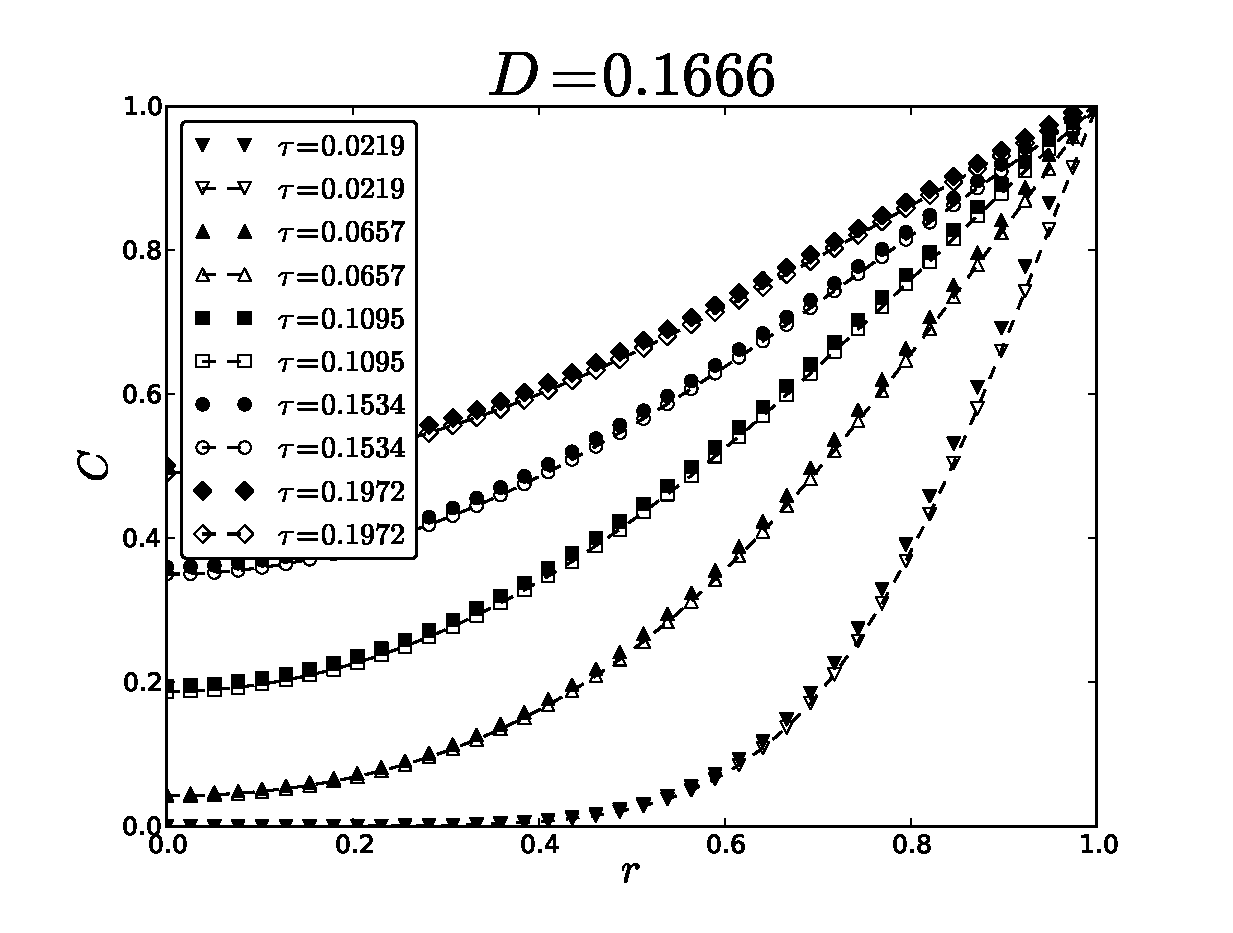
\includegraphics[width=0.5\textwidth]{cylinder1666.eps}
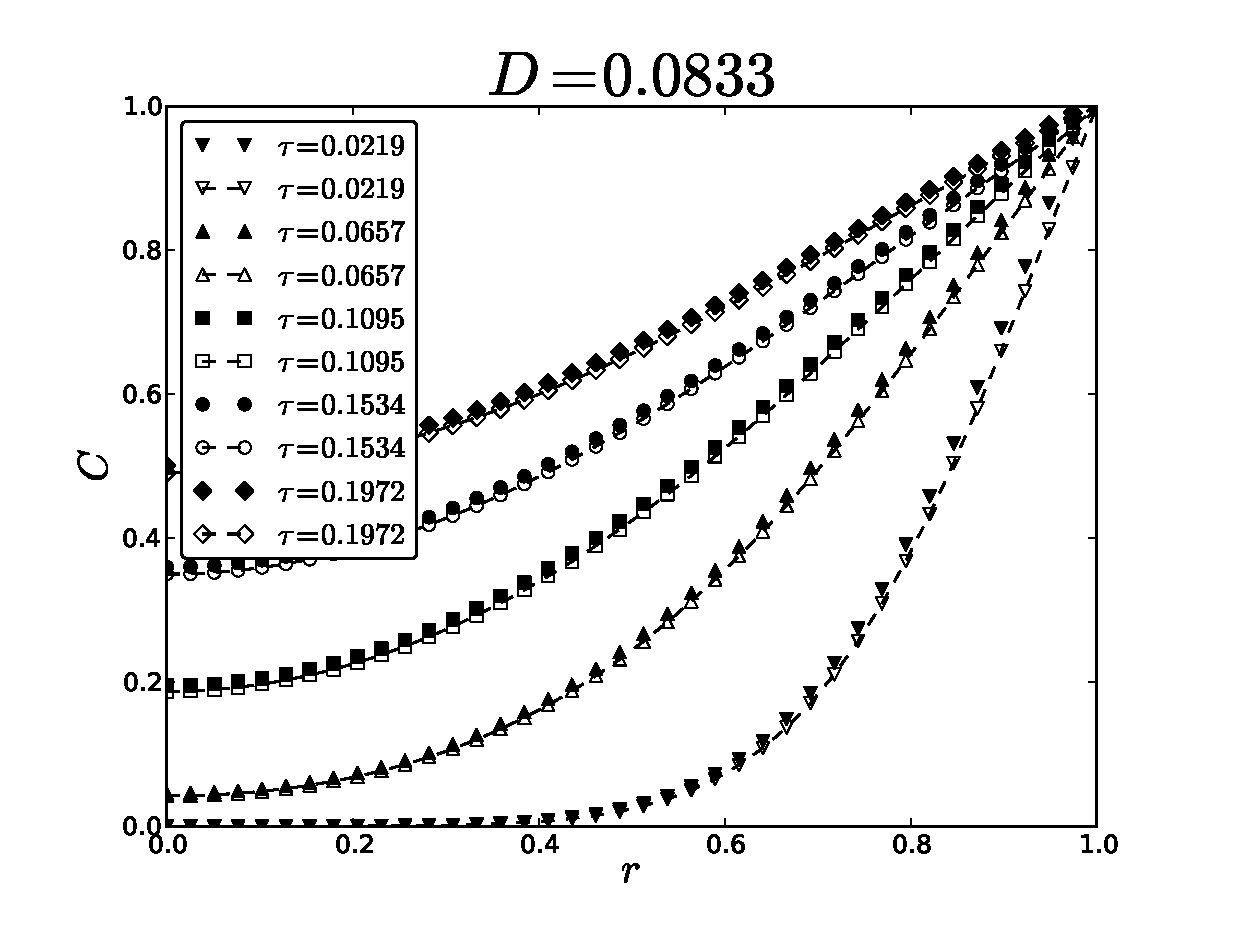
\includegraphics[width=0.5\textwidth]{cylinder0833.eps}\\
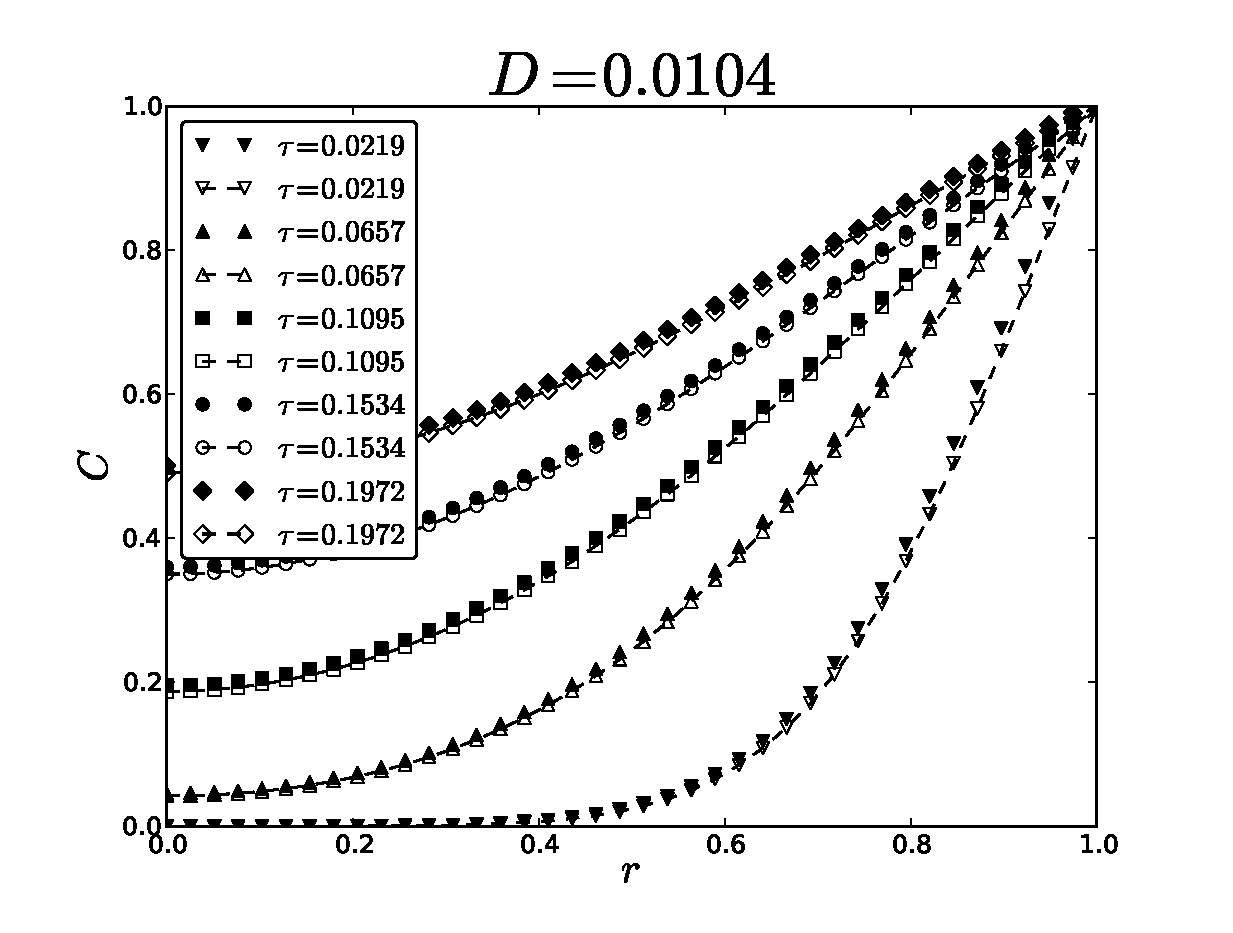
\includegraphics[width=0.5\textwidth]{cylinder0104.eps}
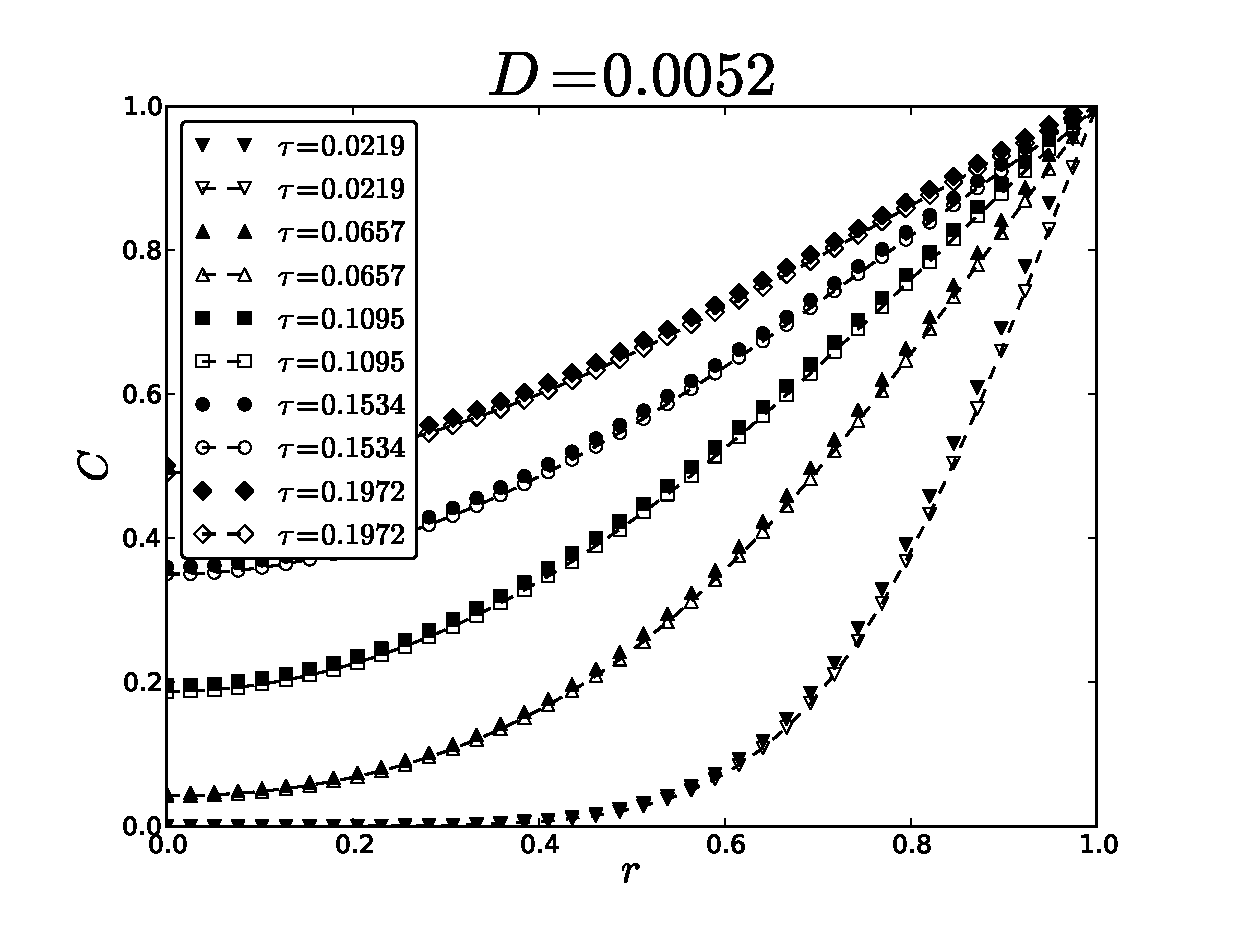
\includegraphics[width=0.5\textwidth]{cylinder0052.eps}\\
\caption{Profiles for different diffusion parameters varied with $\omegaminus$ (lines: Eq. \ref{eq:analytical:profile:radial:case}, symbols: LB results). One can see that the
diffusion from curved boundaries is captured
accurately \label{fig:cylinder:benchmark}. $r$ is the distance from the center. %The profiles are taken along  the axis $x$.
}
\end{figure}

%\subsection{Parabolic velocity profile with the  zero velocity gradient at the wall}
%The problem is defined in terms of the PDE as follows: 
%\beq
%\begin{aligned}
%&\frac{\partial C}{\partial x} U(y)=D\frac{\partial^2 C}{\partial y^2}\\
%&C(0,y)=C_0,\, C(x,0)=\cstar,\, \frac{\partial C}{\partial y }(x,\delta)=0\\
%&U(y)=U_0 \Bigl(\frac{y}{\delta}\Bigr)^2.
%\end{aligned}
%\feq
%The procedure to solve this PDE analytically is presented in Appendix \ref{appendix:zero:gradient}. The result is:
%\beq
%\label{analytical:solution:zero:gradient}
%\begin{aligned}
%&C(x,y)=\cstar+\sum_{m}{C_m
%\sqrt{\frac{y}{\delta}}J_{\frac{1}{4}}\Bigl(\frac{m^2}{2}\frac{y^2}{\delta^2}\Bigr)\exp\Bigl(-\frac{
%m^4 } { Pe }
%\frac { x }{\delta}\Bigr)}\\
%&C_m = (C_0-\cstar) \frac{\int_{\xi=0}^{1}{\xi^{5/2} J_{\frac{1}{4}}\Bigl(\frac{m^2
%\xi^2}{2}\Bigr)\mathrm{d}\xi}}{\int_{\xi=0}^{1}{\xi^3 J_{\frac{1}{4}}^2\Bigl(\frac{m^2
%\xi^2}{2}\Bigr)\mathrm{d}\xi}}
%\end{aligned}
%\feq
%Fig. \ref{fig:parabolic:zero:gradient} shows a comparison contours between the
%analytical solution and the simulation with anti bounce-back boundary conditions used to impose constant
%concentrations at the wall $\cstar=1$ and the inlet $C_0=0$. The simulation grid is
%$80\times1600$. Parameter $\omegaminus=1.8$ implies the diffusion coefficient to be
%$D=\frac{1}{3}\Bigl(\frac{1}{\omega}-\frac{1}{2}\Bigr)=0.0185$.  
%\begin{figure}[htb!]
%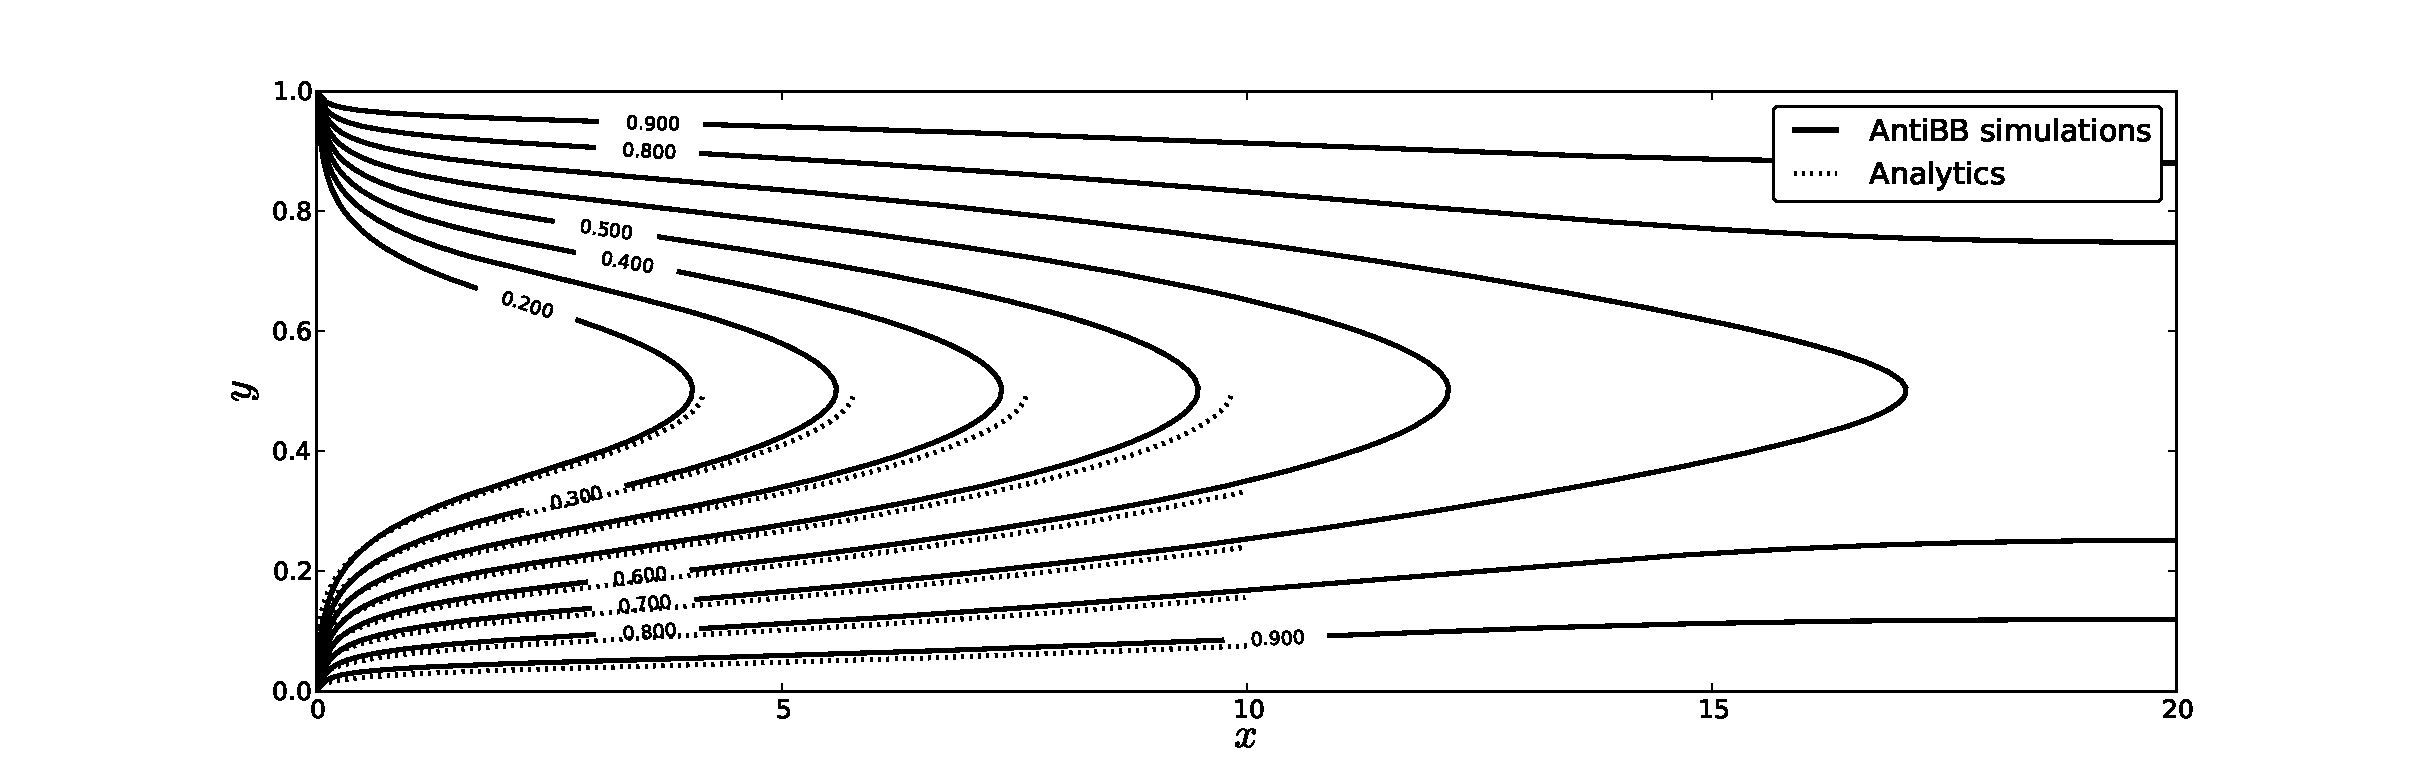
\includegraphics[width=\textwidth]{Figures/parabolic_profile_zero_gradient_comparison.eps}
%\caption{Comparison of the concentration contour levels between the analytical solution, Eq.
%\ref{analytical:solution:zero:gradient}, and simulation for the diffusion coefficient $D=0.0185$. $\delta=H/2$ is half of the channel height (symmetry is used for the sake of simplicity) . The simulation was
%performed on the grid size of $80\times 1600$. The constant concentration is imposed with the
%anti bounce-back conditions, Eq. \ref{antibb}. Coordinate $x$ and $y$ are non-dimensionalized on
%the height of the channel. 
%\label{fig:parabolic:zero:gradient}}
%\end{figure}
 
\subsection{Poiseulle velocity profile}
The problem we want to address can be formulated through the following PDE:
\beq
\begin{aligned}
&\frac{\partial C}{\partial x} U(y)=D\frac{\partial^2 C}{\partial y^2}\\
&C(0,y)=0,\, C(x,\pm \delta)=\cstar,\, \frac{\partial C}{\partial y }(x,0)=0\\
&U(y)=U_0 \Bigl(1-\bigl(\frac{y}{\delta}\bigr)^2\Bigr)
\end{aligned}
\feq
The procedure to solve this problem is presented in Appendix \ref{appendix:poiseuille} which yields
the final solution as:
\begin{equation}
C=\cstar-\cstar \sum_{m=0}{C_m e^{-m^4 \frac{x}{\delta}\frac{1}{Pe}} e^{-m^2
y^2/(2\delta^2)}{_1F_1}\Bigl(-\frac{m^2}{4}+\frac{1}{4},\frac{1}{2},m^2 \frac{y^2}{\delta^2}\Bigr)},
\end{equation}
where coefficients $C_m$ are taken from Eq. \ref{coeff:series:parabolic:profile}. The comparison
between contours of analytical and simulation results is presented in Fig.
\ref{fig:parabolic:comparison}. Parameters were taken as: $D=0.0185$, the grid dimension is $80\times1600$. The centerline velocity is  $U_0=0.05$
which yields the Peclet number $Pe=U_0 \delta / D= 108.108$.
The results are in good agreement. The simulations capture accurately the singular derivative for $x=0$.
\begin{figure}[htb!]
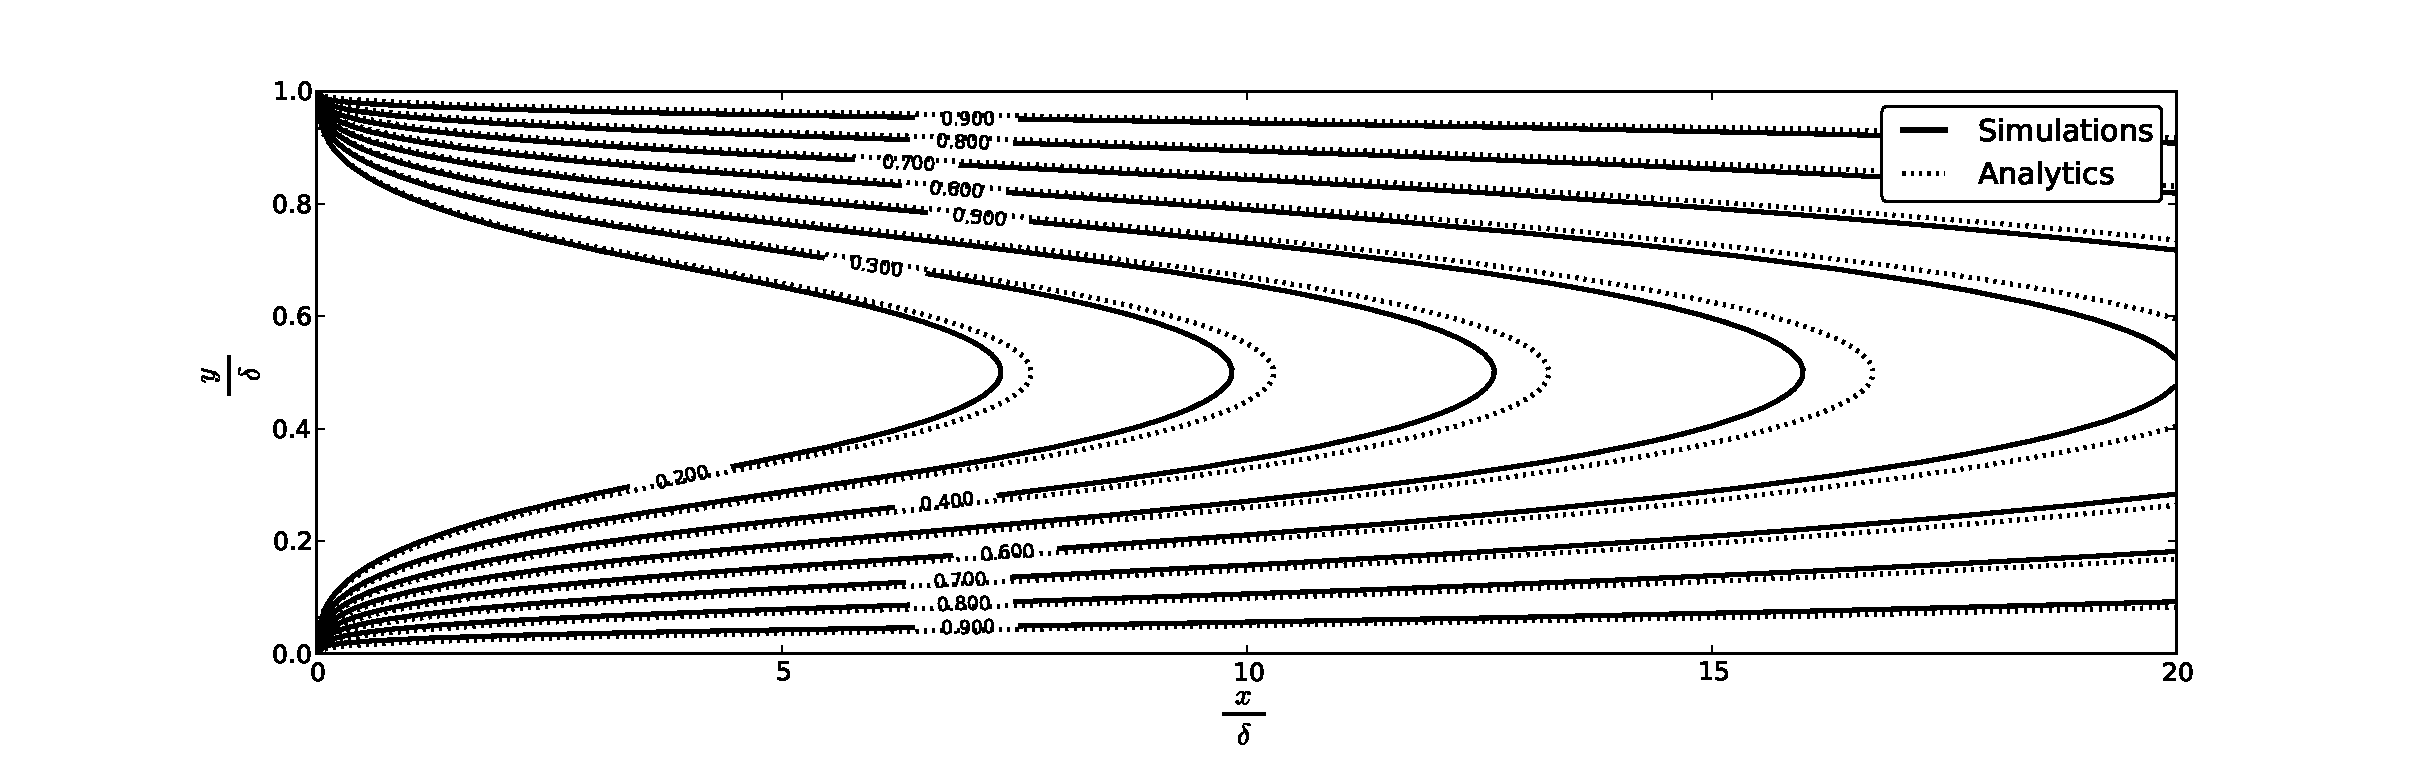
\includegraphics[width=\textwidth]{parabolic_profile_comparison.eps}
\caption{Comparison between the analytical concentration contours and simulations with pressure
anti bounce-back conditions, Eq. \ref{antibb}. The simulation was done for $D=0.0185$ with a
$80\times1600$ grid. The centerline velocity is $U_0=0.05$, and the Peclet number is $108.108$. \label{fig:parabolic:comparison}}
\end{figure}

Now the LBM is validated against the benchmarks relevant for the flow around bubbles, one can
examine the cases mentioned in Section
\ref{section:cases} to calculate the volumetric mass transfer coefficient for Taylor bubble train flow.

\section{Numerical approach}
\label{sec:numerics}
A multiphase code was utilized to obtain the flow patterns and bubble shapes for different capillary numbers
\cite{kuzmin-binary2d}. Five particular cases were chosen to be examined, their results are summarized
in Table \ref{table:capillary:cases}. 
\begin{table}[htb!]
\begin{tabularx}{\textwidth}{|X|X|X|X|X|X|X|X|X|}
\hline
$Ca$    &$Re$     &$\ububble$ &$\delta$&$\holdup$
&$\uliq$&$\ugas$&$\lbubble$&$\lslug$\\
\hline
$0.097$ &$1.656$  &$0.0055$ &$0.092$ &$0.30$ &$0.0046$&$0.0016$&$5.79$&$9.21$\\ 
$0.254$ &$4.318$  &$0.0143$ &$0.132$ &$0.28$ &$0.0108$&$0.0041$&$6.12$&$8.88$\\ 
$0.526$ &$8.938$  &$0.0297$ &$0.157$ &$0.27$ &$0.0209$&$0.0080$&$6.19$&$8.81$\\
$0.750$ &$12.744$ &$0.0424$ &$0.167$ &$0.25$ &$0.0293$&$0.0107$&$5.96$&$9.04$\\
$1.040$ &$17.665$ &$0.0588$ &$0.177$ &$0.22$ &$0.0397$&$0.0135$&$5.59$&$9.41$\\
\hline
\end{tabularx}
\caption{Sample results with the binary liquid lattice Boltzmann model \cite{kuzmin-binary2d}. The
following notations are used: the capillary number $Ca=\frac{\ububble L}{\rho \nu_{\mathrm{liq}}}$, $\uliq$ is the superficial liquid velocity, $\ugas$ is the
superficial gas velocity. $\delta$ is the
non-dimensional film thickness, $\lbubble$ and $\lslug$ are the non-dimensional bubble and slug lengths (defined in channel heights).The simulation sketch is presented in Fig.
\ref{fig:benchmark:hydro}. \label{table:capillary:cases}}
\end{table}
Note that the velocities (LB system) in Table \ref{table:capillary:cases} are small. This means that to
match large Peclet numbers, $Pe=\frac{\ububble L}{D}$, usually used in experiments, one needs to decrease the diffusion coefficient
$D=\frac{1}{3}\Bigl(\frac{1}{\omegaminus}-\frac{1}{2}\Bigr)$. Thus, the parameter $\omegaminus\approx 0.5$. However, for such values of 
$\omegaminus$ the stability of the lattice Boltzmann method drastically decreases
\cite{kuzmin-d1q3}. On the other hand, one iteration in the lattice Boltzmann system corresponds
to a physical time step  $\Delta t=U_{\mathrm{bubble,LB}} \frac{\Delta
x}{U_{\mathrm{bubble,phys}}}$. The iteration time is proportional to the velocity $U_{\mathrm{LB}}$
and the typical number of simulation steps to obtain the steady-state mass transfer coefficient for
$Ca<0.2$ is of the order of a few million. Therefore, it is desirable to increase    $U_{\mathrm{LB}}$
while maintaining the Peclet number. If one increases the velocity, then
$\omegaminus$ increases as well, which impacts positively on the stability of the LBM.
 
Given all the considerations above, mass transfer simulations are performed as follows:
\begin{description}
 \item[Flow field] Given a capillary number $Ca$, one needs to obtain hydrodynamic fields around
the bubble using the multiphase binary liquid lattice Boltzmann model according to our previous work
\cite{kuzmin-binary2d}. Periodic boundary conditions were used in that work. The grid used  was
$202\times 3000$ which corresponds to the fluid domain  of size $200\times3000$. That grid resolution was
taken to ensure grid
independency of the results \cite{kuzmin-binary2d}. Note that we do not approximate bubble shapes by correlations, but we directly resolve them by using the multiphase solver. 
 \item[Bubble reference frame] Once the hydrodynamics is solved, the mass transfer simulations
are conducted in the reference frame moving with the bubble, where the bubble stands still and the liquid
flows around the
bubble. We impose a uniform and steady concentration on the surface
of the bubble with the anti bounce-back condition, Eq. \ref{antibb}.
 \item[Velocity improvement] One can scale the velocity to
perform faster simulations. However, before doing it one needs to improve the velocity field.
This issue arises because of the
multiphase model used in the flow simulations. The binary liquid lattice Boltzmann model is a diffuse
interface model where no clear boundary between gas and liquid exists.
% TODO: Is this only a problem of how we determine the bubble shape or also a problem of
% spurious velocities within the model itself?
We obtain the bubble shape by imposing a condition on the order parameter field $\phi$ with $\phi\leq0$ in the bubble \cite{kuzmin-binary2d}. The velocity of the
bubble is defined as the bubble tip velocity. Because of the square grid, the shape of the bubble is determined within an accuracy of one grid spacing. Thus,
there is an error in the determination of the bubble velocity. Though these errors are small,
there is still a small non-zero velocity component pointing into the bubble in some places, see Fig. 8 in
\cite{kuzmin-binary2d} where some streamlines are penetrating the bubble surface.
This small velocity is amplified upon the velocity scaling and is inconsistent with the
advection-diffusion equation leading to instability after many iterations.

Thus, before performing the mass transfer simulations an additional single phase hydrodynamic
simulation is performed. A free-surface solver was developed in order to obtain a velocity field
consistent with the advection-diffusion equation. We take results from the
multiphase simulations, extract a
bubble shape using the phase indicator $\phi\leq0$, and approximate the bubble shape by the stair-case
line with imposed free-slip boundary condition on it. The obtained bubble velocity is then imposed on the walls. This corresponds to conducting 
simulations in the reference frame moving with the bubble. Appendix \ref{appendix-free-surface} covers the simple
free-slip boundary condition implementation drastically improving velocity patterns. The system is
iterated until a
steady state is reached. Note, that these type of simulations are much faster than the original
multiphase simulations. As the output all the non-zero velocity components perpendicular to the
bubble surface are completely eliminated. We compared original multiphase simulations with
one-component free-slip simulations. All quantities such as superficial slug and liquid velocities are
within $3\%$ for the capillary number in the range $0.05\leq Ca \leq 1.0$. 
One can see in Fig. \ref{fig:streamlines:tweaked:velocity} two streamline profiles for $Ca=0.097$  and $Ca=1.040$.
\begin{figure}[htb!]
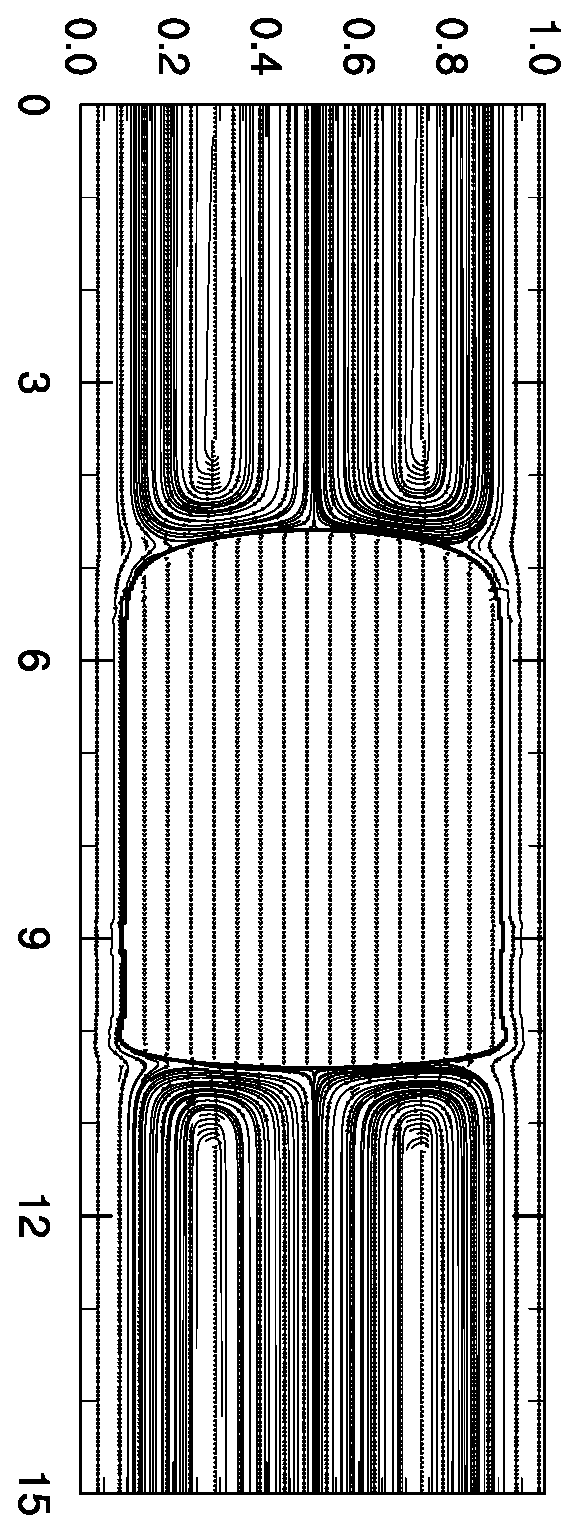
\includegraphics[angle=90,width=\textwidth]{performed_ca0097_out.eps}\\
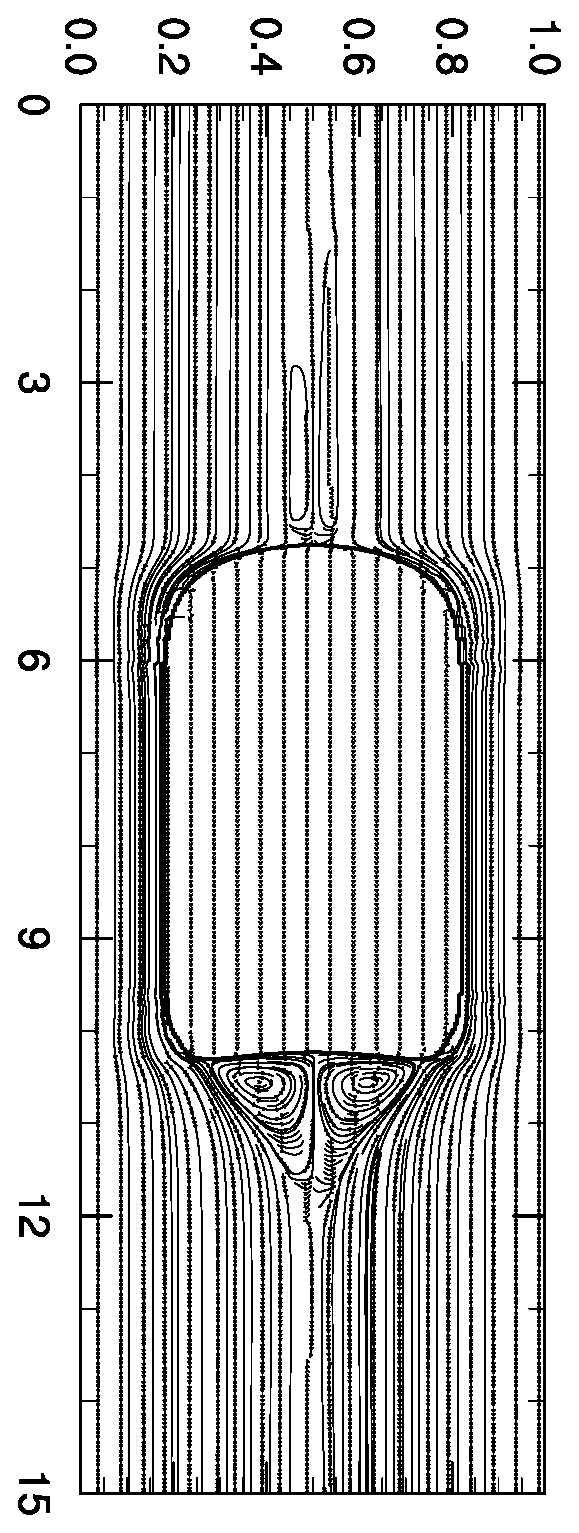
\includegraphics[angle=90,width=\textwidth]{performed_ca1040_out.eps}
\caption{The streamline patterns produced by the free-surface flow solver with simplified approximation
of the free-slip bubble surface, see Appendix \ref{appendix-free-surface}. Two completely different
velocity patterns are obtained, $Ca=0.097$ (top) and $Ca=1.040$ (bottom).
\label{fig:streamlines:tweaked:velocity}}
\end{figure}

\item[Mass transfer] After improved velocity profiles are obtained one can perform any mass
transfer simulations with the various boundary conditions as covered in Section \ref{section:cases}.
For this purpose one needs to match the Peclet number $Pe$ taken from experiments. 
%Note that we
%specifically separated the hydrodynamic problem from the mass transfer problem. 
\end{description}
%When one wants to
%solve these simultaneous problems, then one needs to match all the non-dimensional parameters, as
%the capillary number (viscous forces over surface tension), the Schmidt number (viscous diffusion
%rate over mass diffusion rate), the Peclet number (convection over diffusion), the Reynolds number
%(inertia over viscous forces). As the output one can obtain the Sherwood number  (convection mass transfer over diffusion mass transfer) dependancy on other
%parameters:
%\begin{equation}
%\begin{aligned}
%&Re=\frac{\ububble L}{\nu_{\mathrm{liq}}},&&Ca=\frac{\ububble \mu_{\mathrm{liq}}}{\gamma}\\
%&Pe=\frac{\ububble L}{D},&&Sh=\frac{K L}{D}\\
%&Sc=\frac{\nu_{\mathrm{liq}}}{D}.&&
%\end{aligned}
%\end{equation}
%\end{description}
%Note that in this work we do not establish the Sherwood number dependancy on other parameters in this work. The purpose of this work is to establish procedures of simulation mass transfer problems for the Bretherton/Taylor bubble flow in the context of the lattice Boltzmann simulations.

\section{Results}
This section covers simulation results. We first examine the possibility to increase the fluid
velocity while keeping the Peclet number the same. After that  the results for  periodic boundary
conditions for $5$ capillary number cases will be presented. Finally, we will examine
many
cell simulations for two representative velocity patterns related to $Ca=0.0907$ and $Ca=1.04$ respectively 
(see Fig. \ref{fig:streamlines:tweaked:velocity}). 

\subsection{Velocity scaling at constant Peclet number}
\label{section:keeping:peclet}
This section addresses the process of significantly increasing the
velocity magnitude while keeping dimensionless parameters the same to
speed up                                      
simulations. This is especially important to be able to simulate a few unit cells in a reasonable time.
For example, ten unit cell simulations require a grid of $30000\times202$ nodes.
%Increasing velocity can also help to resolve a lot of unit cells to represent a
%continous picture.
Since the Peclet number is the only dimensionless quantity governing
the advection-diffusion equation:
\beq
Pe=\frac{\ububble N_y}{D}.
\feq
one needs to increase the diffusion coefficient when the velocity is increased. Simulation runs were made with
velocities $2,4,6,8,10,15,20,40$ times larger than the original velocities. The velocities and
their corresponding capillary numbers are presented in Table \ref{table:scaling:peclet}. Periodic
boundary conditions were used and the mass transfer coefficient was calculated according to Eq.
\ref{main:simulation:equation}. Table \ref{table:scaling:peclet} shows that the velocity limit
for  periodic boundary conditions is $0.1$, so to be on the safe side, velocities should not be scaled
up beyond that value.  For example, in Table \ref{table:scaling:peclet} for small capillary numbers ($Ca<0.2$)  one can scale up velocity significantly ($20-40$ times) to obtain a velocity around $0.2$ where simulations are still stable. However, for larger capillary numbers the scale up is smaller ($2-4$ times), and the velocity for stable simulations is smaller than $0.1$ .   %if  when $\omegaminus=1.99$ ($D=0.000837$). 
It gives us a
preliminary idea to what extent one can scale periodic mass transfer simulations. 
\begin{table}[htb!]
\begin{tabularx}{\textwidth}{|X|X|X|X|X|}
\hline
Scale&$U_{bubble}$&$\omegaminus$&Time Iterations&$C_{aver}$\\
\hline
\multicolumn{5}{c}{}\\
\multicolumn{5}{c}{$Ca=0.097$,$Pe=1313$}\\
\hline
$2$ &$0.011$&$1.98$&$400000$&$0.318$\\
$4$ &$0.023$&$1.96$&$200000$&$0.319$\\
$8$ &$0.044$&$1.92$&$100000$&$0.320$\\
$10$&$0.055$&$1.90$&$80000$ &$0.321$\\
$20$&$0.11 $&$1.81$&$40000$ &$0.324$\\
$40$&$0.22 $&$1.66$&$20000$ &$0.328$\\
\hline
\multicolumn{5}{c}{}\\
\multicolumn{5}{c}{$Ca=0.254$,$Pe=3414$}\\
\hline
$2$& $0.0286$&$1.98$&$800000$&$0.6533$\\
$4$& $0.0572$&$1.96$&$400000$&$0.6591$\\
$8$& $0.1144$&$1.92$&$200000$&$0.6692$\\
$10$&$0.1430$&$1.90$&$160000$&$0.6734$\\
$20$&$0.2860$&$1.81$&$80000$ &$0.6894$\\
\hline
\multicolumn{5}{c}{}\\
\multicolumn{5}{c}{$Ca=0.526$,$Pe=7092$}\\
\hline
$2$&$0.0594$&$1.98$&$200000$&$0.3271$\\
$4$&$0.1188$&$1.96$&$100000$&$0.3315$\\
\hline
\multicolumn{5}{c}{}\\
\multicolumn{5}{c}{$Ca=0.750$,$Pe=10125$}\\
\hline
$2$&$0.0848$&$1.98$&$200000$&$0.3489$\\
\hline
\multicolumn{5}{c}{}\\
\multicolumn{5}{c}{$Ca=1.040$,$Pe=14041$}\\
\hline
$2$&$0.1176$&$1.98$&$200000$&$0.3675$\\
\hline
\end{tabularx}
\caption{Indications of the achievable stable velocity $\ububble$ when one scales velocity. Since
the physical time step represented by a single iteration of the simulation is directly proportional
$U_{\mathrm{bubble,LB}}$, scaling the velocity directly translates to an effective speed-up of the simulation.
Note that time iterations
indicated in the table correspond to the same moment in physical time. One can see that
scaling produces adequate results when $C_{aver}$ is compared.  
%The achievable stable velocity is around $U_{bubble}=0.1$. Average concentrations are in reasonable agreement. 
The contour
profiles for all of these cases (capillary number $Ca$ and all scales) are presented in Fig.
\ref{fig:contours:scaling:peclet}.
\label{table:scaling:peclet}}
\end{table}
The concentration contour profiles corresponding to Table \ref{table:scaling:peclet} for different
velocity scalings are presented in Fig. \ref{fig:contours:scaling:peclet}. One can see an
acceptable agreement between the cases with the same Peclet number but different velocity scalings. Note, that the speedup can be up to $10$ to $40$ times.
\begin{figure}[htb!]
\includegraphics[height=0.25\textwidth]{contourlines_scale_ca097.eps}\\
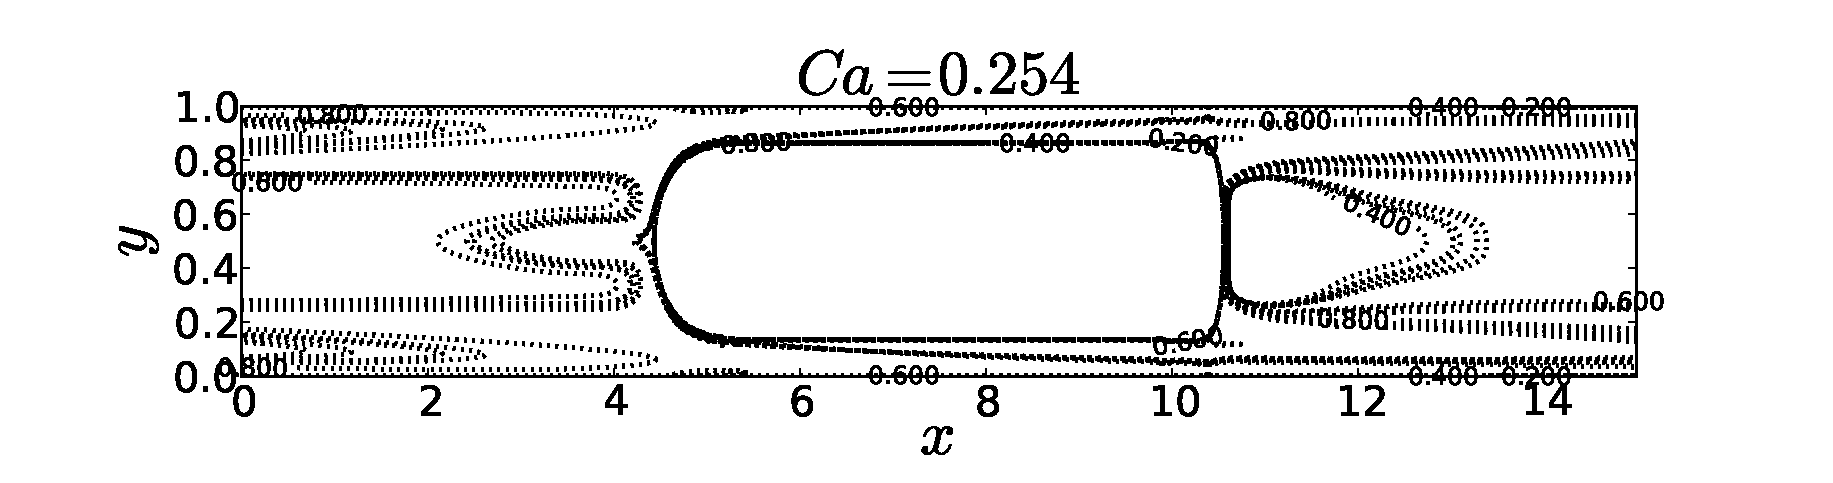
\includegraphics[height=0.25\textwidth]{contourlines_scale_ca054.eps}\\
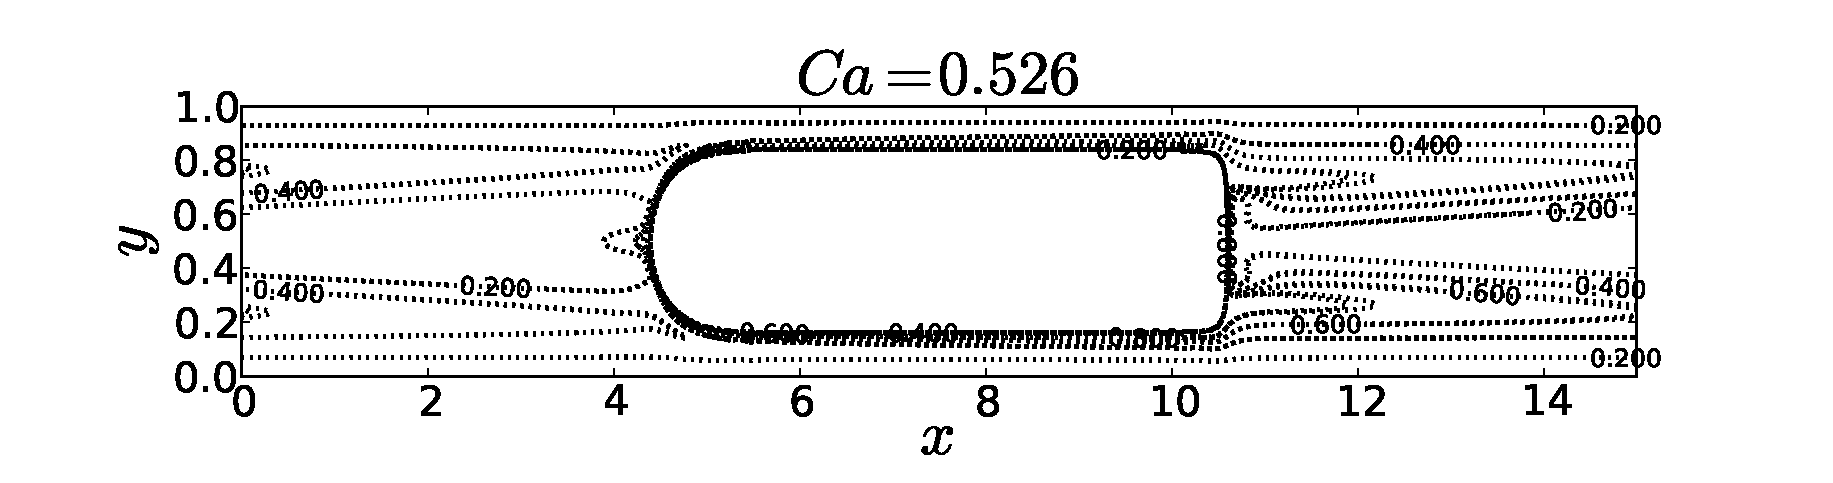
\includegraphics[height=0.25\textwidth]{contourlines_scale_ca026.eps}\\
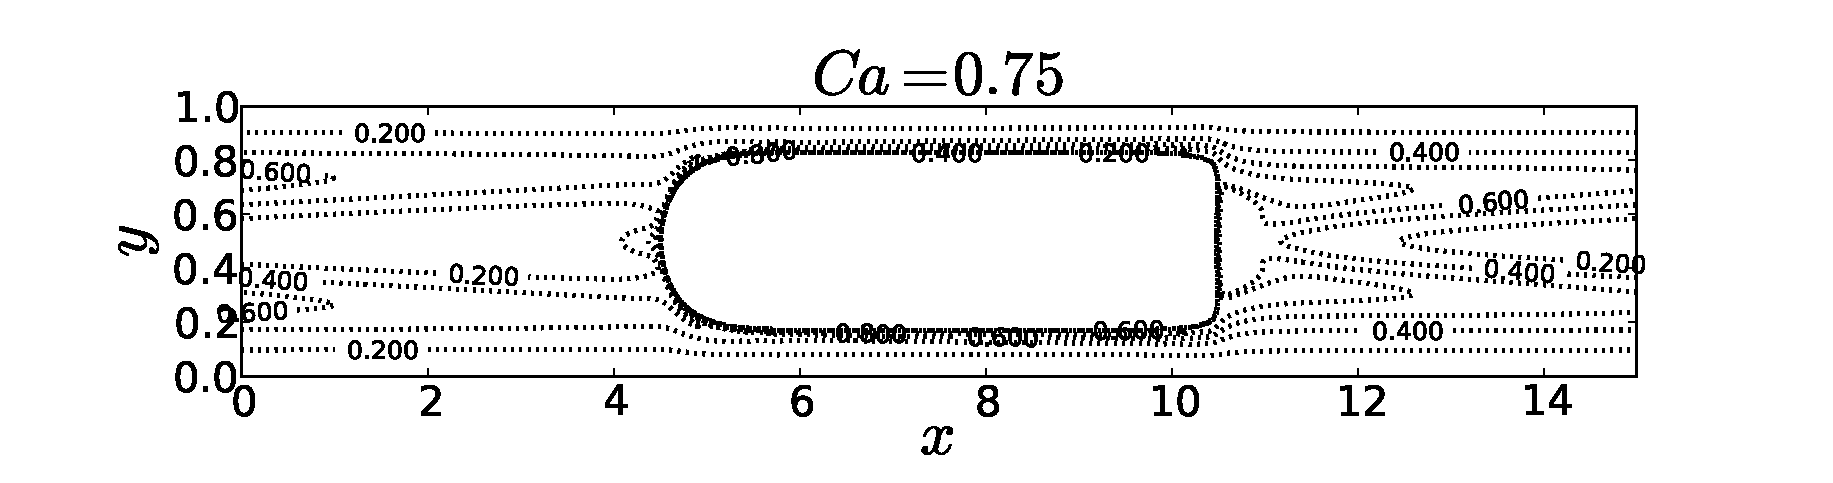
\includegraphics[height=0.25\textwidth]{contourlines_scale_ca05.eps}\\
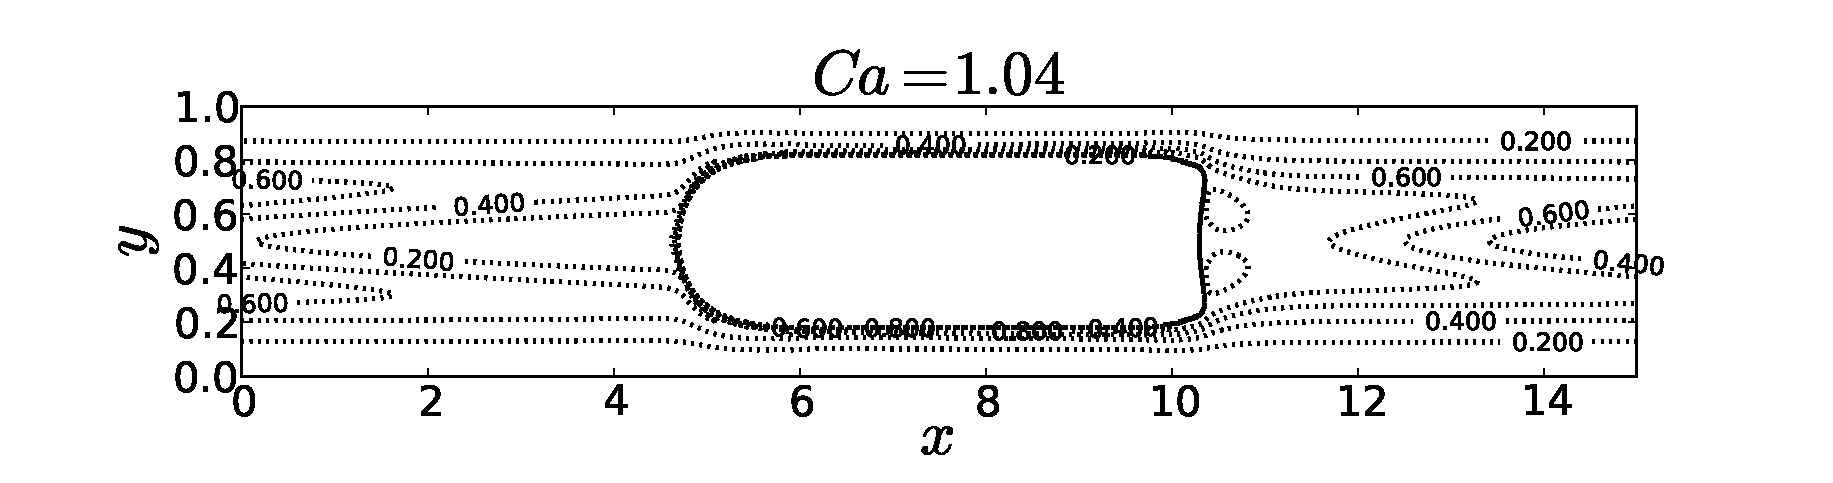
\includegraphics[height=0.25\textwidth]{contourlines_scale_ca14.eps}\\
\caption{Concentration contour profiles for velocity scalings as identified in Table
\ref{table:scaling:peclet} (top to bottom:
$Ca=0.097,0.254,0.526,0.750,1.040$). Lines correspond to
all different scales indicated in Table
\ref{table:scaling:peclet} (top to bottom: 6 scalings, 5 scalings, 2 scalings, 1 scaling, 1 scaling). Some lines are indistinguishable showing that simulations with velocity scalings are consistent.  \label{fig:contours:scaling:peclet}}
\end{figure}

\subsection{Average concentration results}
\label{main:results:periodic}
In this section we will examine the case where the volume averaged concentration over
 time is used as the characteristic concentration. To calculate the volumetric mass transfer coefficient we used Eq. \ref{theor:one:concentration:time}.
%\beqal
%&\vol t \frac{\ububble}{\ugas+\uliq}=\ln\frac{\cstar}{\cstar-\langle C(t) \rangle}\\
%&\vol \frac{\lunit}{\ugas+\uliq}=\frac{\lunit}{\ububble t} \ln \frac{C^*}{C^*-\langle C(t)
%\rangle},\\
%\feqal
%where $\langle C(t) \rangle$ is the average concentration in the liquid domain.
Results for the coefficient $\vol \frac{\ububble}{\ugas+\uliq}$ are shown in Fig.
\ref{fig:aver:conc:different:capillaries} for different Peclet numbers and velocity scalings
indicated in Table \ref{table:scaling:peclet}. When the average concentration gets
close to $\cstar=1$ then Eq. \ref{theor:one:concentration:time} gives inadequate results due to
 accuracy of the logarithmic function evaluation. This is the reason that curves in Fig. \ref{fig:aver:conc:different:capillaries}
 tend to shoot up for long times.
 %Fig. \ref{fig:aver:conc:different:capillaries:time} presents
%the volumetric mass transfer coefficient as a function of number of iterations. 
Due to velocity scaling
each simulation has a different physical time step. Thus, we normalized time such that it represents a number of unit cell lengths which the bubble will pass, i.e. 
$N_{\text{cell\,units}}=\frac{\text{scale}\cdot \ububble\cdot N_{\mathrm{iter}}}{\lunit}$.  Fig.
\ref{fig:aver:conc:different:capillaries} shows the volumetric mass transfer
dependency against the distance in unit cell length. One can see in Table
\ref{table:steady:state:average} that for different Peclet numbers different time (number of unit
cells) is required to achieve  steady state. For example, for
larger Peclet numbers fewer iterations are required to achieve the steady state condition. 

Overall one obtains  steady state volumetric mass transfer coefficients for
periodic boundaries simulations if the following conditions are fulfilled:
\begin{description}
\item[I] Scaling is performed as $U_{max}=\mathrm{scale}\cdot\ububble\leq 0.1$.
\item[II] The larger the Peclet number, the fewer iterations are required. One can extrapolate data from Table
\ref{table:steady:state:average}, say $L_{\mathrm{steady}}$, and estimate the  number of
iterations to reach the steady-state as $\mathrm{scale}\cdot \ububble\cdot N_{\mathrm{iter}}\leq L_{\mathrm{steady}}$. 
\end{description}
%Also, Table \ref{table:steady:state:average} shows
%the achieved steady state volumetric mass transfer coefficient. 
%\begin{figure}[htb!]
%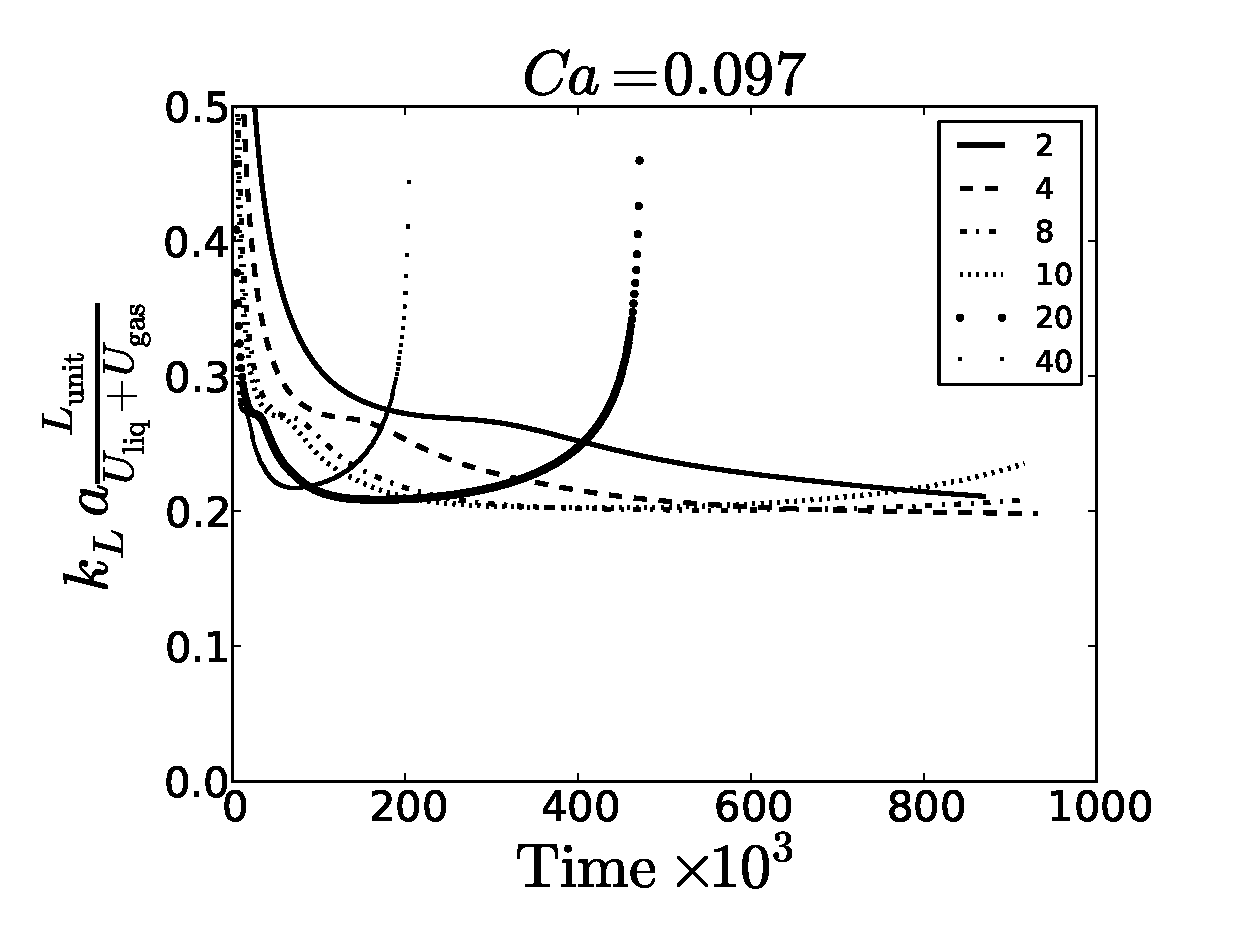
\includegraphics[width=0.5\textwidth]{Figures/aver_conc_scale_ca_time097.eps}
%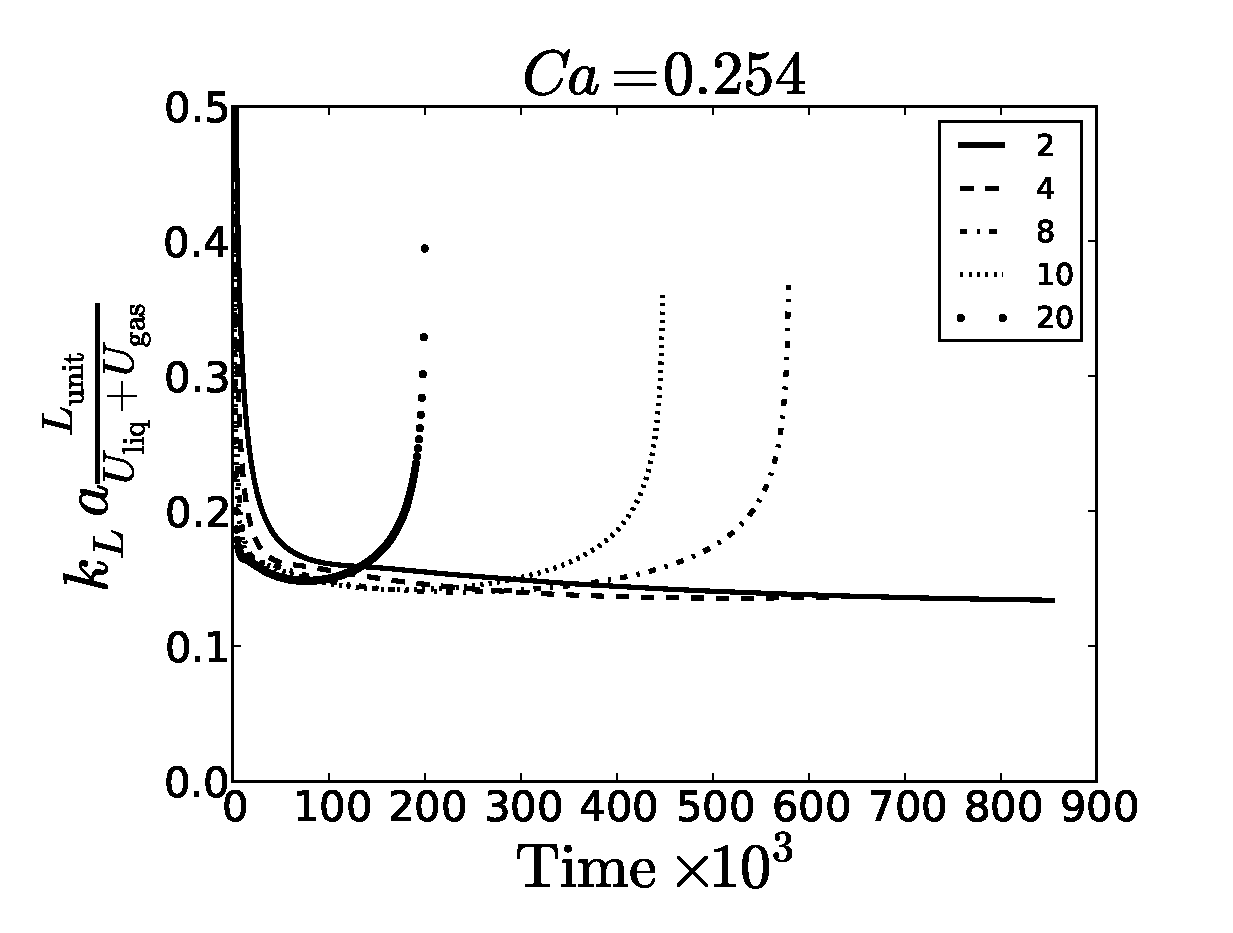
\includegraphics[width=0.5\textwidth]{Figures/aver_conc_scale_ca_time054.eps}\\
%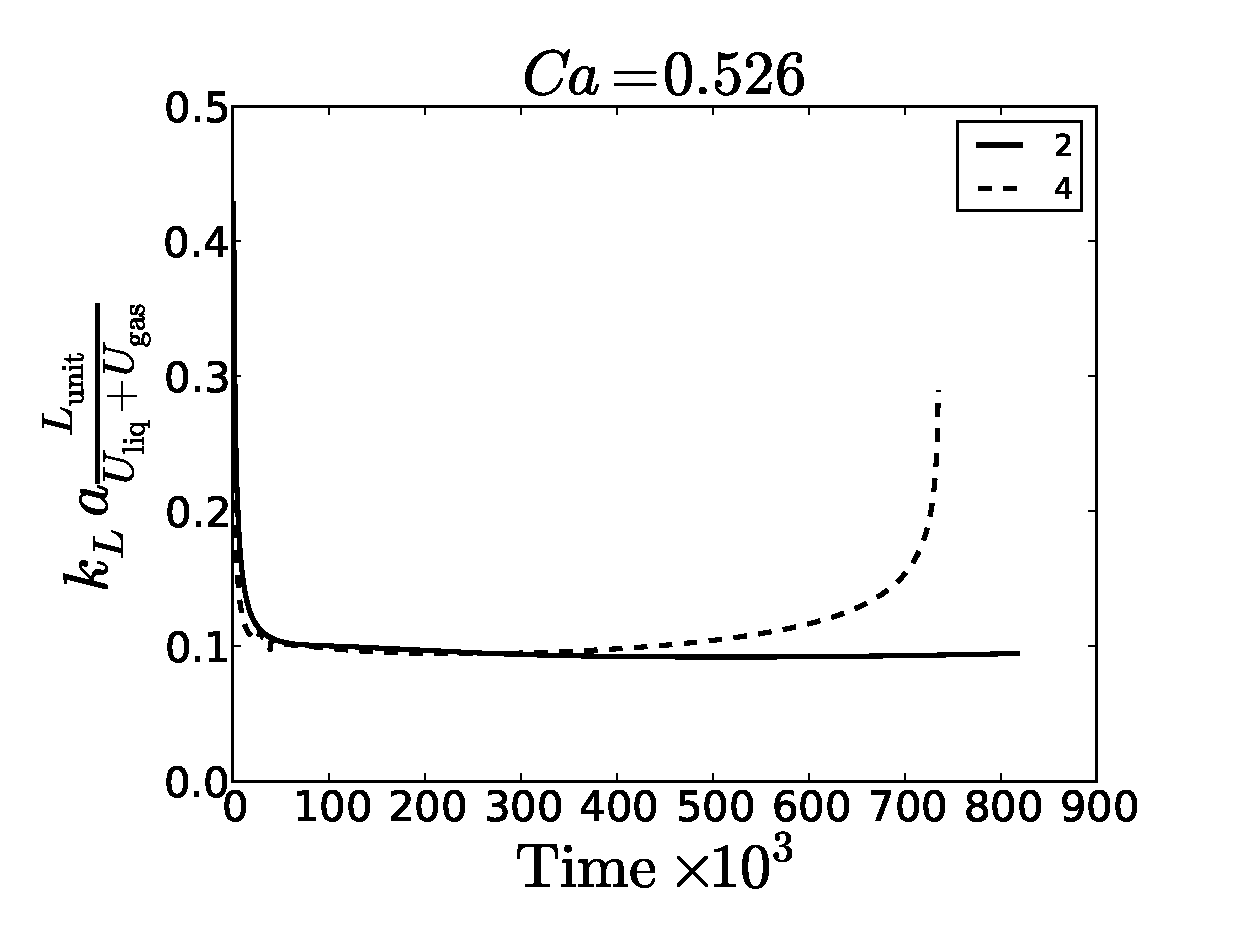
\includegraphics[width=0.5\textwidth]{Figures/aver_conc_scale_ca_time026.eps}
%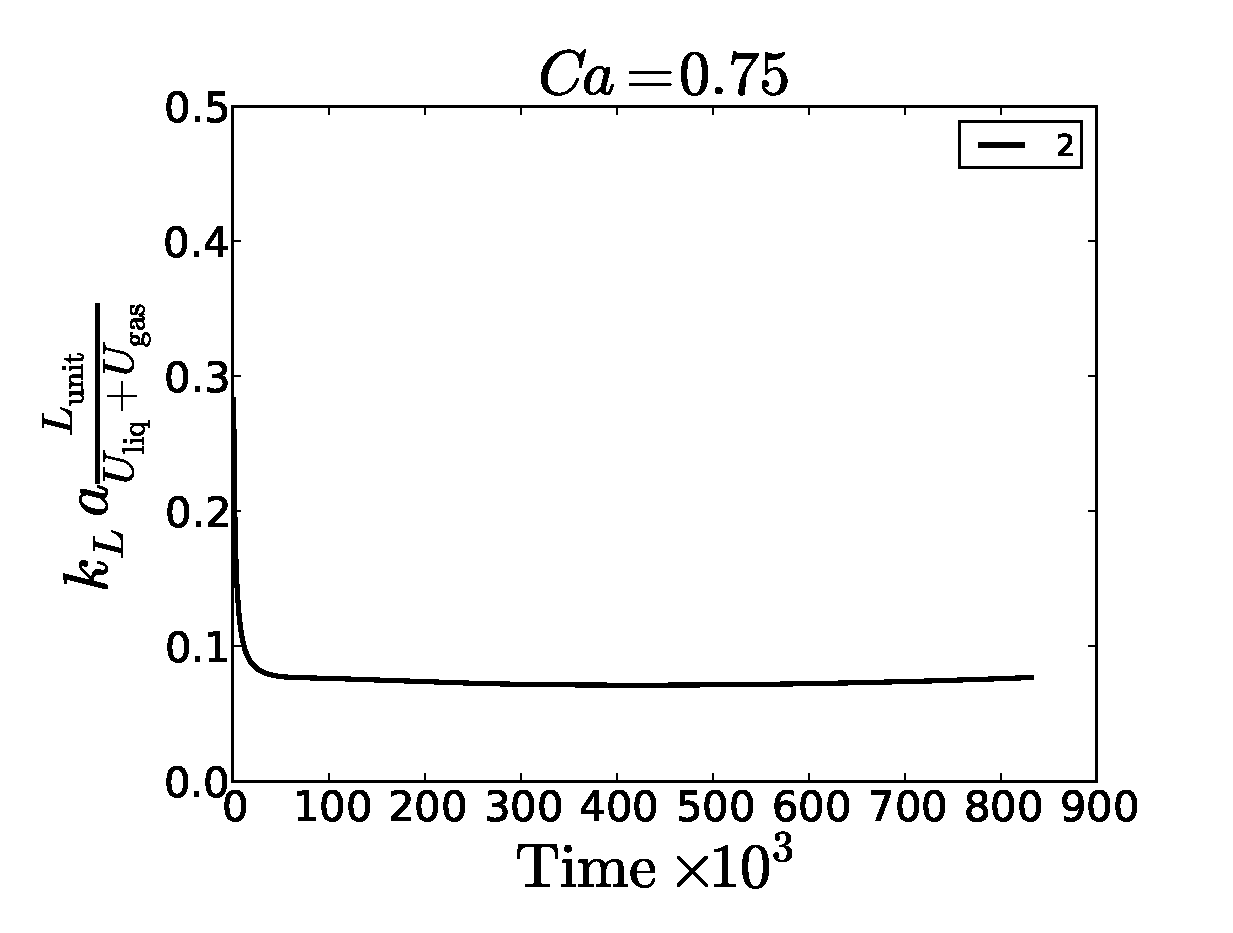
\includegraphics[width=0.5\textwidth]{Figures/aver_conc_scale_ca_time05.eps}\\
%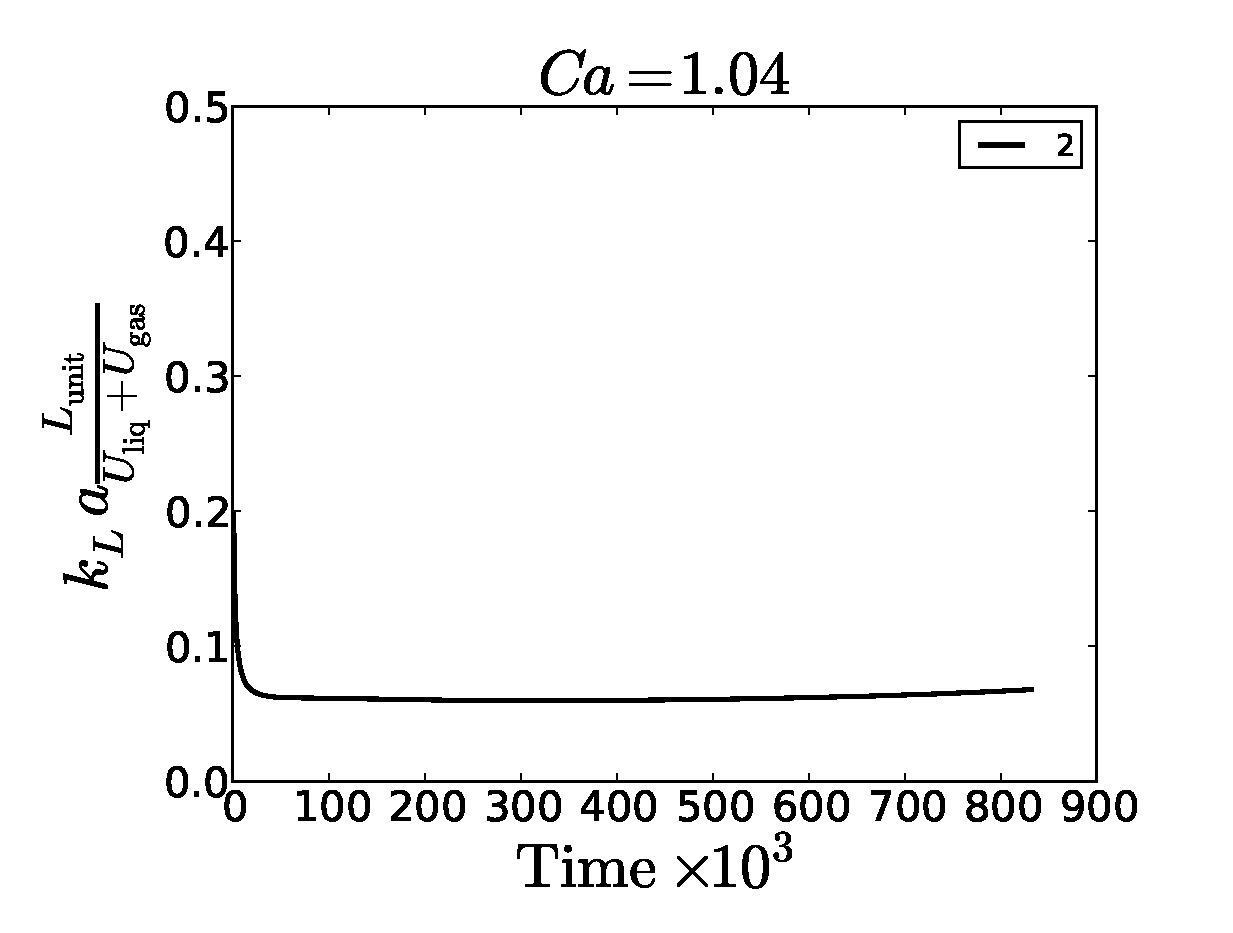
\includegraphics[width=0.5\textwidth]{Figures/aver_conc_scale_ca_time14.eps}
%\caption{Calculated volumetric mass transfer coefficient for different capillaries and scales
%against time. One can see
%that all curves have the same minimum corresponding to the volumetric mass transfer coefficient.
%Some simulations show the volumetric mass transfer coefficient going up due to the average
%concentration being close to $\cstar$. All of them show an excellent agreement. Note, that with the
%velocity scaling one can reduce the amount of calculations drastically. However, one needs to be attentive
%because with large velocity scaling average concentration can quickly approach $\cstar$, thus
%getting an infinite volumetric mass transfer coefficient.
%\label{fig:aver:conc:different:capillaries:time}}
%\end{figure}
\begin{figure}[htb!]
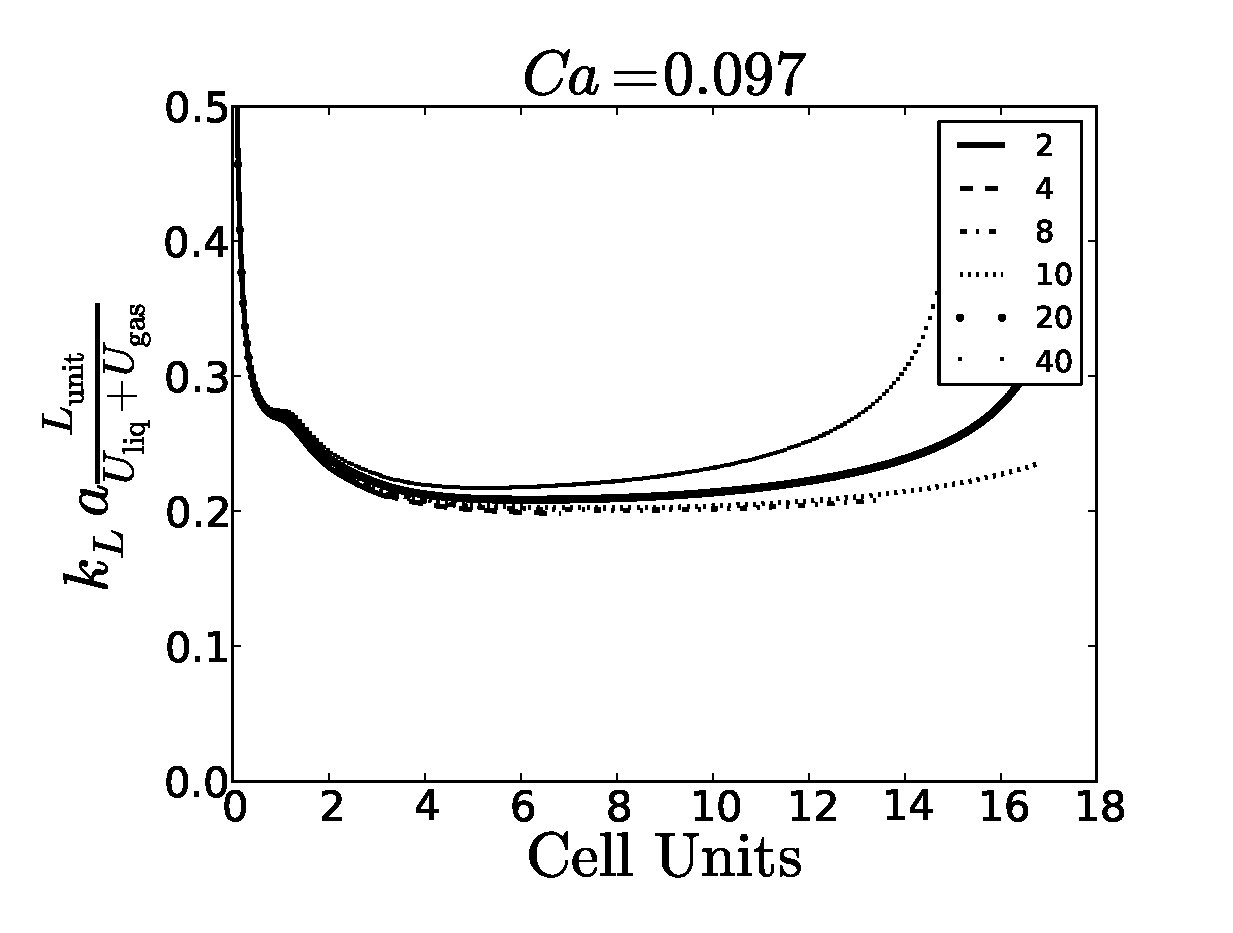
\includegraphics[width=0.5\textwidth]{aver_conc_scale_ca097.eps}
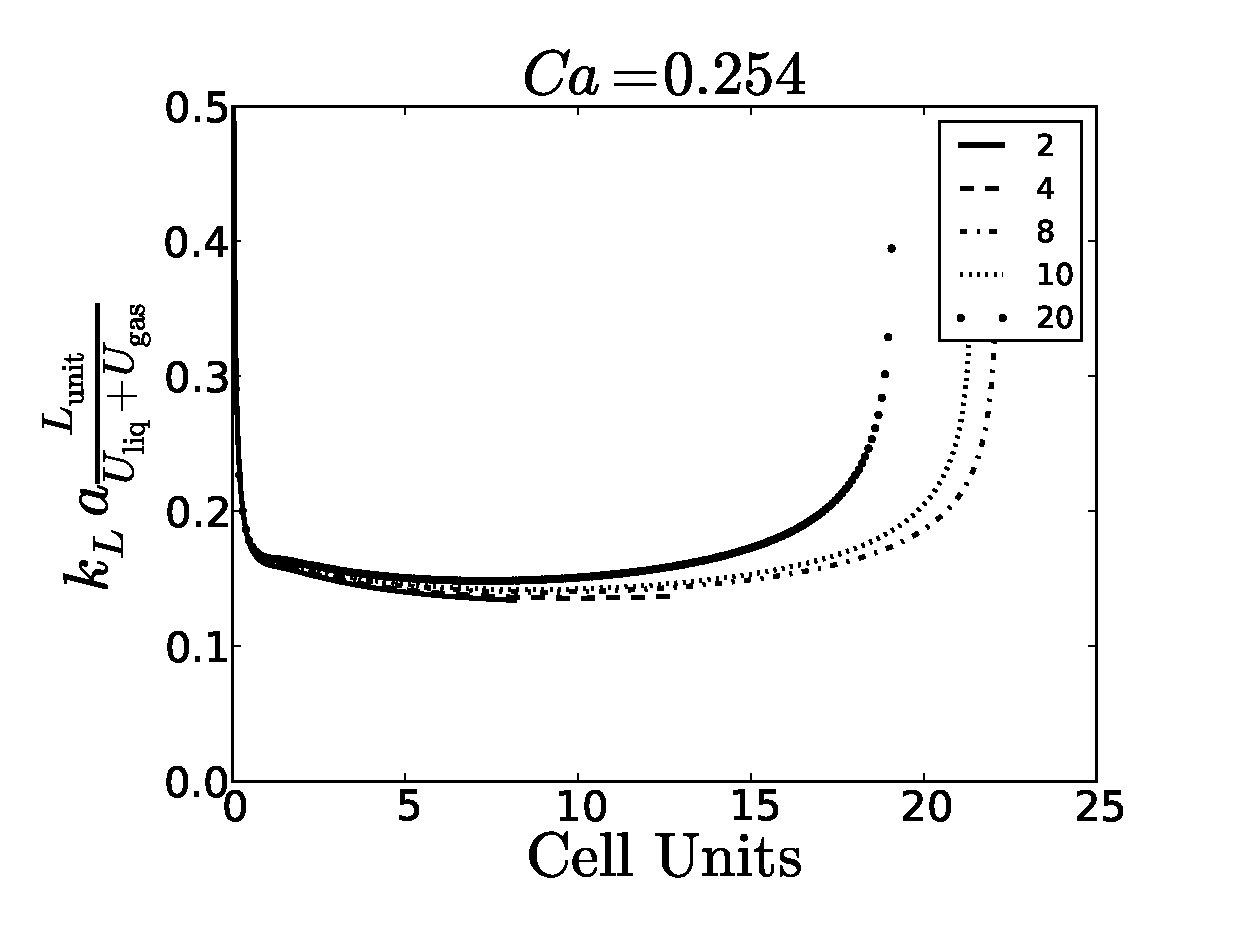
\includegraphics[width=0.5\textwidth]{aver_conc_scale_ca054.eps}\\
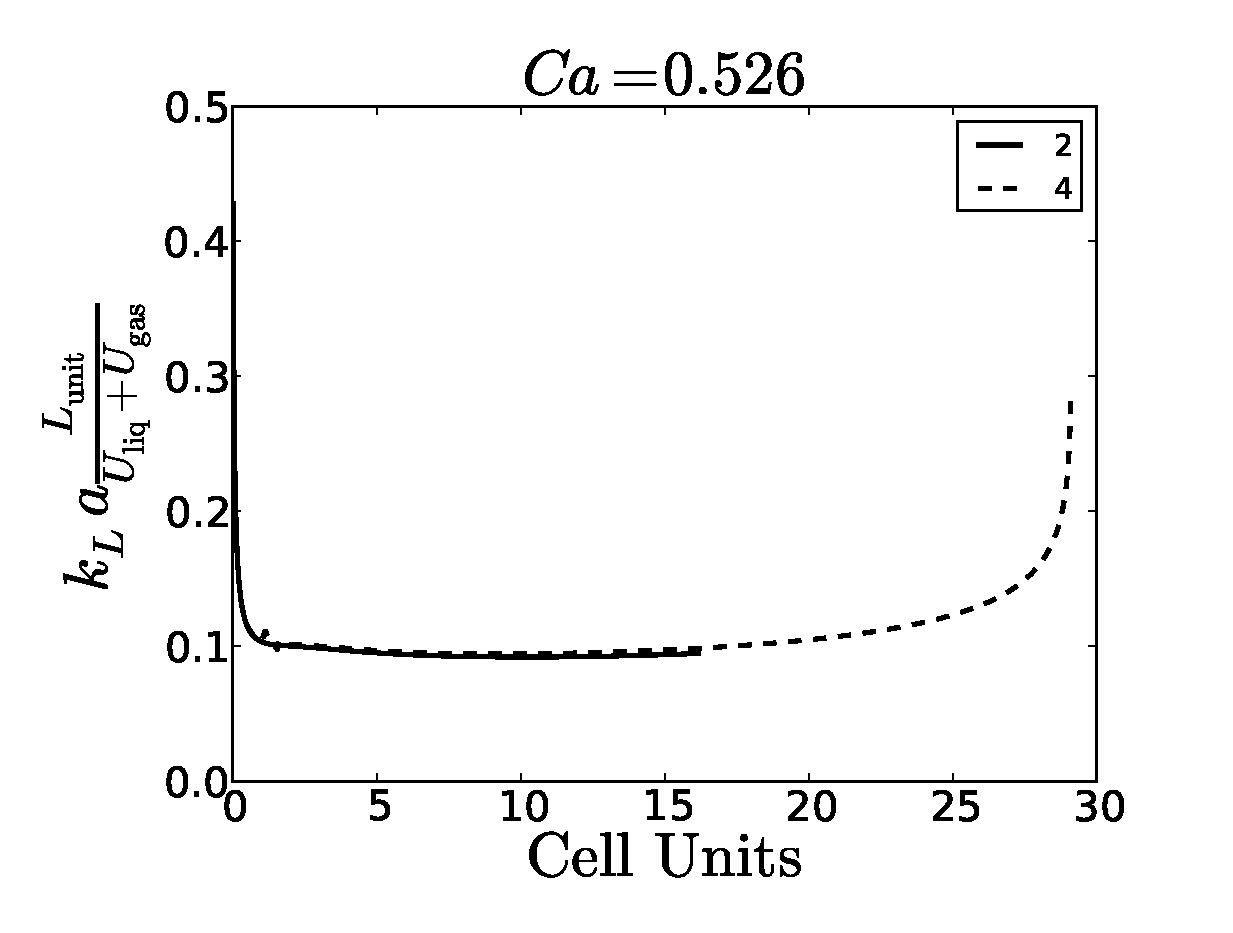
\includegraphics[width=0.5\textwidth]{aver_conc_scale_ca026.eps}
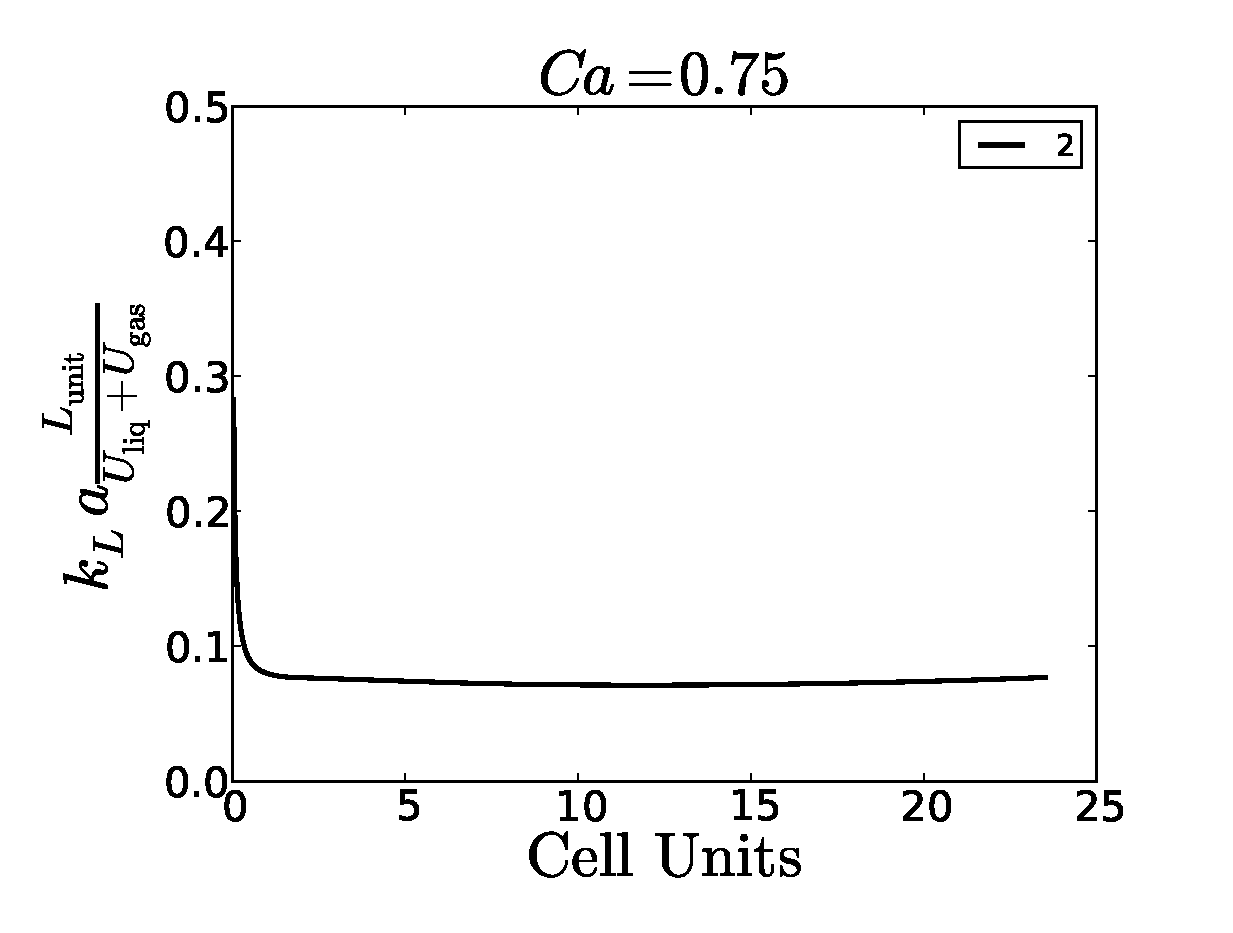
\includegraphics[width=0.5\textwidth]{aver_conc_scale_ca05.eps}\\
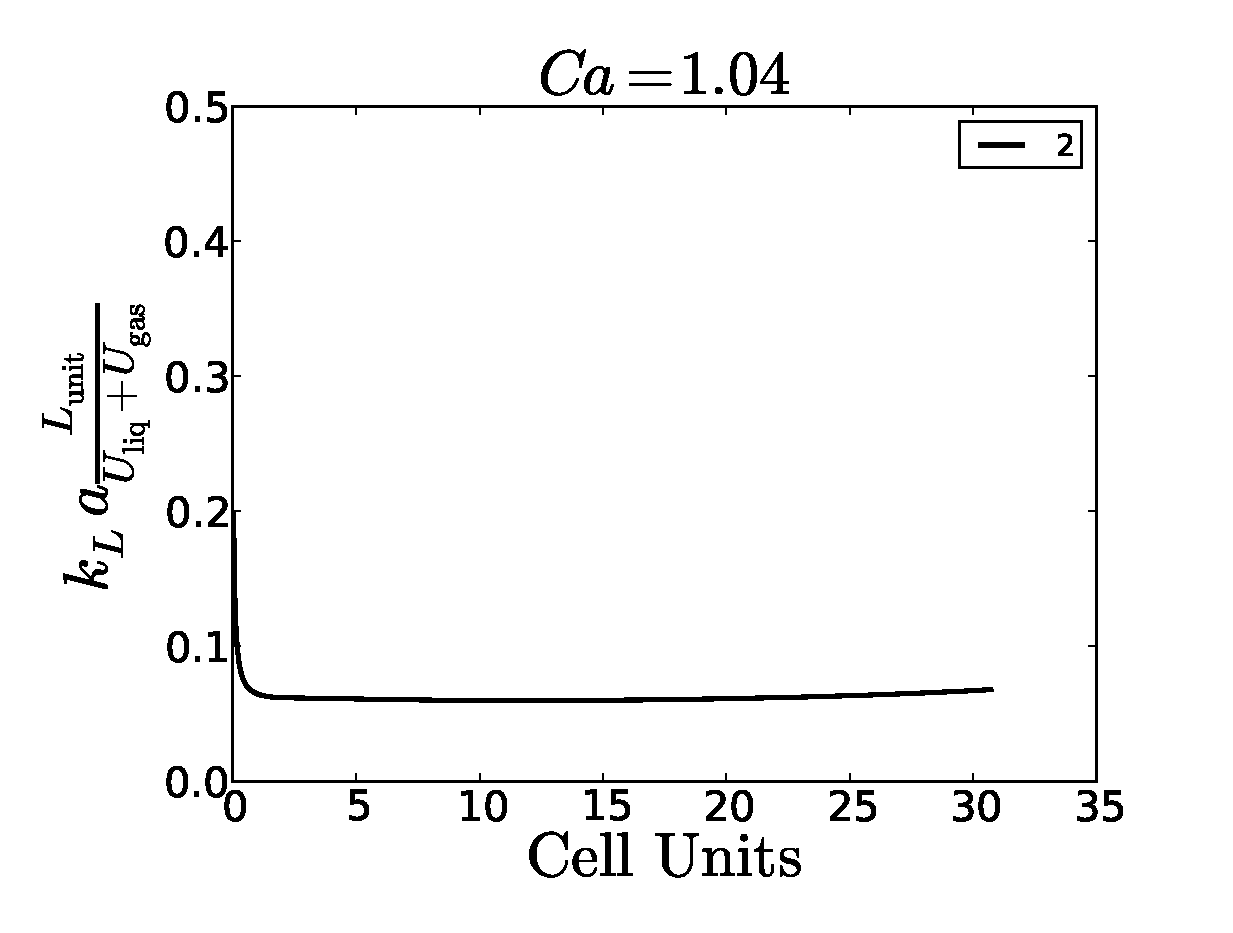
\includegraphics[width=0.5\textwidth]{aver_conc_scale_ca14.eps}
\caption{Volumetric mass transfer coefficient for different capillary numbers and scales against the
bubble travel distance in the laboratory frame. ''Cell Units`` axis refers to the physical
distance of how many unit cells the bubble travels until the steady state is reached. A legend is provided for velocity scalings. All of them show a good agreement.One can see an abnormal rise of the mass transfer coefficient when the average concentration is close to $\cstar$ due to the logarithmic function evaluation.  Table
\ref{table:steady:state:average}
summarizes results presented here.  \label{fig:aver:conc:different:capillaries}}
\end{figure}
\begin{table}[htb!]
\begin{tabularx}{\textwidth}{|X|X|X|X|}
\hline
$Ca$    &$Pe$     &$L_{\mathrm{steady}}/\lunit$& $\volnondim$ \\
\hline
$0.097$ &$1313$  &$7$&$0.21$  \\ 
$0.254$ &$3414$  &$6$&$0.14$  \\ 
$0.526$ &$7092$  &$3$&$0.095$ \\
$0.750$ &$10125$ &$3$&$0.074$ \\
$1.040$ &$14041$ &$2$&$0.0601$\\
\hline
\end{tabularx}
\caption{The distance which a bubble propagates when the
steady-state condition is achieved. 
%One can see that increasing Peclet number helps to achieve the steady state faster.
\label{table:steady:state:average}}
\end{table}

\subsection{Periodic boundaries with the inlet/outlet characteristic concentration}
\label{results:periodic:inlet:outlet} 
The volumetric mass transfer coefficient
was calculated using Eq. \ref{theor:one:concentration:time} with the
characteristic concentration being the inlet/outlet flux averaged concentration
as used by \citet{vanbaten-circular}. One can see in Fig.
\ref{fig:volumetric:char:concentration:vanbaten} that the calculated volumetric mass
transfer behave differently from the domain averaged  volumetric mass
transfer coefficient. For example, for small capillary numbers, i.e.
$Ca=0.097,0.254,0.526$ the values are overpredicted
($\volnondim=0.3,0.25,0.1$). When the velocity pattern changes from having
a vortex in front of
the bubble to not having it,  i.e. $Ca=0.75,1.04$ the calculated values
are underpredicted compared to estimates based on volume-averaged concentration, i.e. $\volnondim=0.06,0.04$. As we will see later, the domain-averaged characteristic concentration produces proper mass transfer coefficients. 
\begin{figure}[htb!]
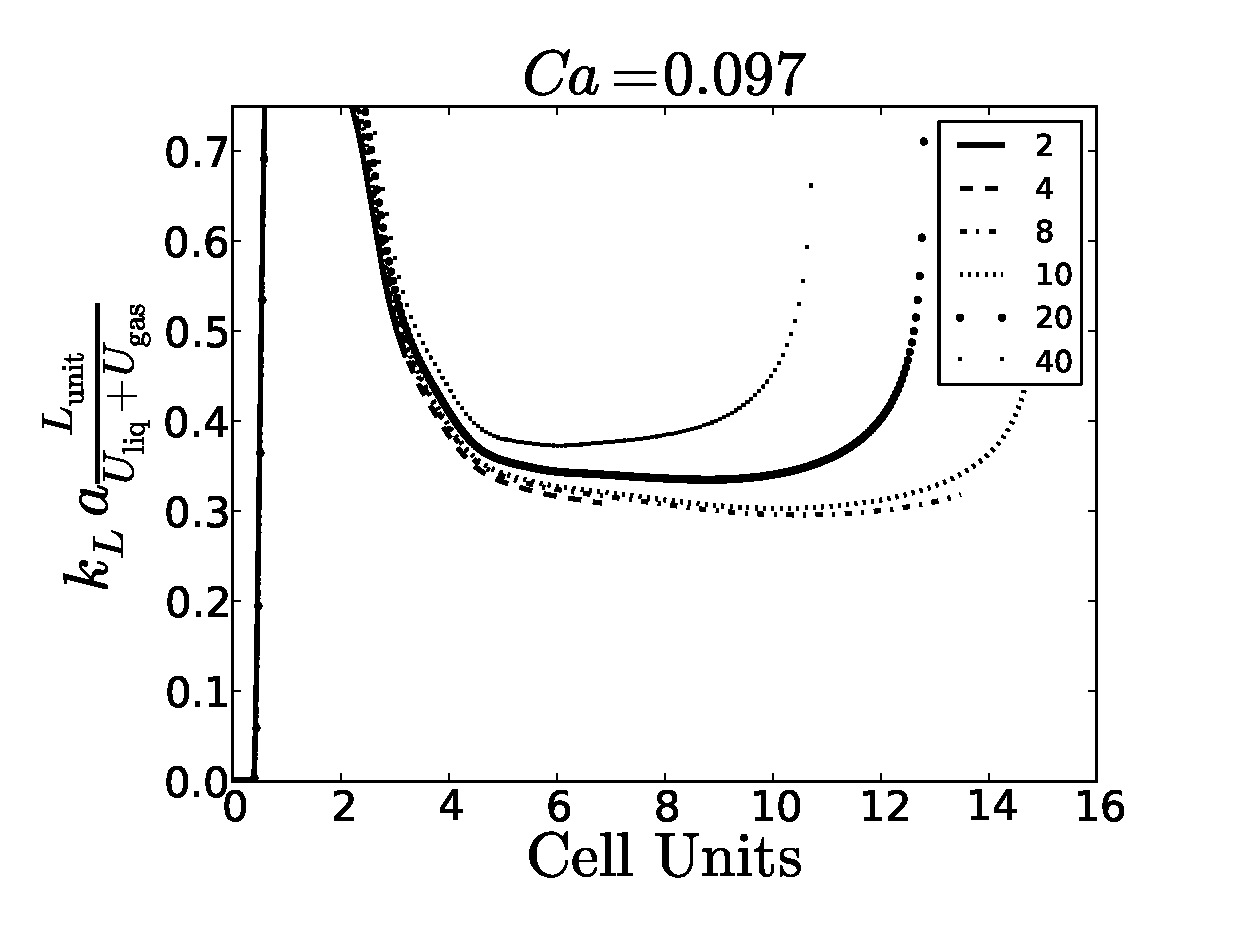
\includegraphics[width=0.5\textwidth]{aver_vanbaten_scale_ca097.eps}
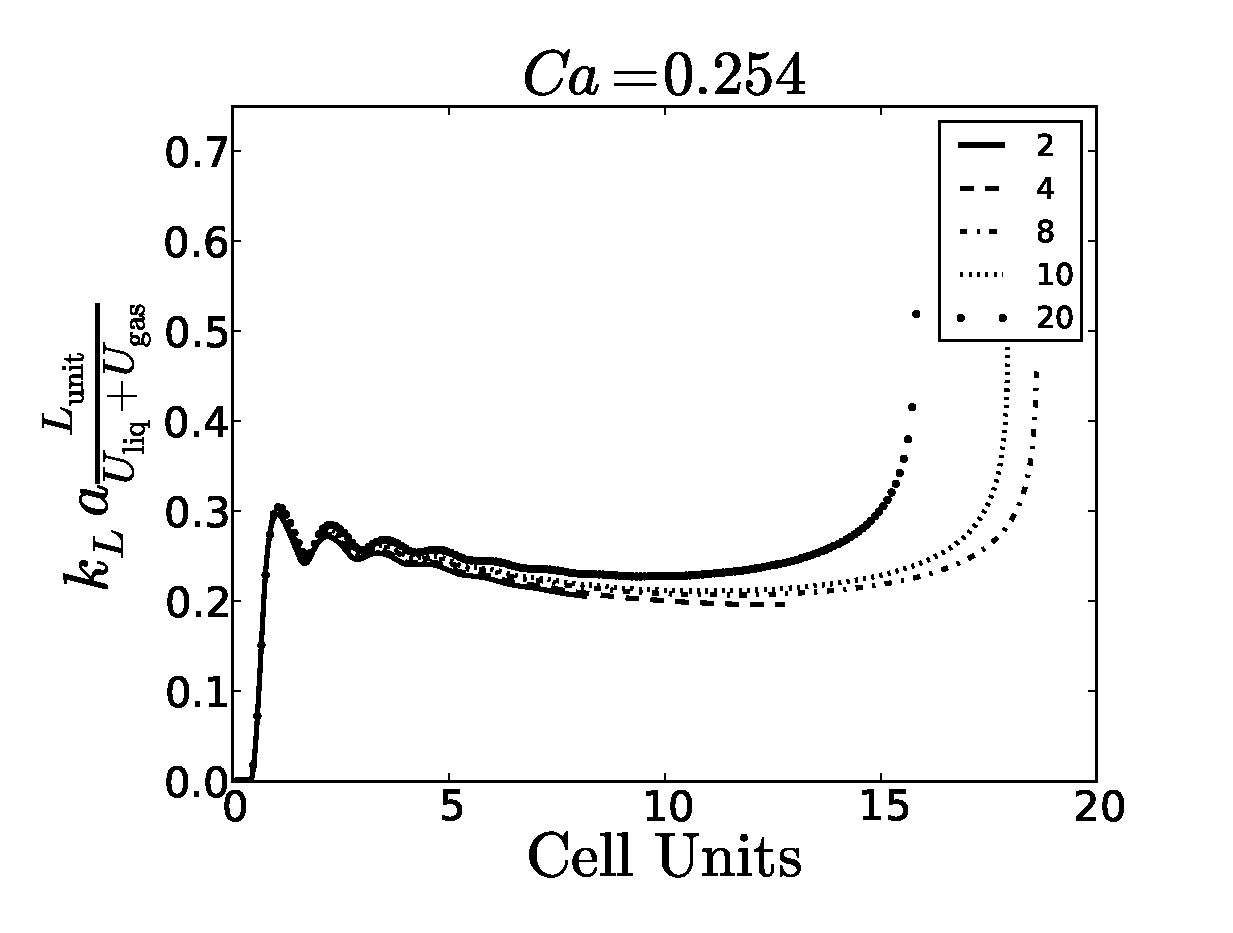
\includegraphics[width=0.5\textwidth]{aver_vanbaten_scale_ca054.eps}\\
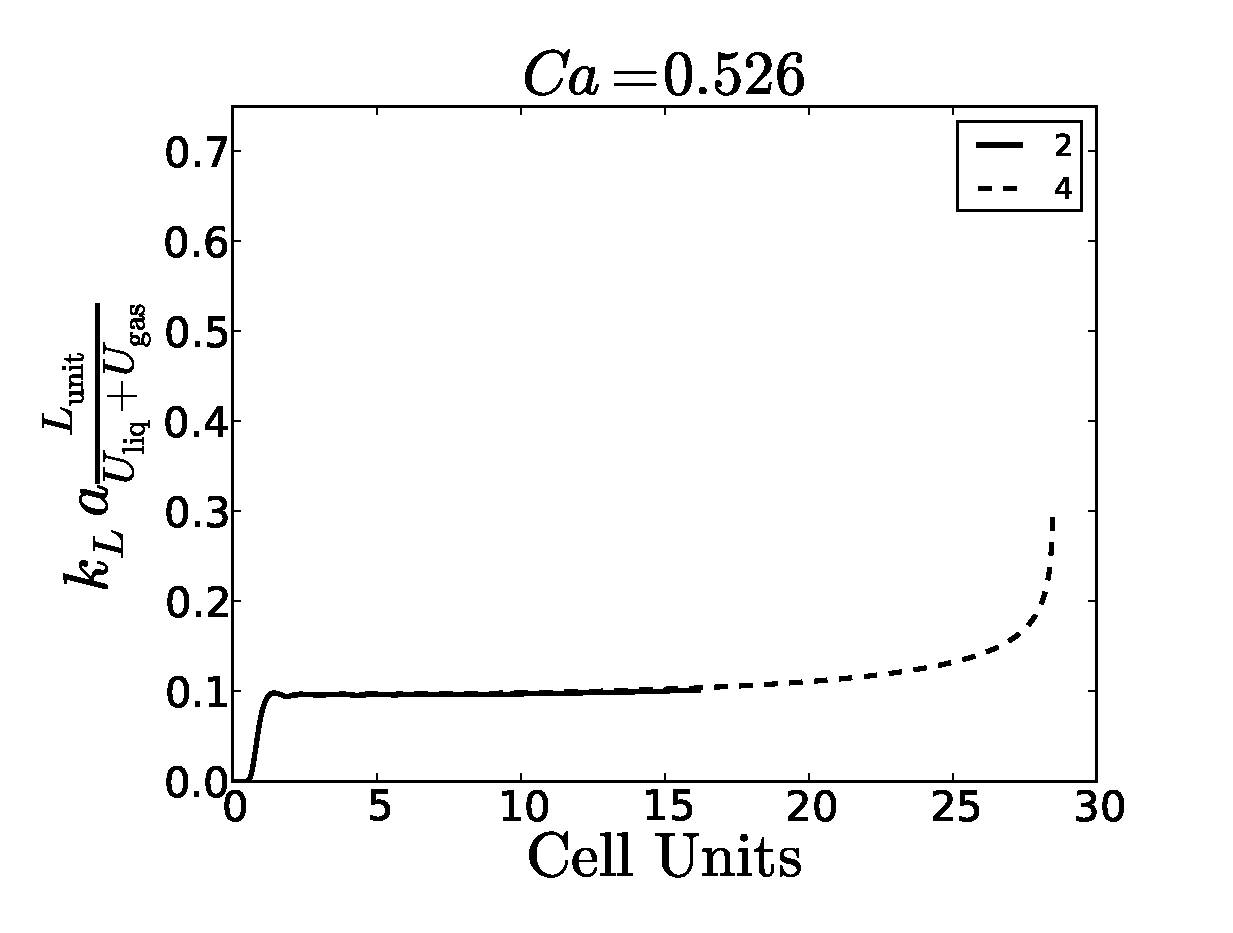
\includegraphics[width=0.5\textwidth]{aver_vanbaten_scale_ca026.eps}
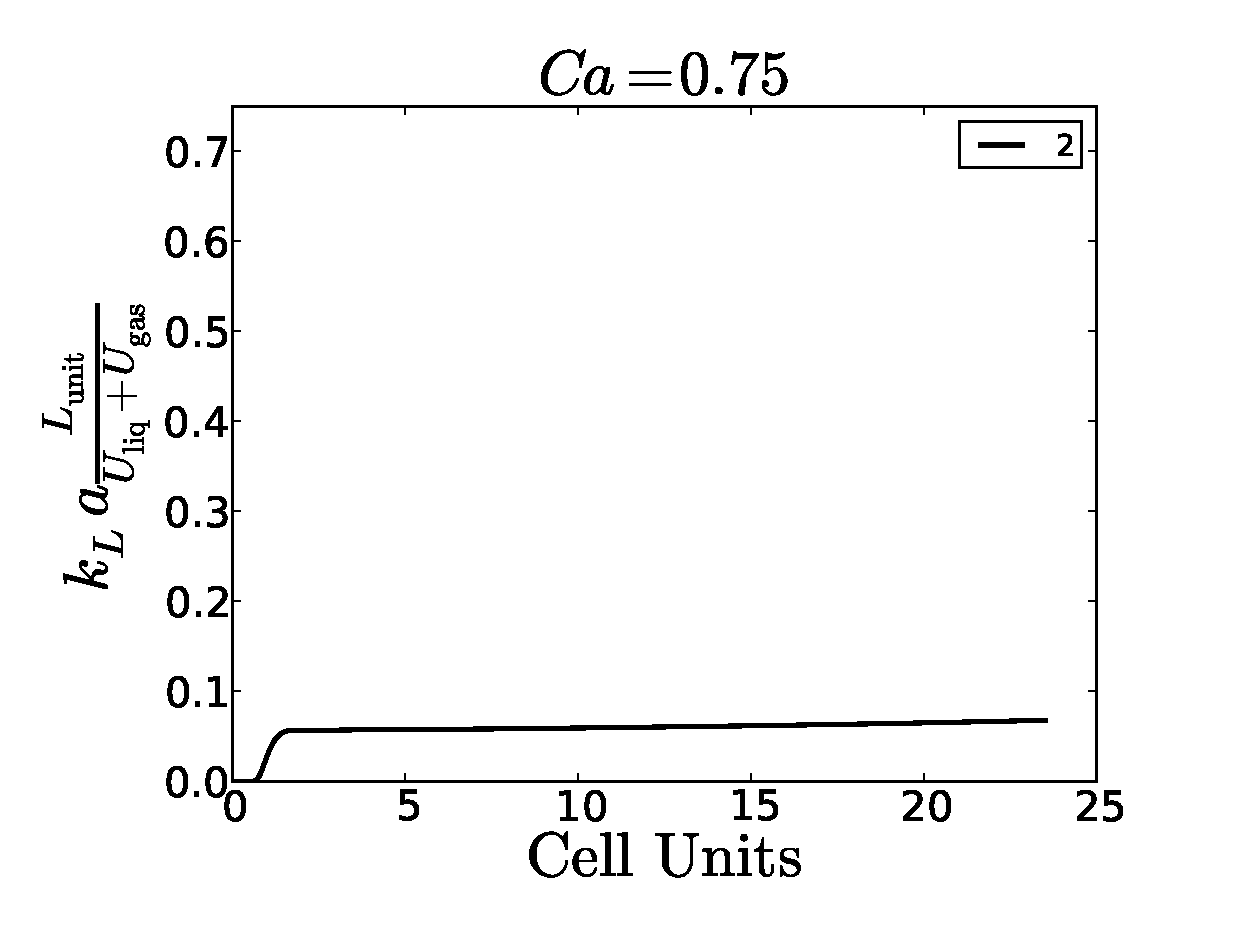
\includegraphics[width=0.5\textwidth]{aver_vanbaten_scale_ca05.eps}\\
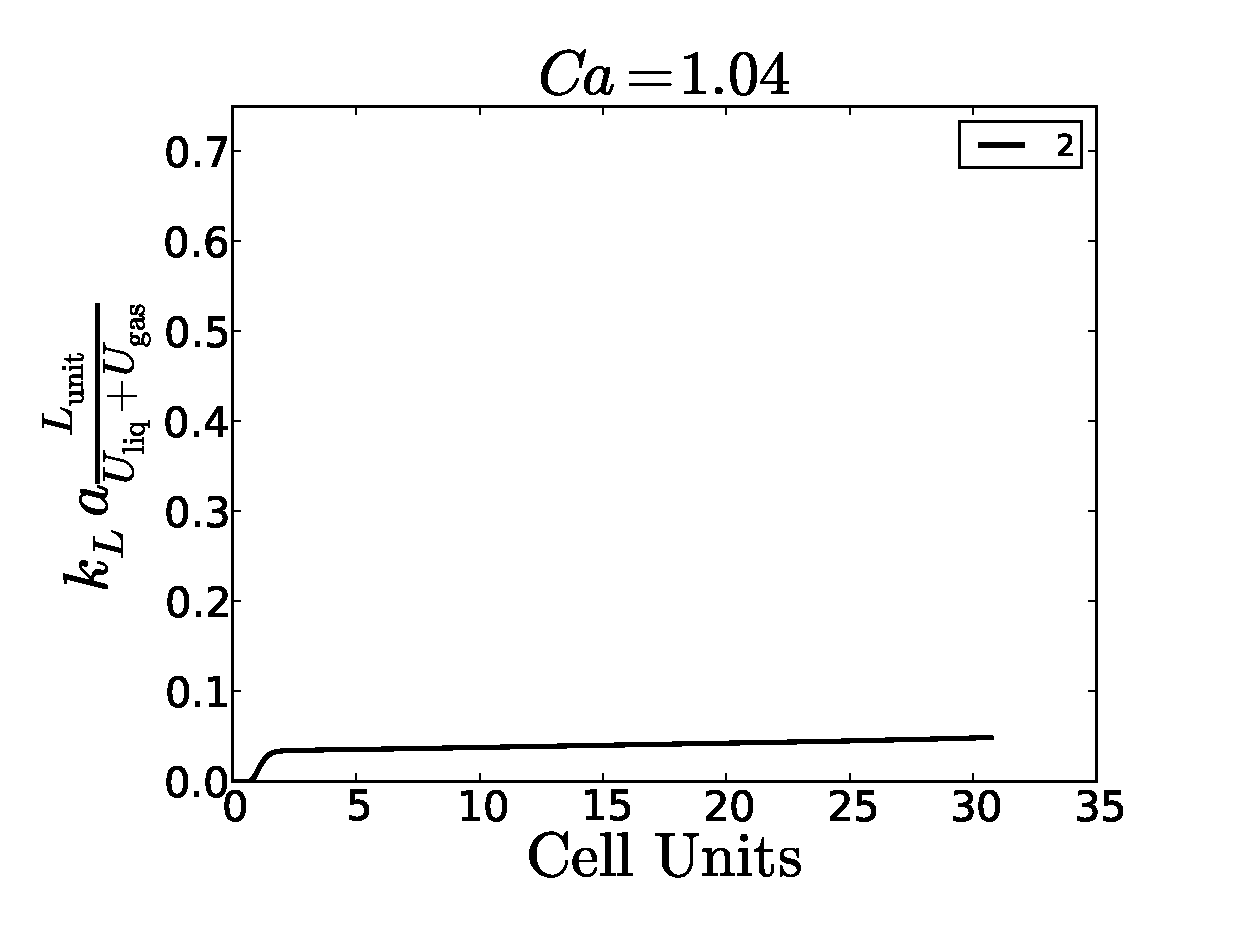
\includegraphics[width=0.5\textwidth]{aver_vanbaten_scale_ca14.eps}
\caption{The volumetric mass transfer coefficient
with the characteristic concentration based on
the inlet/outlet flux averaged concentration as
in \cite{vanbaten-circular}. One can see that depending on the velocity pattern,
 the values are either overpredicted or underpredicted
in comparison to values specified in Table \ref{table:steady:state:average} 
\label{fig:volumetric:char:concentration:vanbaten}}
\end{figure}

\subsection{Van Baten and Krishna formulation}
\label{results:vanbaten}
The \citet{vanbaten-circular} formulation, Eq. \ref{eq:vanbaten:formulation}, is calculated as
the change of mass in the domain divided by the time difference. We examined two
approaches:  the characteristic concentration taken to be as the domain average
and as the flux-averaged input/output concentration. The latter case
corresponds to  \cite{vanbaten-circular}. The results are presented in
Fig. \ref{fig:vanbaten} for $Ca=0.097$ and $Ca=1.04$. One can see that the
inlet/outlet flux averaged concentration is inconsistent. The
reason that \citet{vanbaten-circular} obtained the mass transfer coefficient
close to the analytical estimation is that the liquid slug is well mixed ($Ca<0.1$ which is below the range studied here) so that
the averaged concentration is close to the inlet/outlet concentration.

However, results for the domain-averaged concentration using the approach of \citeauthor{vanbaten-circular} are close to simulation results in Section
\ref{main:results:periodic}. %for the volumetric mass transfer coefficient measured with the domain
%averaged concentration in the whole range of capillary numbers. 
Note that for $Ca=0.097$ the obtained mass transfer coefficient value is $10\%$ 
lower than the value in Section \ref{main:results:periodic}. However, as will
be shown later the obtained volumetric mass transfer coefficient for
$Ca=0.0097$ has the same value as for the simulations of a few unit cells.
Therefore the approach of \citet{vanbaten-circular} produces  accurate results but if the characteristic concentration is the volume-averaged concentration (not the inlet/outlet flux-averaged concentration used in the original work). From the computational point of view, it also requires the concentration fields in time and space to calculate the mass change in time and the averaged domain
characteristic concentration.
% only for velocity patterns related to larger
%Capillary numbers, i.e. $Ca\geq0.7$. 
\begin{figure}
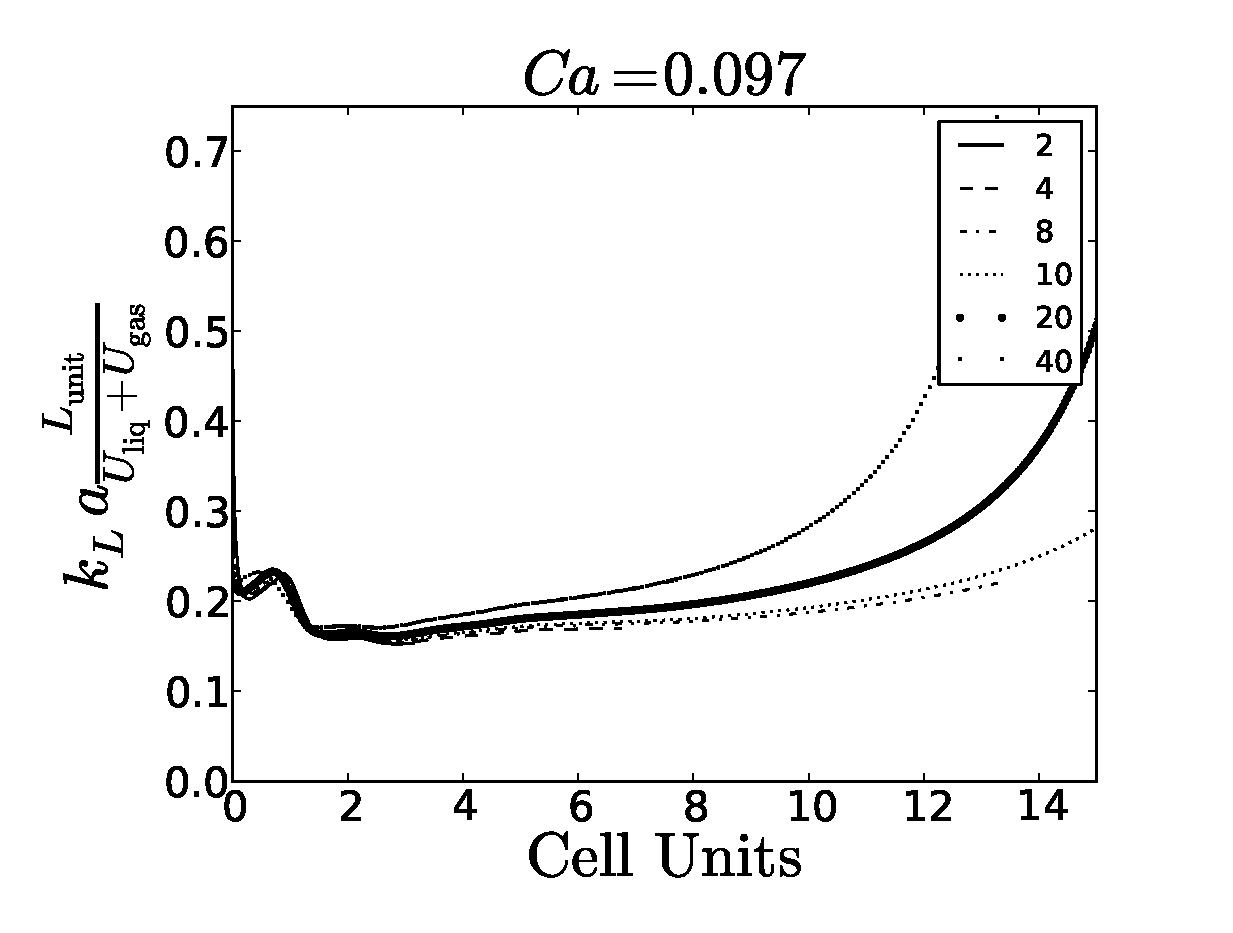
\includegraphics[width=0.5\textwidth]{vanbaten_aver_scale_ca097.eps}
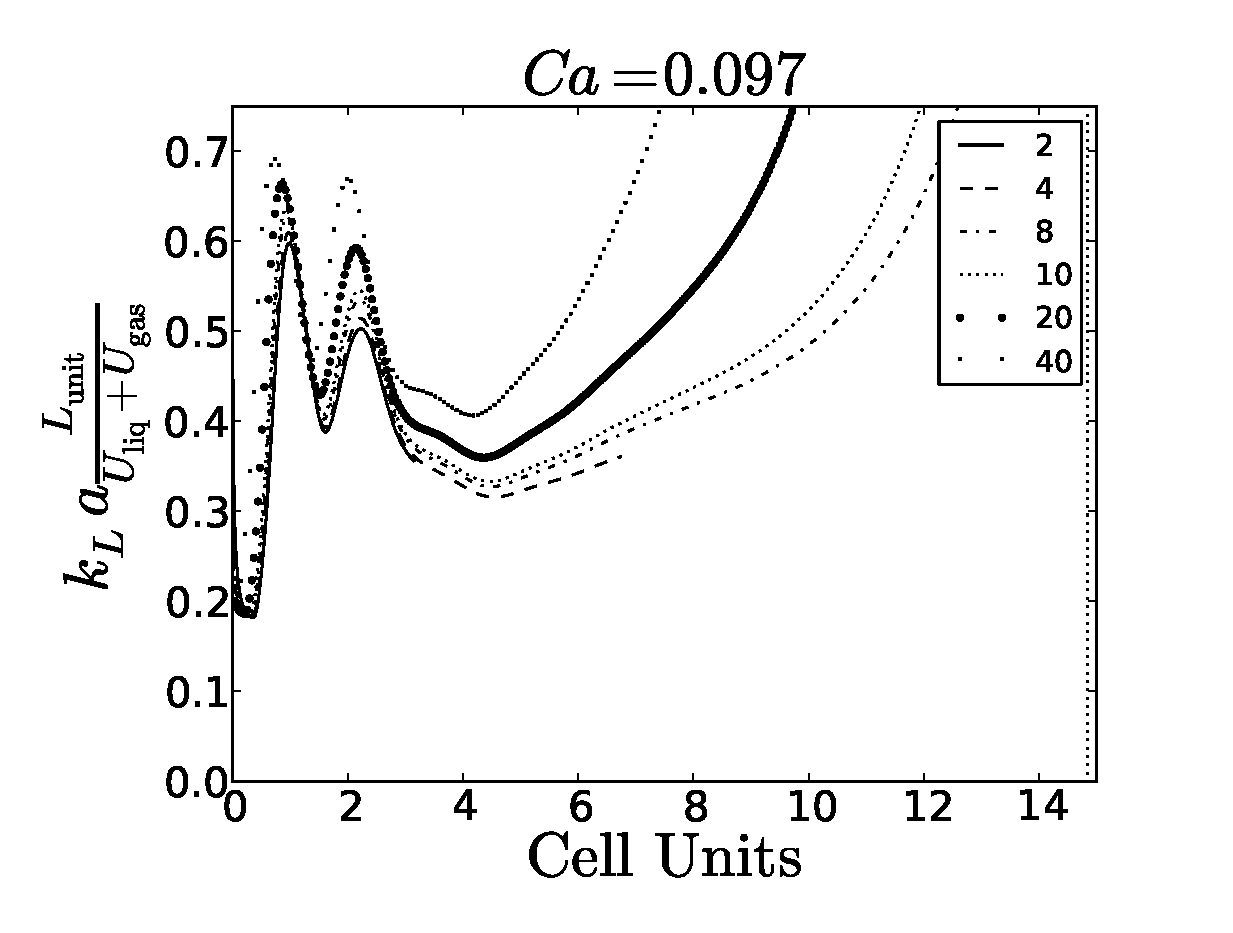
\includegraphics[width=0.5\textwidth]{vanbaten_full_scale_ca097.eps}\\
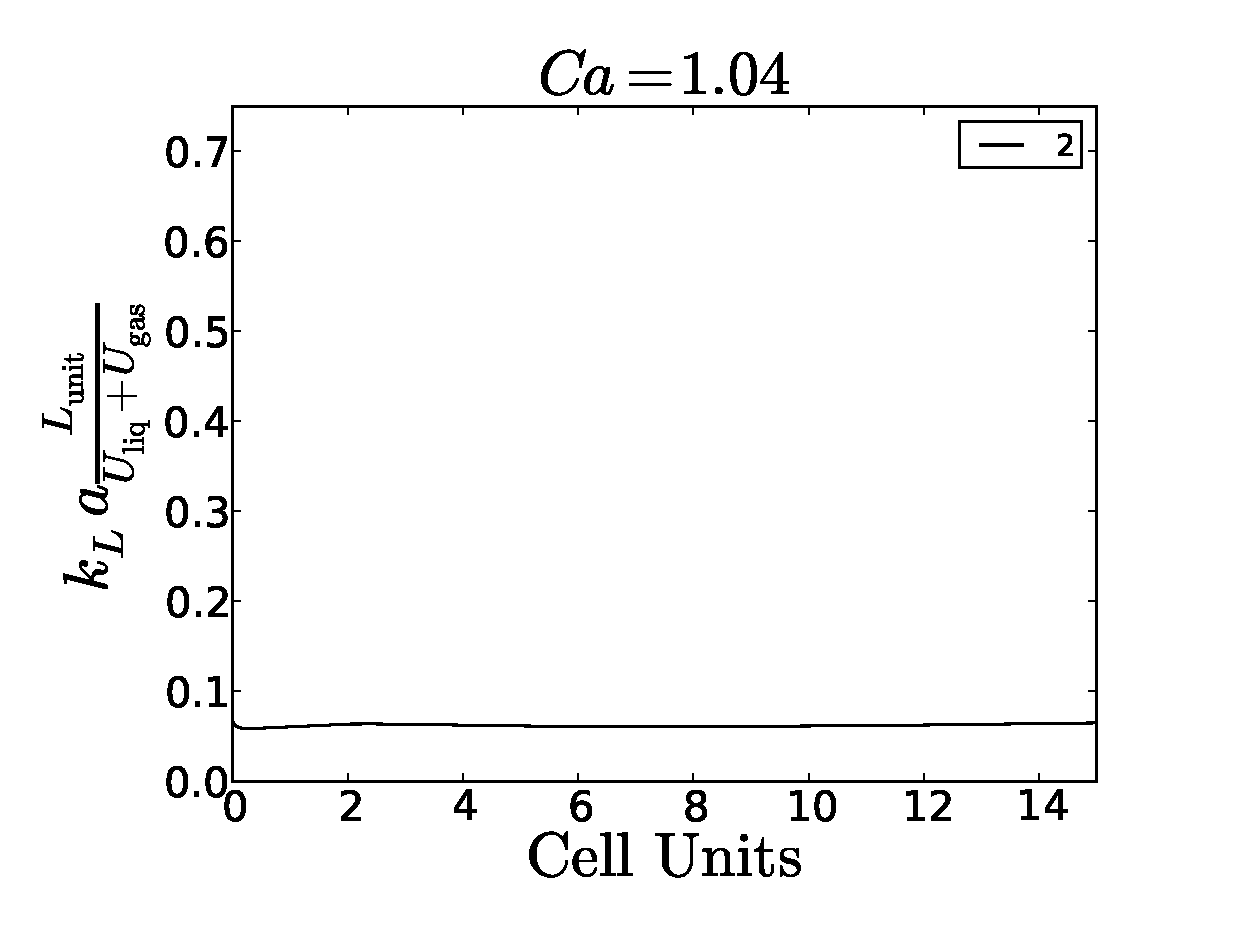
\includegraphics[width=0.5\textwidth]{vanbaten_aver_scale_ca14.eps}
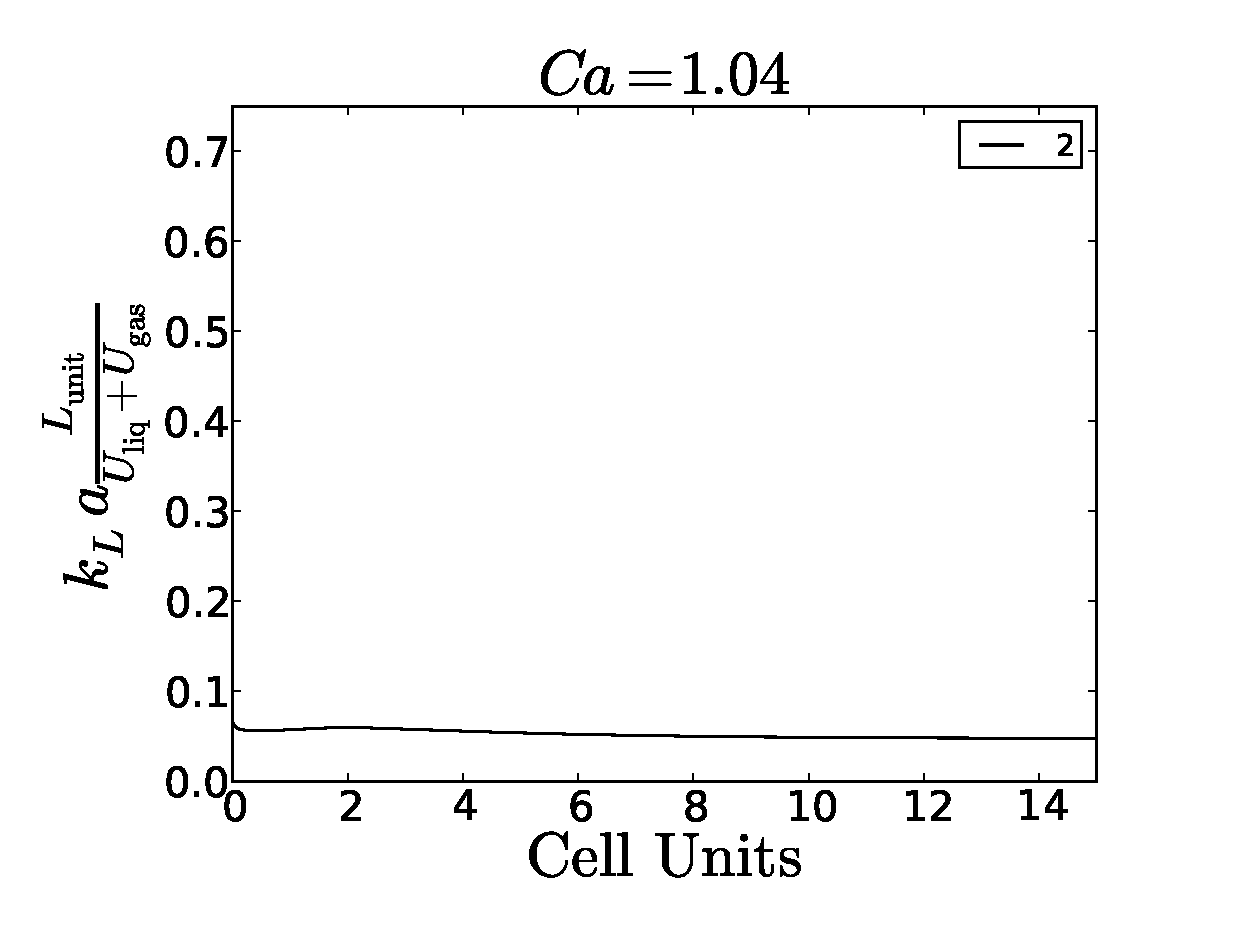
\includegraphics[width=0.5\textwidth]{vanbaten_full_scale_ca14.eps}\\
\caption{The \citet{vanbaten-circular} formulations for $Ca=0.097$ (top) and
$Ca=1.04$ (bottom) with the characteristic concentration being domain-averaged (left)
 and inlet/outlet flux-averaged (right). One can
see that the \citet{vanbaten-circular} formulation produces good results with the characteristic concentration being
the average concentration. Moreover, the values are closer to values obtained with many cell
simulations, see Fig. \ref{fig:moving:average:ca0097}, than in comparison with periodic boundary
simulations in Section \ref{main:results:periodic}. However, the characteristic concentration
being inlet/outlet flux-averaged does not produce consistent results.
\label{fig:vanbaten}}
\end{figure}

%\section{Open boundary conditions}
%\begin{figure}
%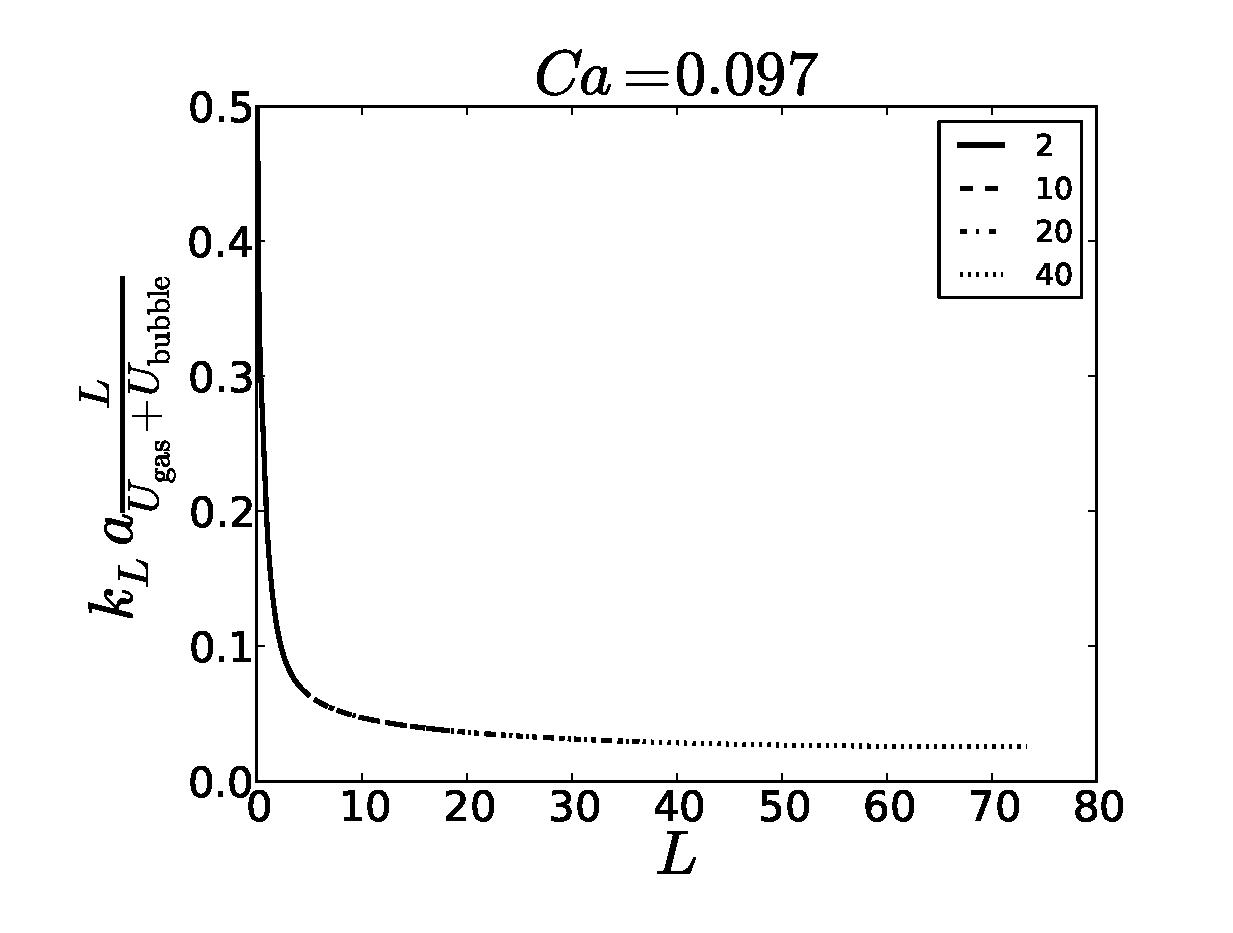
\includegraphics[width=0.5\textwidth]{Figures/jos_aver_conc_scale_ca0097.eps}
%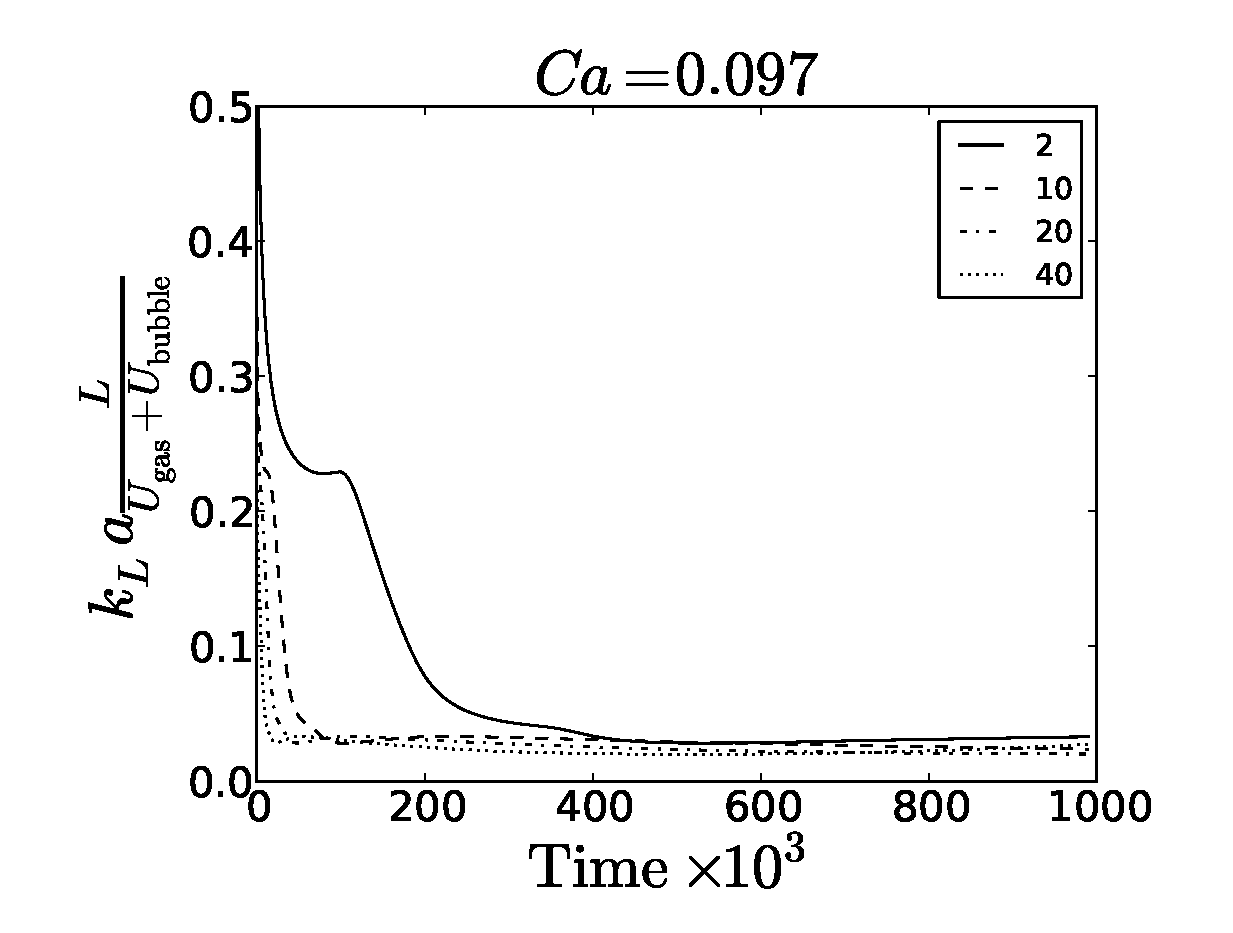
\includegraphics[width=0.5\textwidth]{Figures/jos_aver_moving_window_ca0097.eps}\\
%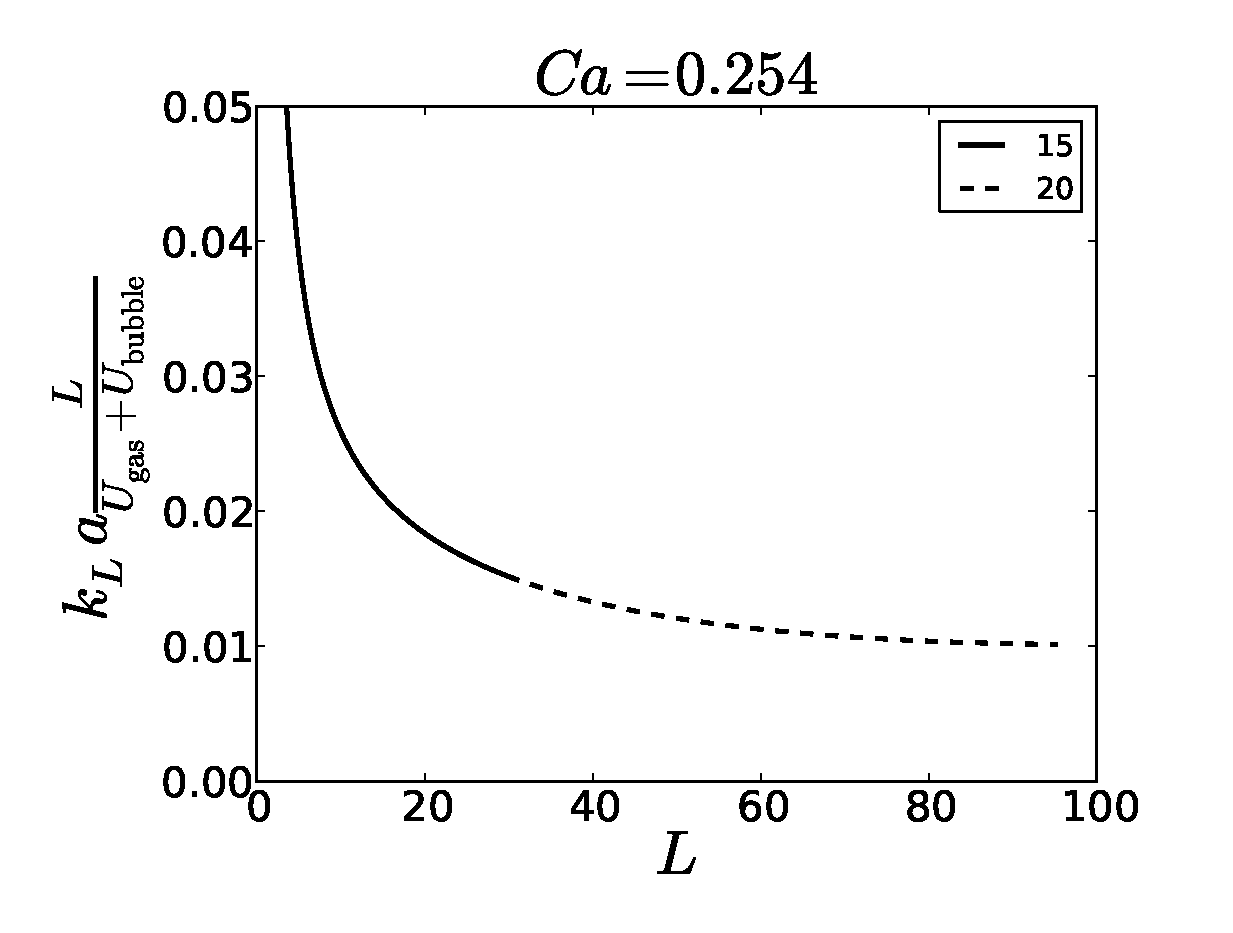
\includegraphics[width=0.5\textwidth]{Figures/jos_aver_conc_scale_ca0254.eps}
%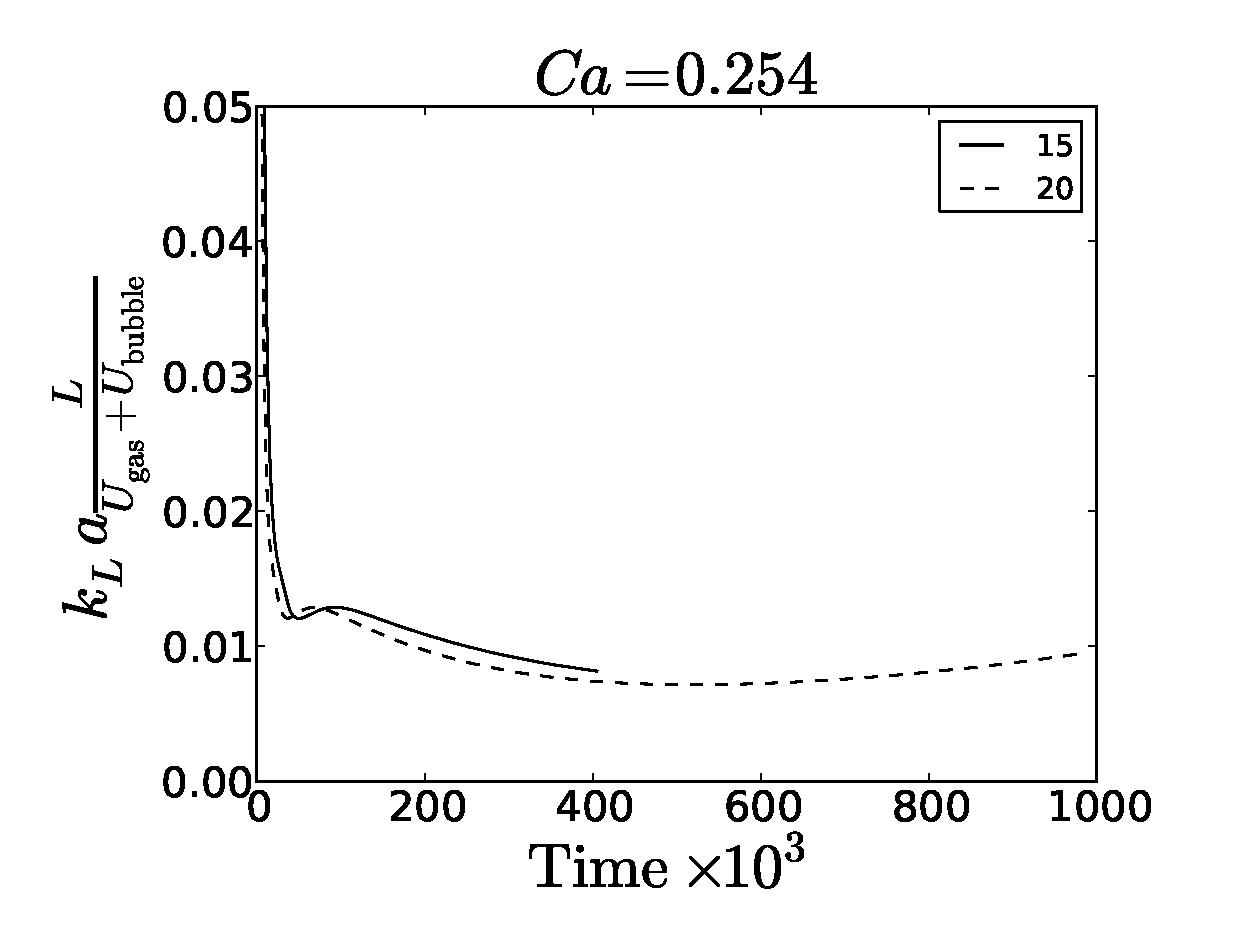
\includegraphics[width=0.5\textwidth]{Figures/jos_aver_moving_window_ca0254.eps}\\
%\caption{Open boundary conditions. \label{fig:open:boundary:jos}}
%\end{figure}
%\section{Symmetric boundary conditions}
%\begin{figure}
%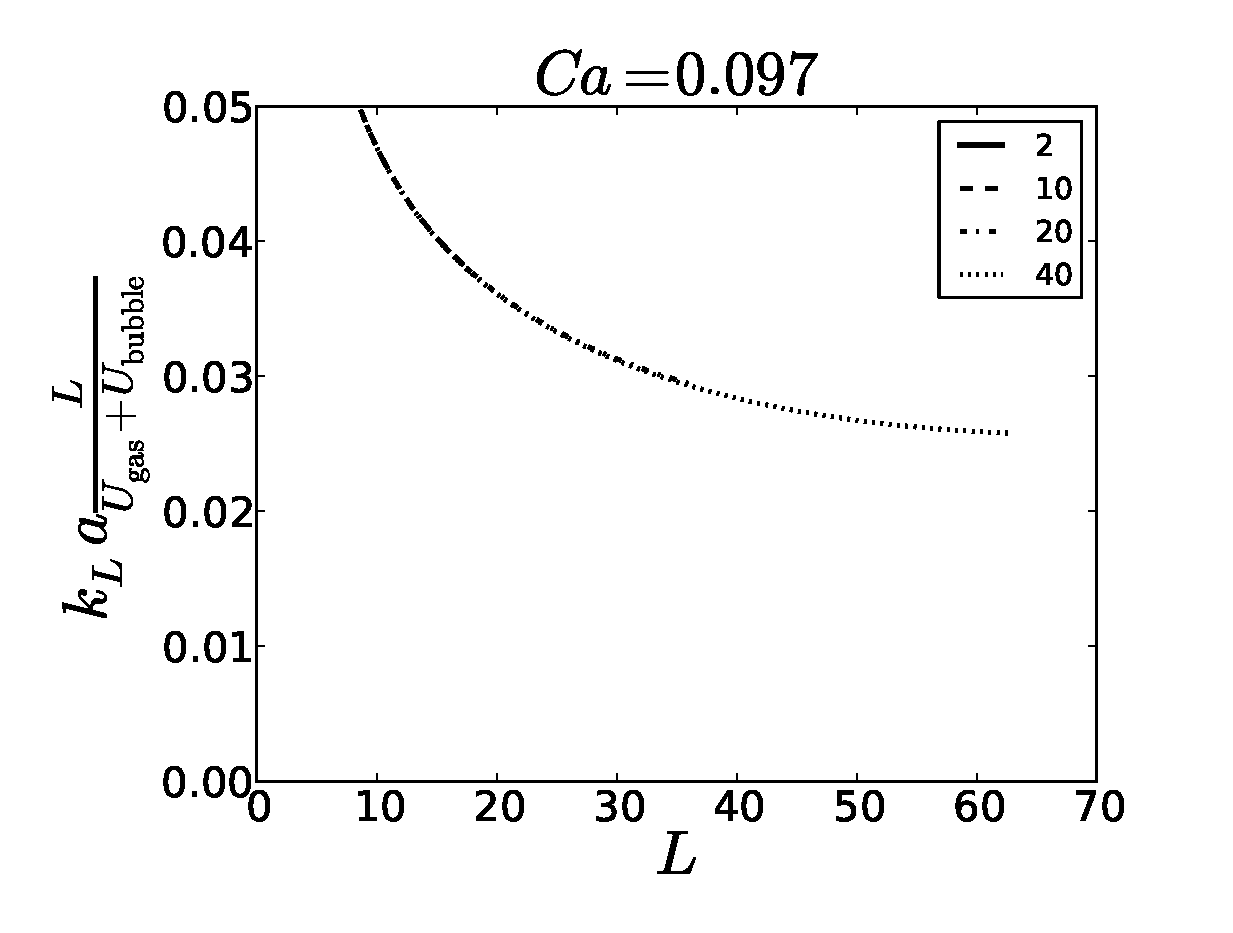
\includegraphics[width=0.5\textwidth]{Figures/sym_aver_conc_scale_ca0097.eps}
%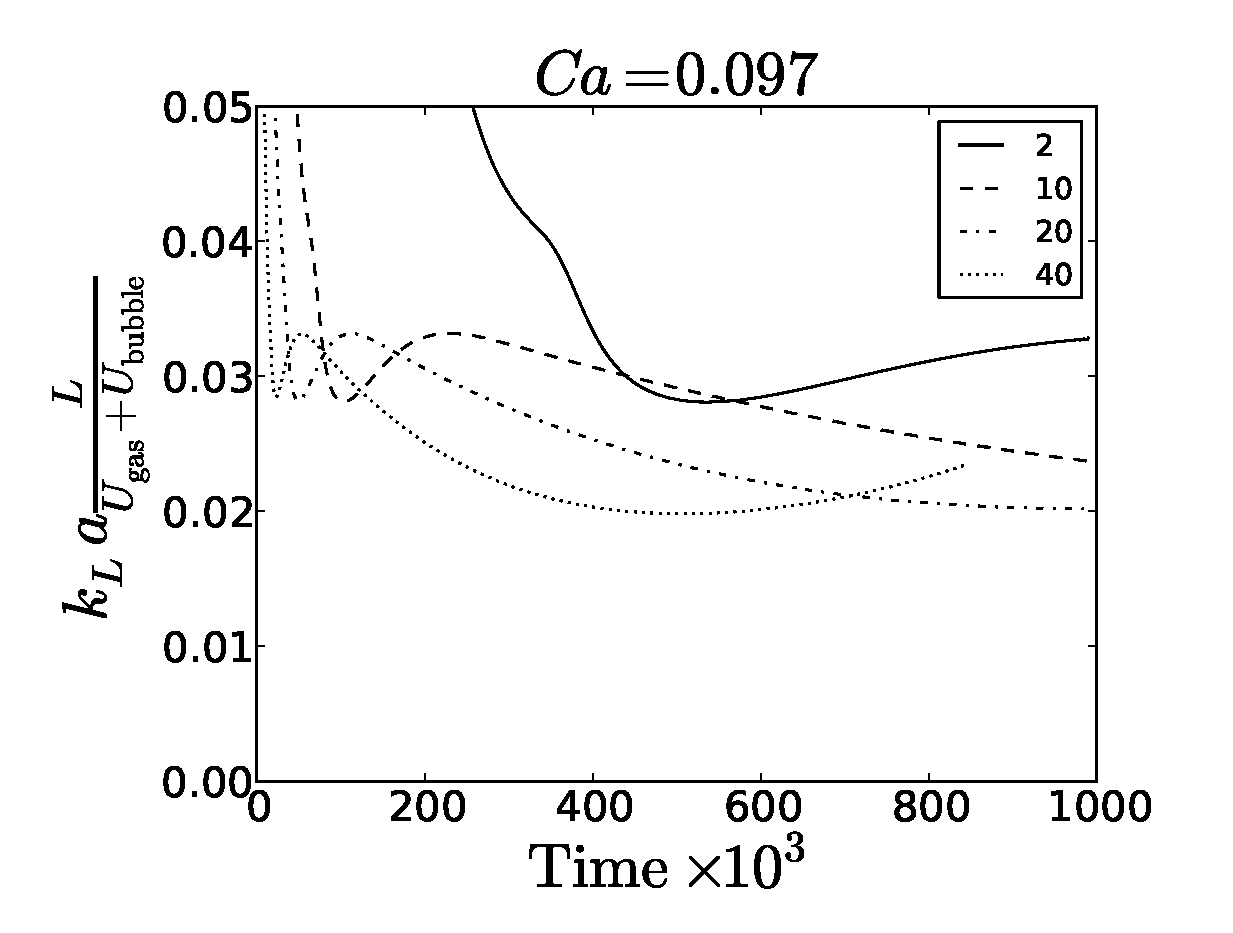
\includegraphics[width=0.5\textwidth]{Figures/sym_aver_moving_window_ca0097.eps}\\
%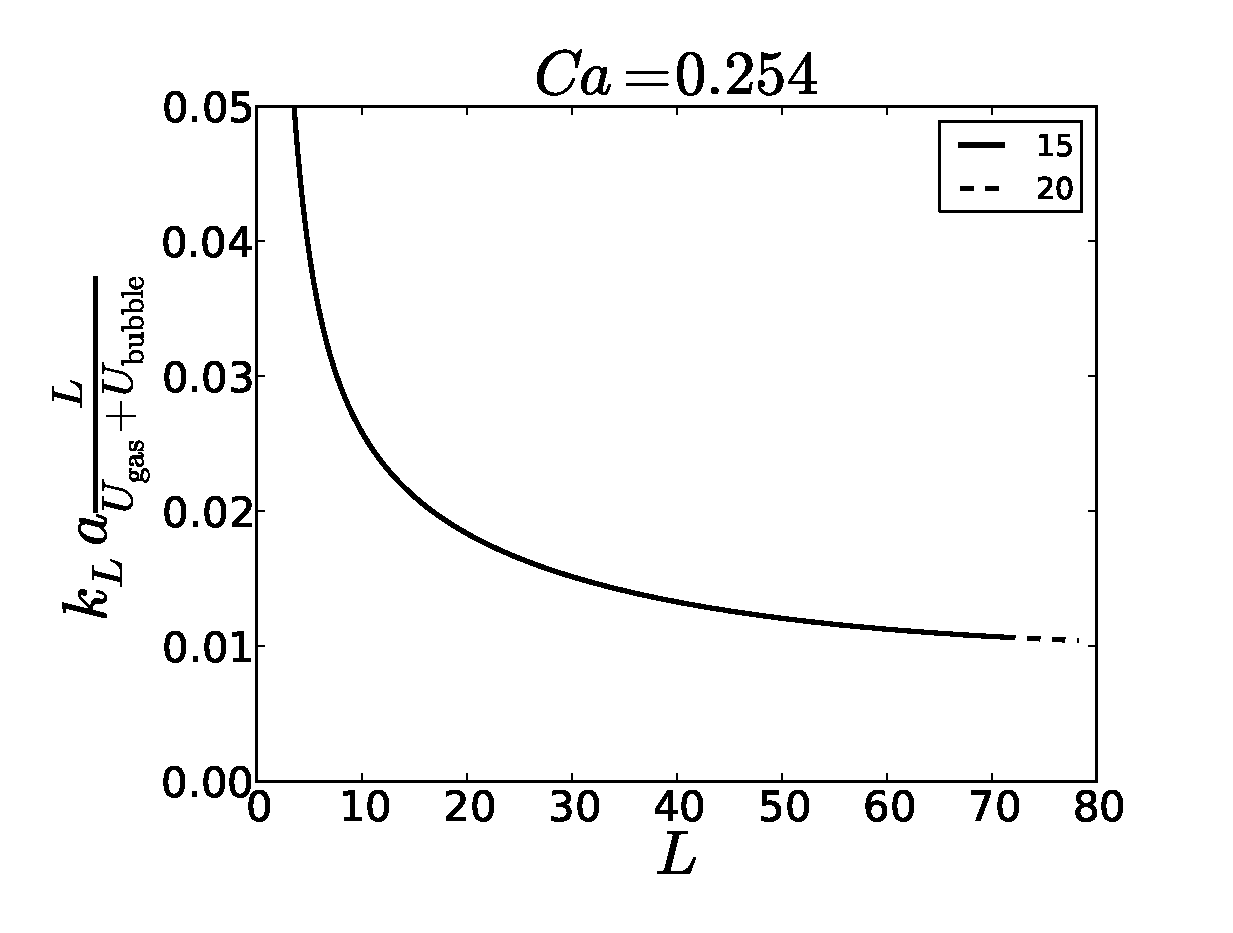
\includegraphics[width=0.5\textwidth]{Figures/sym_aver_conc_scale_ca0254.eps}
%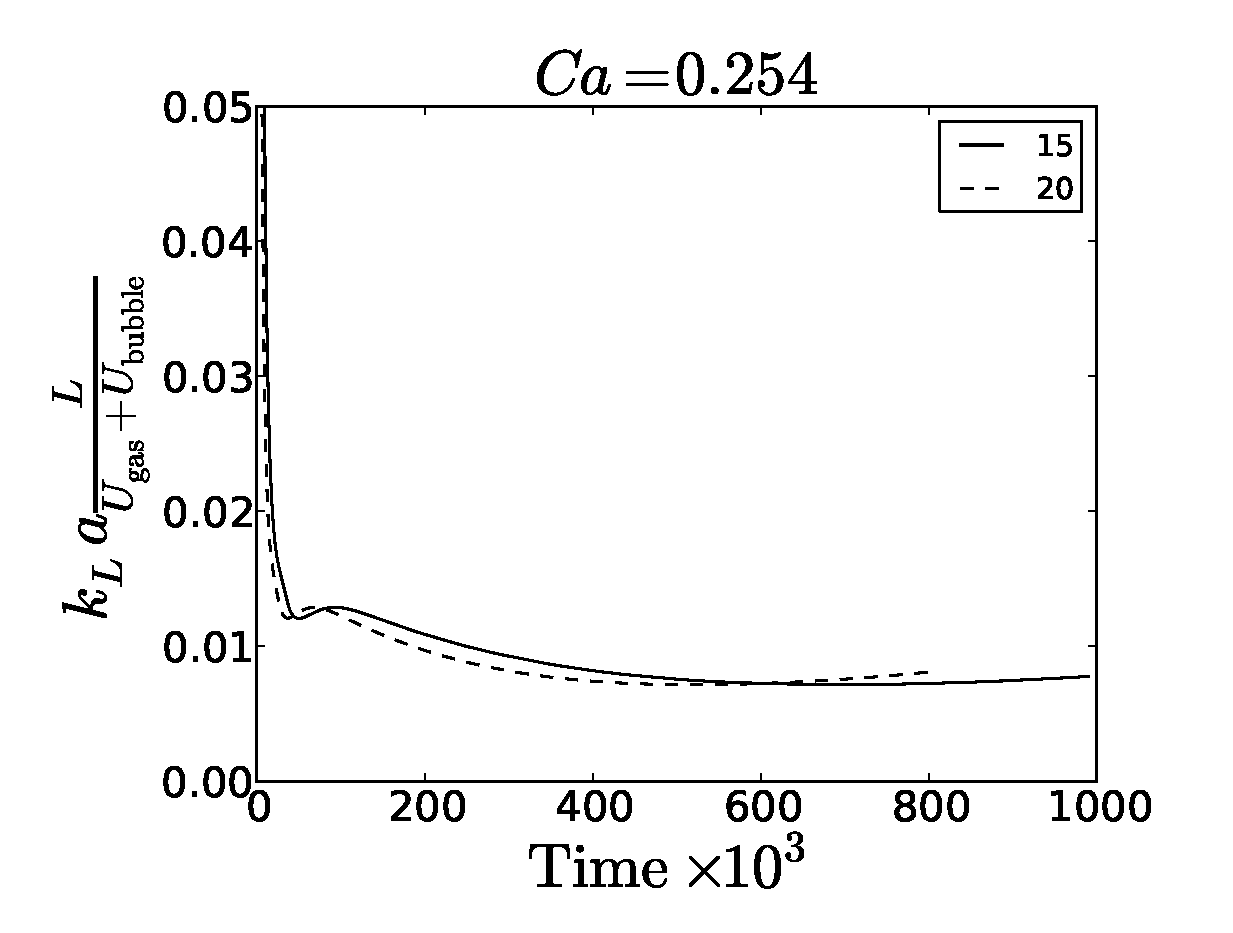
\includegraphics[width=0.5\textwidth]{Figures/sym_aver_moving_window_ca0254.eps}\\
%\caption{Symmetric boundary conditions. \label{fig:open:boundary:sym}}
%\end{figure}

\subsection{Simulations for several unit cells}
In order to achieve independence from the boundary conditions and a closer match with
the physical system being modelled, one can simulate several unit cells, corresponding
to a head of the bubble train.  If end effects are eliminated then the average
domain characteristic should change in time according to Eq.
\ref{theor:continuous:mass:transfer}. This eliminates the ambiguity inherent in choosing a definition
of the characteristic concentration, it becomes the same domain-averaged concentration
as the one measured in experiments.

This section studies the number of unit cells required for the volumetric
mass transfer coefficient to be independent of the influence of boundaries. We chose two
different
velocity patterns (see Fig. \ref{fig:streamlines:tweaked:velocity} for $Ca=0.097$ and $Ca=1.04$) to
perform the simulations. For $Ca=0.097$ we performed simulations with
$4$, $6$, $8$, $10$ cells, and for $Ca=1.040$ only with $4$, $6$, $8$ cells.
%The final run for 10 cells was skipped due to limited computational resources.
% TODO: how do we know that this holds true regardless of the Ca number?
We observed however that simulations with a domain length of $10$ unit cells produce the same results as those with $8$ unit cells.

We keep velocity in the range $0.05-0.1$ to avoid excessively long simulation times.
The number of steps for mass to pass through the whole domain can be approximated as $1.5 \frac{\lunit}{\ububble}$, which takes into account the bulk
velocity. If $\ububble$ is taken as $0.05$ then for
the domain size $\lunit=3000$ one can obtain the following number of iterations for the mass to
cross the unit cell $1.5 \frac{3000}{0.05}=90000$. Therefore, $10^{6}$ iterations are enough
for a system consisting of $10$ unit cells. For more accurate estimations of the number of time
steps depending on the Peclet number we refer to Section \ref{section:keeping:peclet}.

\subsection{$Ca=0.097$ results}
There are two characteristics we want to track in the simulations: the average
concentration in
the unit cell with time (see Eq. \ref{theor:continuous:mass:transfer}), and the accumulated mass
rate in the domain which takes into the account inlet/outlet fluxes (see Eq. \ref{main:main:main}). The former
resembles experiments: if one has a large enough number of unit cells, then the averaged domain
concentration should change in time according to Eq. \ref{theor:continuous:mass:transfer}: 
\beq
\label{moving:average}
\vol\frac{\lunit}{\ugas+\uliq}=\frac{\lunit}{\ububble (t_2
-t_1)}\ln\biggl(\frac{C^*-\langle C(t_1) \rangle}{C^*-\langle C(t_2)\rangle}\biggr)
\feq
The non-dimensional volumetric mass transfer coefficient calculated based on Eq.
\ref{moving:average} (domain-averaged concentration change in time) is
represented in Fig. \ref{fig:moving:average:ca0097} for different unit cells. One can see that mass transfer coefficient values are the same as the mass flux
concentration based on the \citeauthor{vanbaten-circular} formulation with the characteristic
concentration being the domain-averaged concentration (see Section
\ref{results:vanbaten}). This demonstrates two things:  the domain-averaged
concentration is the only choice for the characteristic concentration, and
periodic boundary conditions for one unit cell produce good results.

%The
%latter is the main equation that can help to obtain the volumetric mass transfer coefficient from
%mass transfer simulations with any bounary conditions (periodic boundary conditions, open
%boundaries). 
In comparison with periodic boundary conditions Eq.~\ref{main:main:main} allows
to calculate the mass transfer coefficient differently. Eq.
\ref{main:main:main}  can be rewritten as: \beq
\label{main:main:main:thorough}
\begin{aligned}
\volnondim=\frac{\lunit}{\ugas+\ububble} \frac{V \frac{\langle C(t_2)\rangle - \langle C(t_1)
\rangle}{t_2-t_1}}{}\\
\frac{-\int{\coutlet(\lunit,y,t^*) u(\lunit,y) \mathrm{d} y}+\int{\cinlet(0,y,t^*)
u(0,y)\mathrm{d} y}}{V (\cstar - \langle C(t^*) \rangle)},
\end{aligned}
\feq
where $t^*$ is the mean between $t_1$ and $t_2$.
%TODO: what is a medium time?  is it just the mean of the two times?


%The
%argument behind this characteristic is that if the following situation is fulfilled: the continuity
%equation is satisfied then the concentration along the coordinate changes according to Eq.
%\ref{main:mass:transfer:expression}:
%\beq
%C(x)= \cstar \Bigl(1-\exp\bigl(-\vol \frac{x}{\uliq+\ugas} \bigr)\Bigr)
%\feq
%After the transition to the reference frame moving with the velocity $\ububble$, one will have the
%same continuous picture but the concentration dependency will change since velocity is changed as
%well:
%\beq
%C(x)= \cstar \Bigl(1-\exp\bigl(-\vol \frac{x}{\uliq+\ugas-\ububble} \bigr)\Bigr),
%\feq
%Thus, the volumetric mass transfer coefficient for two concentrations which are located at the
%distance $\lunit$ can be found as:
%\beqal
%&\vol \frac{\lunit}{\uliq+\ugas-\ububble}=\ln\Bigl(\frac{\cstar-C_1}{\cstar-C_2}\Bigr)\\
%&\vol
%\frac{\lunit}{\uliq+\ugas}=\frac{\uliq+\ugas-\ububble}{\uliq+\ugas}\ln\Bigl(\frac{\cstar-C_1}{
%\cstar-C_2}\Bigr)
%\feqal
%Parameters $\frac{\uliq+\ugas-\ububble}{\uliq+\ugas}$ were calculated and for representative
%Capillary numbers equal to $0.11,0.04,-0.02,-0.06,-0.10$.
%In the case of present simulations the situation is different as the reference frame is moving with
%the bubble. Thus, the correlation between adjacent cells as follows:
%\beqal
%\label{volumetric:between:adjacent:cells}
%&C_1=C(x)=C^* \Bigl(1-e^{-\vol \frac{x}{\ugas+\uliq-\ububble}}\Bigr)\\
%&C_2=C(x+L)=C^* \Bigl(1-e^{-\vol \frac{x+L}{\ugas+\uliq-\ububble}}\Bigr)\\
%&k_L\frac{L}{\ugas+\uliq-\ububble}=\frac{C^*-C_1}{C^{*}-C_2}\\
%&k_L\frac{L}{U}=\frac{C^*-C_1}{C^*-C_2},
%\feqal
%where $U=\ugas+\uliq-\ububble$. We will see later that this characteristic is really important to
%see whether the liquid slug is mixed. 
Fig.~\ref{fig:unit:6} shows average concentrations in different units and $\volnondim$ based on
Eq.~\ref{main:main:main:thorough} calculated for each unit for velocity
scale $10$ and  $6$ unit cells (all velocity scales produce the same results). It shows that the
volumetric mass transfer coefficient is consistent for internal segments, i.e.
unit cells numbers $2-4$.  The results for the volumetric mass transfer
coefficient calculated by Eq. \ref{main:main:main} for multiple unit cells are
close (less than $10\%$ deviation) to results for periodic boundary conditions in Section
\ref{main:results:periodic} . 
%However, they are even closer to results calculated by approach of \citeauthor{vanbaten-circular} with the domain averaged characteristic concentration. 
The same dependencies
can be found for
$8$ and $10$ unit cells simulations but we do not present them here. We also do not present $4$
units cells simulation results which are highly influenced by entrance and exit effects.

The calculation of the  volumetric mass transfer coefficient is more difficult
using Eq. \ref{main:main:main:thorough}. However, it will be shown below that
this equation can be significantly simplified in case of larger capillary
numbers ($Ca>0.7$).

\begin{figure}[htb!]
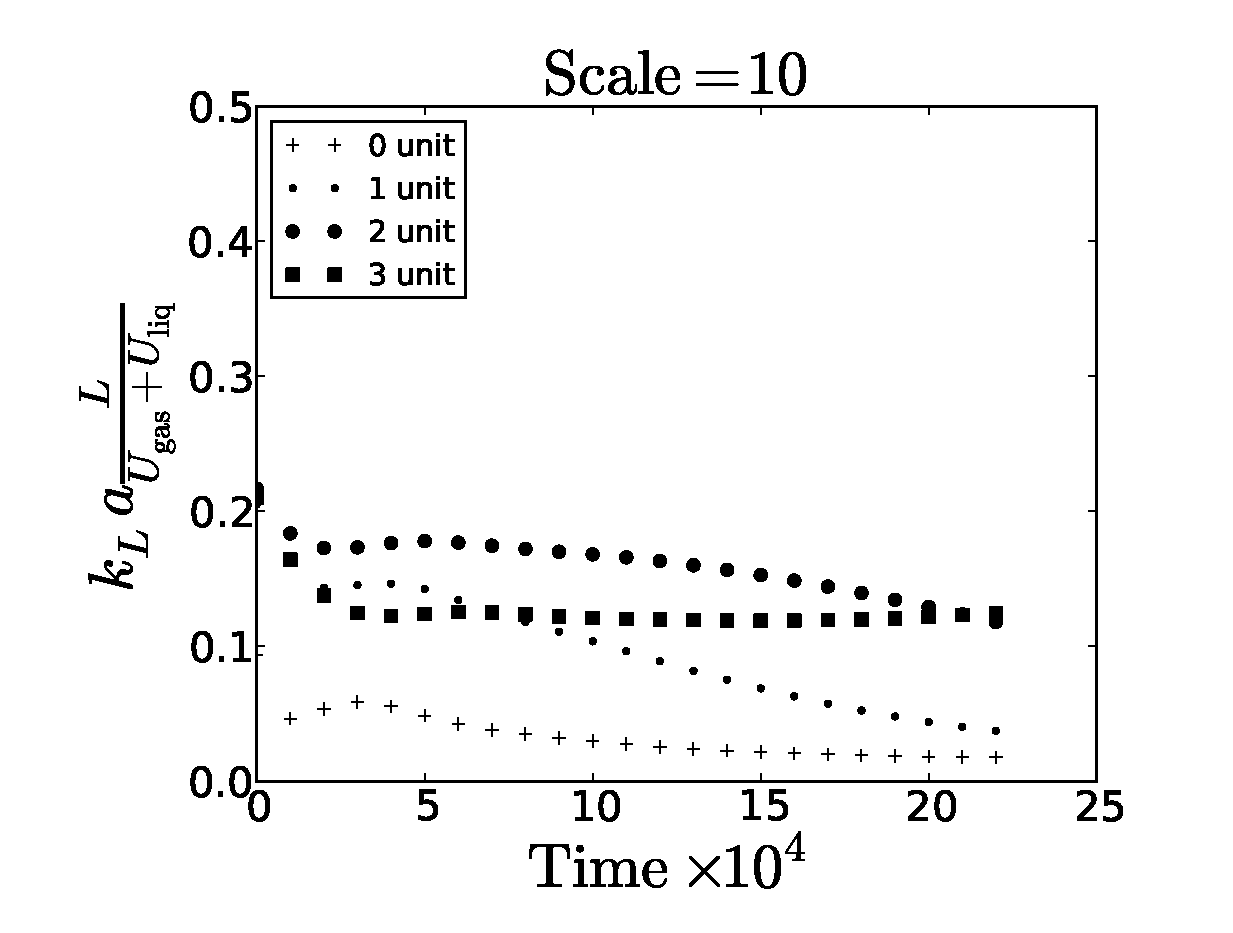
\includegraphics[width=0.5\textwidth]{aver_moving_window4scale10.eps}
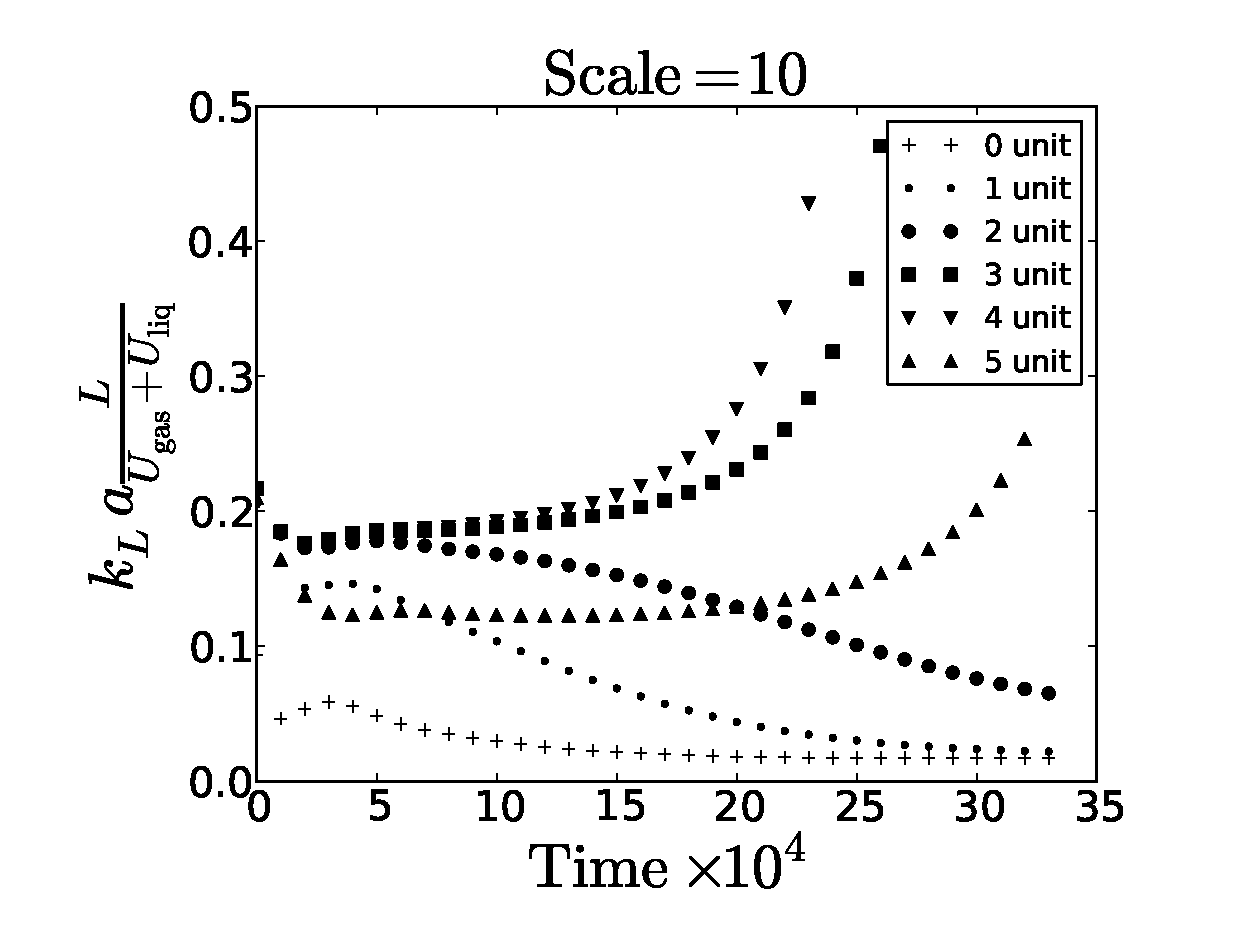
\includegraphics[width=0.5\textwidth]{aver_moving_window6scale10.eps}\\
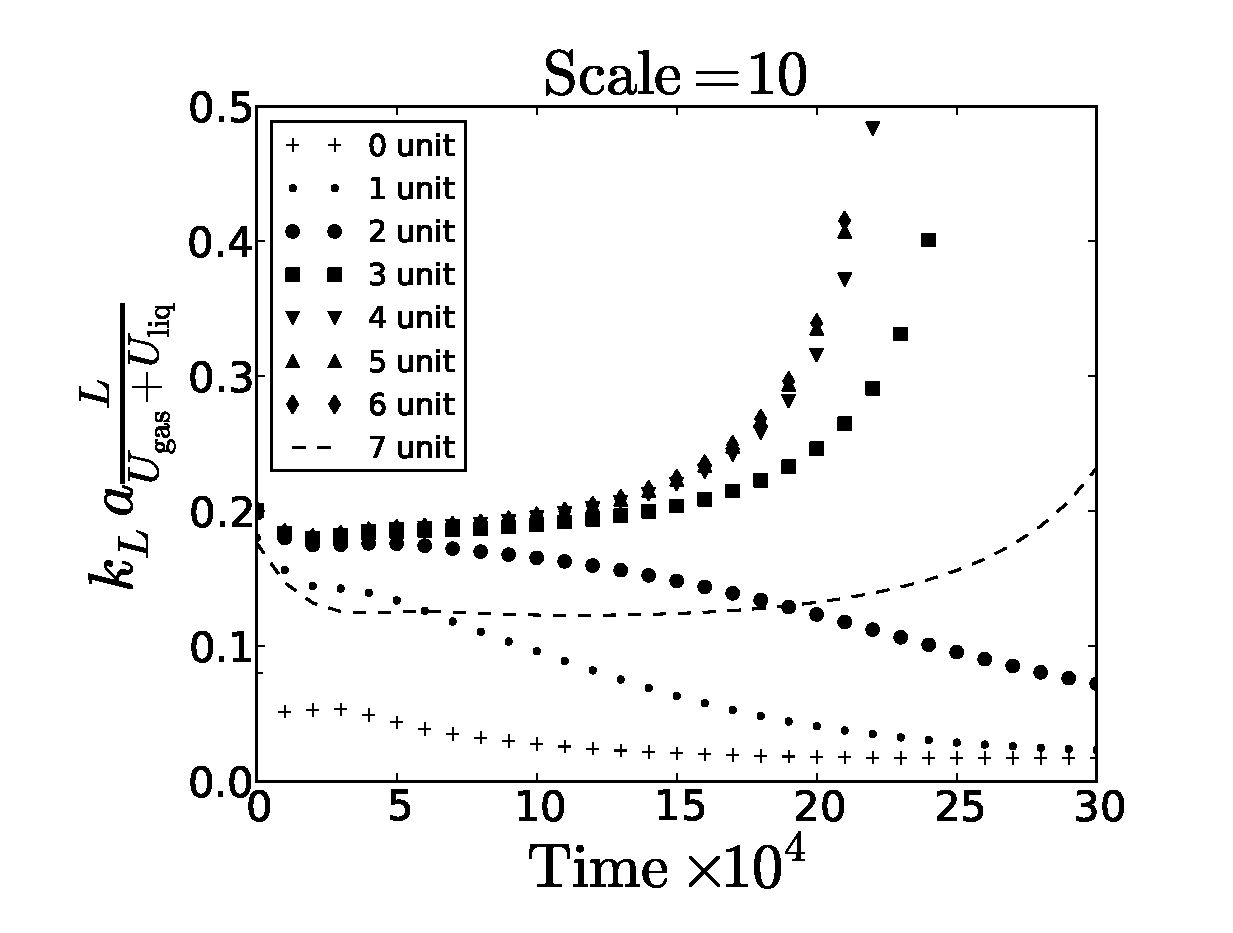
\includegraphics[width=0.5\textwidth]{aver_moving_window8scale10.eps}
\caption{The non-dimensional volumetric mass transfer coefficient defined in Eq.
\ref{moving:average} for $4$ (top left), $6$ (top right), $8$ unit cells (bottom). Only scale
$10$ is presented since all other simulations produce the same results. One can see that $4$ unit
cells is not enough to avoid the influence of boundaries. However, the results for $6$ and $8$
unit cells are consistent and show that beginning from third unit cell the results and ending with
the penultimate cell results are consistent with periodic boundary simulations and
\citet{vanbaten-circular} formulations.
\label{fig:moving:average:ca0097}}
\end{figure}
\begin{figure}[htb!]
%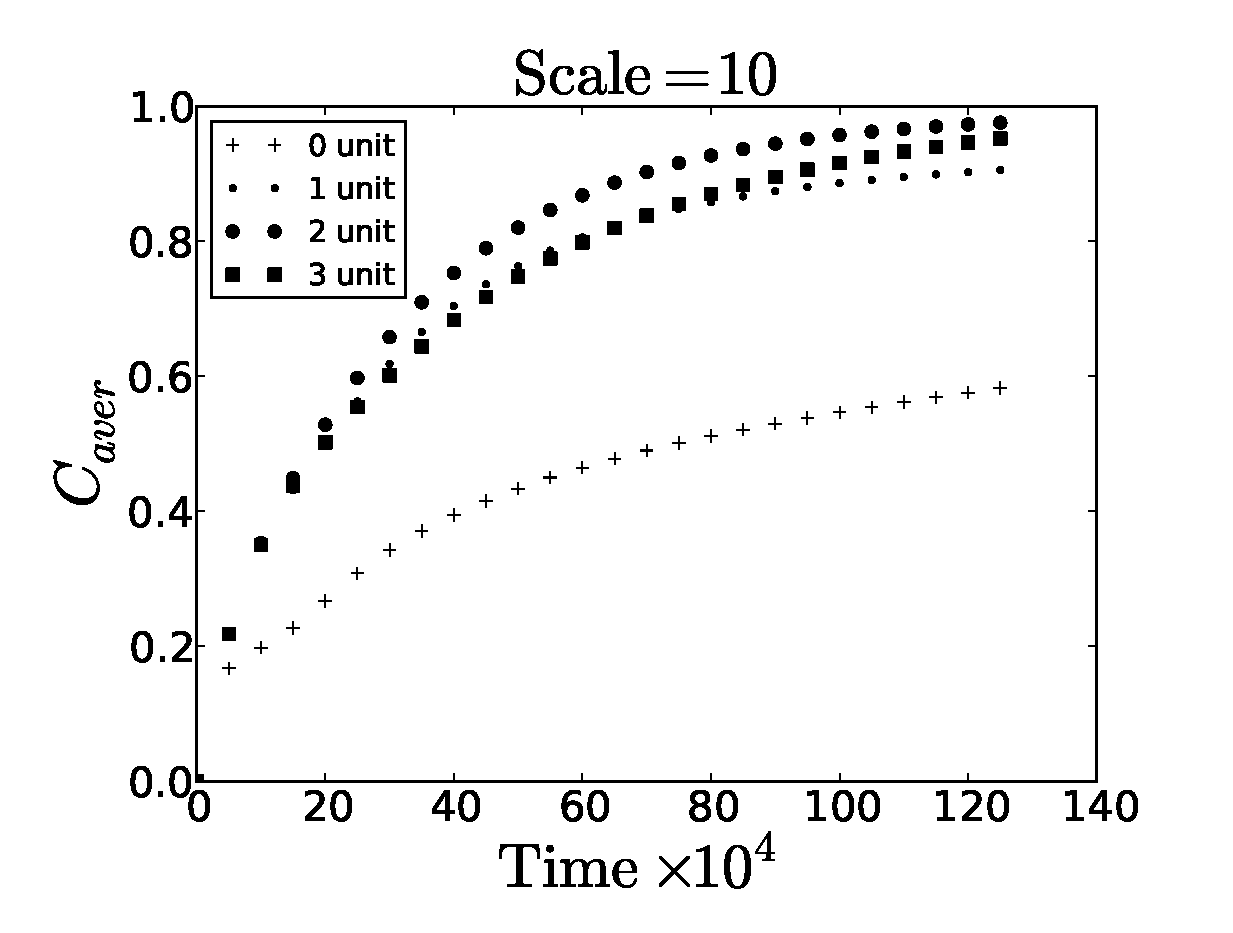
\includegraphics[width=0.5\textwidth]{Figures/aver_units4scale10.eps}\hfill
%\includegraphics[width=0.5\textwidth]{Figures/coeff_units4scale10.eps}\\
%\includegraphics[width=0.5\textwidth]{Figures/aver_units4scale15.eps}\hfill
%\includegraphics[width=0.5\textwidth]{Figures/coeff_units4scale15.eps}\\
\includegraphics[width=0.5\textwidth]{aver_units6scale10.eps}\hfill
\includegraphics[width=0.5\textwidth]{right_def_6scale10.eps}\\
%\includegraphics[width=0.5\textwidth]{Figures/coeff_units4scale20.eps}\\
\caption{Average concentrations (left) and volumetric coefficients (right) for $6$ unit cells. The
volumetric
mass transfer coefficient is calculated based on Eq. \ref{main:main:main:thorough} and accounts for inlet
and outlet fluxes. \label{fig:unit:6}}
\end{figure}

\subsection{$Ca=1.040$ results}
The same correlations were examined for a different velocity pattern at $Ca=1.040$. %, initial
%velocity $\ububble=0.055$, initial diffusion $D=0.0008375$. If only velocity scaling is
%performed then a few unit cells simulations for
%this capillary number  are unstable. 
The original Peclet number we started with is $Pe=14041$ (Table \ref{table:scaling:peclet}).
To improve stability we changed the original Peclet number by increasing
diffusion to $Pe=2644$. The results with respect to the number of unit cells are the same as for $Ca=0.097$:
at least $6$ unit cells are required to avoid the influence of inlet/outlet effects. Thus,
only $6$ unit cells results are presented in Fig. \ref{fig:6:units:ca1040} which shows the
average concentration for each unit cell. One can see that the average volume concentration for each unit cell converges to
a constant value. Thus, all the
mass generated by the bubble is transferred through the boundaries. This indicates that the
liquid slug is unmixed since no concentration travels back to inlet with the vortex and increases the average concentration in each unit cell. Note that the periodic boundary conditions cannot show whether the
liquid slug is mixed or not due to the fact that the averaged domain concentration always increases in time. 
Thus, the volumetric mass transfer coefficient $\volnondim$ can be calculated according to the
definition, Eq. \ref{main:main:main}:
\beq
\label{inlet:outlet:spatial:location}
\vol =
\frac{\dot{m}-\int{\coutlet(y)u(\lunit,y)\mathrm{d}y}+\int{\cinlet(y)u(\lunit,y)\mathrm{d}y}}{V
(\cstar - \langle C(t) \rangle},
\feq 
where $V$ is the unit cell volume. There is no accumulated mass in the domain, so $\dot{m}=0$. Like periodic boundary
conditions, this case is another extreme limit of Eq. \ref{main:main:main}. Note that to calculate
the volumetric mass transfer coefficient one needs only the spatial information and does not
require the knowledge of how the averaged concentration changes in time, which significantly
lowers storage requirements for the simulations with $Ca>0.7$ where there is no vortex in the
liquid slug. 

Fig. \ref{fig:periodic:ca1040}
(bottom) shows the volumetric mass transfer coefficient based on spatial calculations of
inlet/outlet concentrations. One can see that the volumetric mass transfer coefficient is close to
the calculated volumetric mass transfer coefficient using the time averaged approach and periodic
boundaries one unit cell simulations (presented in the same figure for comparison).
\begin{figure}[htb!]
\begin{center}
\includegraphics[width=0.5\textwidth]{aver_units6scaleu2scaled5.eps}
\end{center}
%\includegraphics[width=0.5\textwidth]{Figures/novortex6scaleu2scaled5.eps}\\
\caption{Results for $6$ unit cells. The Peclet number equals to $Pe=2644$.
One can see that average concentrations reach certain value and stay constant.
%That means whatever was
%generated by medium is transferred through the outlet
%boundary. This indicates that the tracer in the slug is not
%mixed and t
Thus, the volumetric mass transfer coefficient, $\volnondim$, can be
calculated using the spatial approach, see Fig.
\ref{fig:periodic:ca1040}.
\label{fig:6:units:ca1040}}
\end{figure}
%The volumetric mass transfer coefficient with periodic boundary simulations for $Pe=2644$ (velocity
%scale $2$, diffusion scale $10$) and time dependent, Eq. \ref{theor:continuous:mass:transfer},
%average volumetric mass transfer coefficient are presented in Fig. \ref{fig:periodic:ca1040}. 
Note
that results for approaches which incorporate the volume-averaged characteristic concentration either for one cell or a few unit cells coincide. Therefore, for certain hydrodynamic patterns ($Ca>0.7$), one can
easily convert time domain to spatial domain calculations using simulations of several unit cells.
\begin{figure}
\includegraphics[width=0.5\textwidth]{volume_ca_104_scaleu2scaled5.eps}
\includegraphics[width=0.5\textwidth]{aver_moving_window6scaleu2scaled5.eps}\\
\includegraphics[width=0.5\textwidth]{flux_moving_window6scaleu2scaled5.eps}\\
\caption{The periodic (top left, $1$ unit cell, Eq. \ref{theor:continuous:mass:transfer}), unit
cells domain-averaged concentrations as a function of time (top right, $6$ unit cells, Eq.
\ref{theor:continuous:mass:transfer}), and spatial location
(bottom, $6$ unit cells, Eq. \ref{inlet:outlet:spatial:location}) calculated  volumetric mass
transfer
coefficients. One can see that they all coincide. However, the calculations based on periodic boundary conditions
produce a slightly overestimated volumetric mass transfer
coefficient. One can as well see that the domain-averaged concentration simulations (top right)
reach the steady volumetric concentration fast and start decaying after that. It is not convenient
to use them in practical cases for unmixed slug, i.e. $Ca>0.7$. \label{fig:periodic:ca1040}}
\end{figure}

\subsection{Comparison of experimental and analytical correlations}
While the goal of this paper is not to compare simulation results with the experimental measurements, 
we felt that a short note about such comparison will be beneficial.
Unfortunately, to the authors' knowledge, there are no reported experimental results measuring the mass flux for
  bubbles flowing between parallel plates. However, an interesting
correlation for the mass transfer volumetric coefficient was presented by
\citet{yue-mass} for three-dimensional microchannel geometries:
\beqal
&\vol=\frac{2}{d_h}\Bigl(\frac{D \ububble}{\lbubble+\lslug}\Bigr)^{0.5}
\Bigl(\frac{\lbubble}{\lbubble+\lslug}\Bigr)^{0.3}\\
&\vol \frac{\lunit}{\ugas+\uliq}=2\frac{\lunit}{d_h} \Bigl(\frac{D 
}{\lunit (\ububble+\ugas)} \frac{\ububble}{\ugas+\uliq}\Bigr)^{0.5}
\Bigl(\frac{\lbubble}{\lbubble+\lslug}\Bigr)^{0.3} \propto Pe^{-\frac{1}{2}}\\
\feqal
One can see that  the volumetric mass transfer correlation should be approximately proportional to
$Pe^{-0.5}$.  One can also use analytical estimates of the volumetric mass transfer
coefficient calculated using the Higbie penetration theory \cite{higbie}. One can derive the analytical expression for the mass transfer for bubble train flow between parallel plates by following the works
\cite{irandoust,vanbaten-circular}:
\beq
\label{vanbaten:analytical:expresssion}
\begin{aligned}
\volnondim=&\frac{\lunit}{\ugas+\uliq}\Bigl(4 \sqrt{D \ububble}{\pi}
\frac{\sqrt{\lbubble-H (1-2\delta)}}{\lunit H}\\
&+2 \sqrt{2} \sqrt{D \ububble} \frac{\sqrt{H
(1-2\delta)}}{\lunit H}\Bigr),
\end{aligned}
\feq
where $H$ is the channel height, and $\delta$ is the non-dimensional film thickness (in channel heights).

Fig. \ref{fig:volume:mass:coefficient} shows a comparison between the correlation by
\citet{yue-mass}, the analytical expression, Eq. \ref{vanbaten:analytical:expresssion}, and the current
simulation results presented in Table
\ref{table:steady:state:average}. The coefficients are close to each other, especially given that
the correlation by \citet{yue-mass} is for three-dimensional cases. The fitting procedure for this work results showed
that the power of
the Peclet number dependence  is $-0.50038$ which is close to the theoretical value $-0.5$.  The fitting curve is $7.745 Pe^{-0.50038}$.
\begin{figure}[htb!]
\includegraphics[width=\textwidth]{correlations_comparison.eps}
\caption{Comparison between the correlation by \citet{yue-mass}, the analytical correlation derived by following the work
\cite{irandoust} and the mass transfer coefficient based
on periodic boundary conditions. The fitting curve ($7.745 Pe^{-0.50038}$) is proportional to $Pe^{-0.5}$ which corresponds
to all correlations. One can as well see that the deviation from the analytical expression becomes
larger with the increasing Peclet number, which happens because the analytical expression does
 not account for the velocity pattern and the bubble shape change.\label{fig:volume:mass:coefficient}}
\end{figure}

\section{Summary}
This work examines a way to calculate the volumetric mass transfer coefficient of Taylor/Batchelor bubble train flow in the framework of
the lattice Boltzmann method. Overall, the easiest recipe is to perform simulations 
with periodic boundary conditions
and calculate the volumetric mass transfer coefficient based on the
domain-averaged concentration through any formulation (\citeauthor{vanbaten-circular}, periodic boundary conditions, simulations of several unit cells) as they produce consistent results. The best accuracy
is achieved with formulations based on the mass difference or on the averaged domain concentrations
taken in different times, Eq. \ref{theor:continuous:mass:transfer}. Eq.
\ref{theor:average:concentration:time} gives a slightly overestimated volumetric mass transfer
coefficients (less than $10\%$). The original formulation of
\citet{vanbaten-circular} is inconsistent if one takes the inlet/outlet flux-averaged concentration
to be the characteristic concentration. Simulations of several unit cells are harder to perform, but they
indicate how well the liquid slug is mixed.  For velocity patterns related to $Ca\geq
0.7$ simulations with a few unit cells allow to calculate the volumetric mass transfer
coefficient based on the spatial location only, without requiring the time snapshots of domain concentration values used in all other
approaches. Finally, a sample of results was
compared with the experimental correlation of \citet{yue-mass} and shown to be consistent. 

\section{Acknowledgements}
M.J. acknowledges a scholarship from the TWING project co-financed by the European Social Fund. A.K. wants to thank Schlumberger for their financial support.

\appendix
%\section{Analytical solution for parabolic profile with zero velocity gradient at $0$}
%\label{appendix:zero:gradient}
%The problem is defined in terms of PDE as follows: 
%\beq
%\label{diffusion:zero:gradient:start}
%\begin{aligned}
%&\frac{\partial C}{\partial x} U(y)=D\frac{\partial^2 C}{\partial y^2}\\
%&C(0,y)=C_0,\, C(x,0)=\cstar,\, \frac{\partial C}{\partial y }(x,\delta)=0\\
%&U(y)=U_0 \Bigl(\frac{y}{\delta}\Bigr)^2
%\end{aligned}
%\feq
%The non-dimensional parameters are introduced:
%\beq
%\begin{aligned}
%&\frac{\partial C}{\partial \frac{x}{\delta}} \frac{U_0}{\delta}
%\Bigl(\frac{y}{\delta}\Bigr)^2=\frac{D}{\delta^2}\frac{\partial^2 C}{\partial
%\frac{y^2}{\delta^2}}\\
%&C(0,y)=C_0,\, C(x,0)=\cstar,\, \frac{\partial C}{\partial y }(x,\delta)=0\\
%\end{aligned}
%\feq
%After a change of variables:
%\beq
%\begin{aligned}
%&\zeta=\frac{x}{\delta} \frac{D}{U_0 \delta}=\frac{1}{Pe}\frac{x}{\delta}\\
%&\xi=\frac{y}{\delta},
%\end{aligned}
%\feq 
%Eq. \ref{diffusion:zero:gradient:start} with boundary conditions becomes as follows:
%\beq
%\label{diffusion:zero:gradient:middle}
%\begin{aligned}
%&\frac{\partial C}{\partial \zeta}\xi^2=\frac{\partial^2 C}{\partial \xi^2}\\
%&C(0,\xi)=C_0\\
%&C(\zeta,0)=\cstar\\
%&\frac{\partial C}{\partial \xi}(\zeta,1)=0\\
%\end{aligned}
%\feq 
%Still Eq. \ref{diffusion:zero:gradient:middle} cannot be solved with the separation of variables as it requires homogenous
%boundary conditions. Thus, let us introduce the new variable, $\Theta=C-\cstar$, which makes the system have homogenous boundary conditions:
%\beq
%\begin{aligned}
%&\frac{\partial \Theta}{\partial \zeta}=\frac{1}{\xi^2}\frac{\partial^2 \Theta}{\partial \xi^2}\\
%&\Theta(0,\xi)=C_0-\cstar \\
%&\Theta(\zeta,0)=0,\, \partial_{\xi}\Theta(\zeta,1)=0\\
%\end{aligned}
%\feq 
%This equation can be solved by separation of variables if the solutions are assumed to factorize as
%$\Theta(\zeta,\xi)=X(\zeta)Y(\xi)$:
%\beq
%\begin{aligned}
%&\frac{\mathrm{d} X(\zeta)}{\mathrm{d} \zeta}Y(\xi)=\frac{X(\zeta)}{\xi^2}\frac{\mathrm{d^2}
%Y(\xi)}{\mathrm{d}\xi^2}\\
%&\frac{1}{X(\zeta)}\frac{\mathrm{d} X(\zeta)}{\mathrm{d} \zeta}=\frac{1}{\xi^{2} Y(\xi)}
%\frac{\mathrm{d^2} Y(\xi)}{\mathrm{d}\xi^2}
%\end{aligned}
%\feq
%The left and right parts depend on different variables. Therefore to be equal to each other both
%parts shall equal to a constant, say $-m^4$. The separation of variables leads to two ODEs:
%\begin{equation*}
%\begin{aligned}
%&\frac{\mathrm{d}X(\zeta)}{\mathrm{d}\zeta}=-m^4 X(\zeta)\\
%&\frac{\mathrm{d^2}Y(\xi)}{\mathrm{d}\xi^2}+m^4 \xi^2 Y(\xi)=0\\ 
%\end{aligned}
%\end{equation*}
%The solution of the first equation is the exponential function:
%\beq
%X(\zeta)=\exp(-m^4 \zeta)\\
%\feq
%The solutions of the second equation are two hypergeometric function which can be expressed through
%the Bessel functions \cite{abramowitz}:
%\beq
%\begin{aligned}
%&Y_1=\sqrt{\xi}J_{\frac{1}{4}}\Bigl(\frac{m^2 \xi^2}{2}\Bigr)\\
%&Y_2=\sqrt{\xi}J_{-\frac{1}{4}}\Bigl(\frac{m^2 \xi^2}{2}\Bigr)\\
%&Y'_1=m^2 \xi^{3/2} J_{-\frac{3}{4}}\Bigl(\frac{m^2 \xi^2}{2}\Bigr)\\
%&Y'_2=m^2 \xi^{3/2} J_{\frac{3}{4}}\Bigl(\frac{m^2 \xi^2}{2}\Bigr)\\
%\end{aligned}
%\feq
%The solution is the summation of two functions:
%\begin{equation*}
%Y(x)=C_1 Y_1(x)+C_2 Y_2(x). 
%\end{equation*}
%One can find coefficients from the boundary conditions:
%\beq
%\begin{aligned}
%&Y(0)=0=C_1 Y_1(0)+C_2 Y_2(0)\\
%&Y_1(0)=0,\,Y_2(0)=\frac{\sqrt{2}}{\sqrt{m} \Gamma(3/4)}\, C_2=0\\
%&Y'(1)=0=C_1 Y'_1(1)+C_2 Y'_2(1)=C_1 Y'_1(1)\\
%&J_{-\frac{3}{4}}\Bigl(\frac{m^2}{2}\Bigr)=0
%\end{aligned}
%\feq
%Therefore one needs to find zeros of $J_{-\frac{3}{4}}\Bigl(\frac{m^2}{2}\Bigr)$. To give some
%numerical values:
%$m_1=1.454997085$, $m_2=2.927133004$, $m_3=3.857578101$, $m_4=4.601777732$, $m_5=5.240824067$.
%Therefore, the solution in a general form is represented as:
%\beq
%\Theta(\zeta,\xi)=\sum_m{C_m \sqrt{\xi} J_{\frac{1}{4}}\Bigl(\frac{m^2
%\xi^2}{2}\Bigr)\exp(-m^4 \zeta)}
%\feq
%To find unknown coefficients $C_m$ one needs to substitute the expression above to the initial
%condition:
%\beq
%\Theta(0,\xi)=C_0-\cstar=\sum_m{C_m \sqrt{\xi}J_{\frac{1}{4}}\Bigl(\frac{m^2
%\xi^2}{2}\Bigr)}\\
%\feq
%Using the Stourm-Liouville theorem one can multiply by $\xi^{5/2}
%J_{\frac{1}{4}}\Bigl(\frac{m^2 \xi^2}{2}\Bigr)$ and integrate left and right parts of the equation:
%\beq
%\begin{aligned}
%&\bigl(C_0-\cstar\bigr) \int_{\xi=0}^{1}{\xi^{5/2} J_{\frac{1}{4}}\Bigl(\frac{m^2
%\xi^2}{2}\Bigr)\mathrm{d}\xi}=C_m\int_{\xi=0}^{1}{\xi^3 J_{\frac{1}{4}}^2\Bigl(\frac{m^2
%\xi^2}{2}\Bigr)\mathrm{d}\xi}\\
%&C_m = (C_0-\cstar ) \frac{\int_{\xi=0}^{1}{\xi^{5/2} J_{\frac{1}{4}}\Bigl(\frac{m^2
%\xi^2}{2}\Bigr)\mathrm{d}\xi}}{\int_{\xi=0}^{1}{\xi^3 J_{\frac{1}{4}}^2\Bigl(\frac{m^2
%\xi^2}{2}\Bigr)\mathrm{d}\xi}}
%\end{aligned}
%\feq
%Therefore, the overall solution is specified as:
%\beq
%\begin{aligned}
%&C(x,y)=\cstar+\sum_{m}{C_m
%\sqrt{\frac{y}{\delta}}J_{\frac{1}{4}}\Bigl(\frac{m^2}{2}\frac{y^2}{\delta^2}\Bigr)\exp\Bigl(-\frac{
%m^4 } { Pe }
%\frac { x }{\delta}\Bigr)}\\
%&C_m = (C_0-\cstar) \frac{\int_{\xi=0}^{1}{\xi^{5/2} J_{\frac{1}{4}}\Bigl(\frac{m^2
%\xi^2}{2}\Bigr)\mathrm{d}\xi}}{\int_{\xi=0}^{1}{\xi^3 J_{\frac{1}{4}}^2\Bigl(\frac{m^2
%\xi^2}{2}\Bigr)\mathrm{d}\xi}}
%\end{aligned}
%\feq
%For the sake of completeness, we list $5$ first coefficients for a case $C_0=0$ and $\cstar=1$:
%$C_1=-1.5217$, $C_2=-0.4933$, $C_3=-0.3243$, $C_4=-0.2486$, $C_5=-0.2044$. 
\section{Mass transfer for planar Poiseuille flow}
\label{appendix:poiseuille}
Close to the previous example but with a different velocity profile, the problem can be
formulated through the following PDE:
\beq
\begin{aligned}
&\frac{\partial C}{\partial x} U(y)=D\frac{\partial^2 C}{\partial y^2}\\
&C(0,y)=0,\, C(x,\pm \delta)=\cstar,\, \frac{\partial C}{\partial y }(x,0)=0\\
&U(y)=U_0 \Bigl(1-\bigl(\frac{y}{\delta}\bigr)^2\Bigr)
\end{aligned}
\feq
The following substitution simplifies the form of equations: 
\beq
\begin{aligned}
&\zeta=\frac{x}{\delta} \frac{D}{U_0 \delta}=\frac{1}{Pe}\frac{x}{\delta}\\
&\xi=\frac{y}{\delta}.
\end{aligned}
\feq 
Then
the following equation can be obtained:
\beq
\begin{aligned}
&\frac{\partial \Theta}{\partial \zeta}(1-\xi^2)=\frac{\partial^2 C}{\partial \xi^2}\\
&\Theta(\zeta,\xi)=C-\cstar\,\Theta(0,\xi)=-\cstar\,\Theta(0,\pm 1)=0
\end{aligned}
\feq
After separation of variables, $\Theta(\zeta,\xi)=X(\zeta)Y(\xi)$ one can come up with two
equations:
\beq
\label{fourier:separation:variables:parabolic}
\begin{aligned}
&\frac{\mathrm{d}X(\zeta)}{\mathrm{d}\zeta}+m^4 X(\zeta)=0\\
&\frac{\mathrm{d^2}Y(\xi)}{\mathrm{d}\xi^2}+m^4 (1-\xi^2) Y(\xi)=0
\end{aligned}
\feq
The first equation has a solution:
\beq
X(\zeta)=\exp(-m^4 \zeta)
\feq
The second equation can be simplified after substitution $\bar{\xi}=m \sqrt{2} \xi$ to the standard
equation:
\beq
Y''-\Bigl(\frac{1}{4}{\bar{\xi}}^2+a\Bigr)Y=0,
\feq
where $Y'=\mathrm{d}Y/\mathrm{d}\bar{\xi}$, and $a=-m^2/2$.
The equation above has two solutions via parabolic cylinder functions or through the confluent
hypergeometric function \cite{abramowitz}:
\beq
\begin{aligned}
&Y_1=e^{-{\bar{\xi}}^2/4} {_1F_1}\Bigl(\frac{a}{2}+\frac{1}{4},\frac{1}{2},\frac{{\bar{\xi}}^2}{2}\Bigr)\\
&Y_2=e^{-{\bar{\xi}}^2/4} {_1F_1}\Bigl(\frac{a}{2}+\frac{3}{4},\frac{3}{2},\frac{{\bar{\xi}}^2}{2}\Bigr)\\
\end{aligned}
\feq 
Taking symmetry conditions into consideration by leaving only the even solution, Eq.
\ref{fourier:separation:variables:parabolic} has the following solution:
\beq
Y_m=C_m e^{-m^2 \xi^2/2} {_1F_1}\Bigl(-\frac{m^2}{4}+\frac{1}{4},\frac{1}{2},m^2 \xi^2\Bigr) 
\feq
To satisfy the boundary condition we need to find zeros of the hypergeometric function, i.e.
${_1F_1}\Bigl(-\frac{m^2}{4}+\frac{1}{4},\frac{1}{2},m^2 \Bigr)=0$. First ten eigenvalues can be
found using numerical methods: $1.2967$, $2.3811$,$3.1093$,$3.6969$,$4.2032$,$4.6548$,$5.0662$,
$5.4467$, $5.8023$,$6.1373$. One needs to satisfy one more condition to obtain coefficients $C_m$:
\beq
-\cstar=\sum_m{C_m e^{-m^2 \xi^2/2} {_1F_1}\Bigl(-\frac{m^2}{4}+\frac{1}{4},\frac{1}{2},m^2
\xi^2\Bigr)} 
\feq
One can multiply both parts on $(1-\xi^2){_1F_1}\Bigl(-\frac{m^2}{4}+\frac{1}{4},\frac{1}{2},m^2
\xi^2\Bigr)$ and through orthogonality (Stourm-Liouiville theorem) obtain coefficients:
\beq
\label{coeff:series:parabolic:profile}
C_m=-\cstar \frac{\int_{\xi=0}^{1}{(1-x^2)e^{-m^2 \xi^2/2}
{_1F_1}\Bigl(-\frac{m^2}{4}+\frac{1}{4},\frac{1}{2},m^2
\xi^2\Bigr)\mathrm{d}\xi}}{\int_{\xi=0}^{1}{(1-\xi^2)e^{-m^2 \xi^2/2}
{_1F_1}\Bigl(-\frac{m^2}{4}+\frac{1}{4},\frac{1}{2},m^2
\xi^2\Bigr)^2\mathrm{d}\xi}}
\feq
Therefore the complete solution can be written as:
\begin{equation}
C=\cstar-\cstar \sum_{m=0}{C_m e^{-m^4 \frac{x}{\delta}\frac{1}{Pe}} e^{-m^2
y^2/(2\delta^2)}{_1F_1}\Bigl(-\frac{m^2}{4}+\frac{1}{4},\frac{1}{2},m^2 \frac{y^2}{\delta^2}\Bigr)},
\end{equation}
where coefficients $C_m$ are taken from Eq. \ref{coeff:series:parabolic:profile}. For the case
$\cstar$, the first ten coefficients are: $1.2008$, $-0.2991$, $0.1608$, $-0.1074$, $0.0796$,
$-0.0627$, $0.0515$, $-0.0435$, $0.0375$, $-0.0329$.

\section{Free surface boundary conditions}
\label{appendix-free-surface}
There are a few implementations of free boundary conditions \cite{ginzburg-free,verberg-free}.
However, we developed the easy solver to impose the free surface boundary conditions at the
complicated surface of the bubble. The reason is to impose the symmetric boundary conditions.
Because the boundary is a staircase approximation, one can find the normal to the boundary which
is always located by the angle of multiple of $45$ degrees, see Fig. \ref{fig:free:surface}. This
can be done automatically by the simple coding. Imposing the
symmetric boundary conditions requires $U_{n,F}$=$U_{n,B}$ and $U_{\tau,F}=U_{\tau,B}$. We can copy
populations in the certain order to do it, for example $f_{B,i}=f_{F,\bar{i}}$, where $c_i$ and
$c_{\bar{i}}$ are complementary directions, where $c_{i,n}=-c_{\bar{i},n}$ and
$c_{i,\tau}=c_{\bar{i},\tau}$, where $c_{i,n}=(\bm{c_i} \cdot \bm{n})\bm{n}$ and
$c_{i,\tau}=\bm{c_i}-(\bm{c_i}\cdot \bm{n})\bm{n}$.  
\begin{figure}
\includegraphics[width=0.5\textwidth]{free_surface.eps}
\caption{Free-surface boundary condition represented in the lattice Boltzmann method. 
Boundary nodes are depicted by crosses, and fluid nodes are represented by dots.
The populations at the corner boundary nodes are 
essentially the populations of the fluid node, but in a different order. \label{fig:free:surface}}
\end{figure}
\bibliographystyle{unsrtnat}
\bibliography{paper}
\end{document}

